\documentclass[colortheme=olive,txconfig=txphysics.cfg]{textbook}
\stylesetup{ 
  fullwidth-stop = catcode,
  boldemph = false,
}
\Booksetup{
  BookSeries  = 中学经典教材丛书, 
  BookTitle   = 高中物理(甲种本),
  BookTitle*  = {Textbook for Middle School Physics},
  SubTitle    = 第二册,
  SubTitle*   = Volume II,
  BriefIntro    = 
    { 
      本书是在中小学通用教材物理编写组编的《全日制十年制学校高中课本(试用本)物理》的基础上,按照高中物理教学纲要较高要求的内容编写成的。编写中吸收了几年来各地试用中的一些经验和意见。许多省市的中学教师和有关高等院校的教师对本书征求意见稿提了有益的意见和建议。北京、安徽、江西、河南、上海、天津、浙江、江苏、湖北、广东、山西、黑龙江等省市的教研室和教育学院在本书编写过程中给予了大力支持。在此谨致谢意。希望广大教师和研究中学物理教学的同志提出批评和修改建议。
    },
  DedicatedTo   = 奔赴高考的莘莘学子,
  CoverGraph    = graphics/B.pdf,
  AuthorList    = {张同恂,方玉珍,马淑美},
  ReleaseDate   = 2024-12-16,
  % Url           = https://www.tjad.cn,
  % ISBN          = 978-7-302-11622-6,
  % Publisher     = 同济极客出版社,
  % Logo          = graphics/logo.pdf,
  % Editor        = {张晨南},
  % WrittenStyle  = 著,
}
\graphicspath{{figures/B/}}
\begin{document}
\frontmatter
\tableofcontents
\mainmatter
\chapter{分子运动论基础}
从这一章开始我们学习热学知识。
热学是物理学的一部分,它研究热现象的规律。
热现象跟力学现象不同,描述热现象的一个基本概念是温度。
温度发生变化的时候,物体的许多性质都发生变化。
例如物体的温度升高,它的体积要膨胀。在 \qty{1}{atm} 下,水在 \qty{0}{\celsius} 以下是固体(冰),在 \qty{0}{\celsius} 以上才是液体。
一段橡皮管冷却到 \qty{-100}{\celsius} 以下会变得象玻璃一样地易碎,轻轻打一下就碎裂成许多小块。
凡是跟温度有关的现象都叫做\Concept{热现象}。

热学知识在实际中有重要的应用。
各种热机和制冷设备的研制,化工、冶金、气象的研究,都离不开热学知识。

研究热现象有两种不同的方法。
一种是从能量的观点来研究,确认热是能的一种形式,叫做热能,并把热能跟其他形式的能联系起来,建立了能的转化和守恒定律。
另一种是从物质微观结构的观点来研究,建立了分子运动论,说明热现象是大量分子无规则运动的表现。
这两种方法相辅相成,使人们对热现象的研究越来越深入。

这一章讲述分子运动论,下一章讲述热能以及能的转化和守恒定律。
然后以此为基础分别研究气体、液体和固体的性质。
气体比较简单,研究得比较透彻,我们的学习将以气体作为重点。

\section{分子运动论的建立}
早在古希腊的时候,就有人提出物质的微粒结构的思想。
两千多年以前,古希腊的著名思想家德谟克利特说过,万物都是由极小的微粒构成的,并把这种微粒叫做原子。
这种古代的原子学说虽然没有实验根据,却包含着原子理论的萌芽。

在十七世纪到十八世纪期间,随着热学的发展,人们开始探讨热现象的本质,出现了分子运动论的学说。
伽森第提出物质是由分子构成的,设想分子是一种硬的粒子,能向各方向运动,并用来解释固液气三种物质状态。
胡克和伯努利发展了这个学说。
罗蒙诺索夫继续发展了这个学说,明确提出了热是分子无规则运动的表现。
但是,这个学说当时还不能定量地解释热现象。
更重要的是,认为热是一种运动的表现,当时得不到公认,因而这个学说未能得到发展。
另一种学说,即认为热是一种特殊物质的热质说,占据着统治地位。

十九世纪中叶,建立了能的转化和守恒定律,确认热是能的一种形式,而不是一种特殊物质。
能的转化和守恒定律的建立否定了热质说,为分子运动论的发展开辟了道路。
此后,定量而系统的分子运动论飞速发展起来,在差不多半个世纪的时间里就建立起完善的分子运动论。
克劳修斯认为气体对器壁的压强是由大量气体分子碰撞器壁而产生的,他由此算出了气体的压强,解释了有关气体的实验定律。
麦克斯韦认识到气体分子的速率各不相同,而分子的速率是按着一定规律分布的。
玻耳兹曼进一步研究分子运动论,使分子运动论达到了完善的程度。

分子运动论的基本内容是:物体是由大量分子\footnote{构成物质的单位是多种多样的,或是原子(如金属)或是离子(如盐类)或是分子(如有机物)。为了简化,这里把构成物质的单位统称为分子。}组成的,分子永不停息地做无规则运动,分子之间存在着相互作用的引力和斥力。
按照分子运动论,热现象是大量分子无规则运动的表现,温度表示分子无规则运动的激烈程度,热能是大量做无规则运动的分子具有的能。
用分子运动论可以说明很多热现象和物质的性质。
首先详细地研究了气体,建立了气体分子运动论,说明了气体的宏观性质。
随后又用分子运动论研究了液体和固体,也获得很大成果。

分子和分子的运动虽然看不见,但分子运动论也跟其他物理理论一样,是建立在一定的实验基础之上的。
下面我们介绍分子运动论的基本内容,要着重说明它的实验基础。

\section{物体是由分子组成的}
物体是由分子组成的,这在化学中已经学过了。
这一节讲讲分子的大小和阿伏伽德罗常数。

\subsection{分子的大小}
分子看不见,摸不到,怎样能知道分子的大小呢?

一种粗略地测定分子大小的方法是油膜法。
把油滴滴到水面上,油在水面上要尽可能地散开,形成单分子油膜(\cref{fig:1-1})。
如果把分子看成球形,单分子油膜的厚度就可以认为等于油分子的直径。
事先测出油滴的体积,再测出油滴在水面上散开的面积,就可以算出单分子油膜的厚度,这样就测出了分子的直径。
测定结果表明,分子直径的数量级是 \qty{e-10}{m}。

\begin{figure}
  \includegraphics{1-1.pdf}
  \caption{水面上的单分子油膜的示意图}\label{fig:1-1}
\end{figure}

现在有了能放大上百万倍的离子显微镜,用它可以看到钨针针尖上原子分布的图样,并且可以测出钨原子间的距离大约是 \qty{2e-10}{m}。
设想钨原子是一个挨着一个排列的,那么,可以认为钨原子间的距离 \qty{2e-10}{m} 就是钨原子的直径。

物理学中有各种不同的方法来测定分子的大小。
用不同方法测出的分子的大小并不完全相同,但是数量级是相符的。
测定的结果表明,一般分子直径的数量级都是 \qty{e-10}{m}。
例如水分子的直径是 \qty{4e-10}{m},氢分子的直径是 \qty{2.3e-10}{m}。

需要指出的是:把分子看作小球,是分子运动论中对分子的简化模型;实际上,分子有它复杂的内部结构,并不真是小球。
因此,说分子的直径有多大,一般知道数量级已经可以了,它提供了关于分子大小的一个数量观念,使我们了解分子是多么微小。

\subsection{阿伏伽德罗常数}

我们在化学课中学过,1 摩尔\footnote{摩尔简称摩,国际符号是 \unit{mol}}的任
何物质,其中含有的粒子数相同,都等于 \qty{12}{g} \ce{^12_6C} 中含有的原子数,这个数叫做\Concept{阿伏伽德罗常数}。

知道分子的大小,可以粗略地算出阿伏伽德罗常数。
例如 \qty{1}{mol} 的水,质量是 \qty{1.8e-2}{kg},体积是 \qty{1.8e-5}{m^3}。水分子的直径是 \qty{4e-10}{m},体积大约是 \qty{3e-29}{m^3}。设想水分子是一个挨一个排列的,我们可以算出 \qty{1}{mol} 的水中所含的分子数:
\[N=\frac{\qty{1.8e-5}{m^3/mol}}{\qty{3e-29}{m^3}}=\qty{6e23}{mol^{-1}}.\]

早期测定阿伏伽德罗常数的一种方法,就是利用油膜法测出分子直径,得出这个常数的。
这种测定方法比较粗略,但得出的数量级是正确的。

我们看到,阿伏伽德罗常数是一个十分巨大的数字。
为了说明这个数字有多么大,我们设想有一个极小的动物来喝水,它每秒钟喝进 100 亿个分子,要二百万年才能把 \qty{1}{mol} 的水喝完。

反过来,知道了阿伏伽德罗常数,对液体和固体很容易估算分子的大小。
知道液体和固体的摩尔体积,设想其中的分子是一个挨一个排列的,利用阿伏伽德罗常数就可以算出一个分子所占的体积,从而估算出它的直径。

知道了阿伏伽德罗常数,还可以用来算出分子的质量。
例如,水的摩尔质量是 \qty{1.8e-2}{kg/mol},\qty{1}{mol} 的水中含有 \num{6e23} 个分子,所以一个水分子的质量是
\[m_{\ce{H2O}}=\frac{\qty{1.8e-2}{kg.mol^{-1}}}{\qty{6e23}{mol^{-1}}}=\qty{3e-26}{kg}.\]
可见水分子的质量是很小的。
除了包含几千个原子的有机物大分子而外,一般分子的质量也是这个数量级。

反过来,知道分子的质量,也可以算出阿伏伽德罗常数。物理中有办法测出分子的质量,例如精确测得一个碳原子的质量是 \qty{1.995e-36}{kg},由此不难得出阿伏伽德罗常数。

阿伏伽德罗常数是微观世界的一个重要常数,用分子运动论定量地研究热现象经常要用到它,它是联系微观世界和宏观世界的桥梁。
从上面所讲的我们可以看出,阿伏伽德罗常数把摩尔质量或摩尔体积这种宏观物理量跟分子质量或分子大小这种微观物理量联系起来了。

正因为阿伏伽德罗常数这样重要,所以物理学家们想出各种办法来测定它,一百多年以来不断努力来更精确地测定它。
后面我们讲到电学的时候,就要提到一种测定阿伏伽德罗常数的方法。
现在测得的阿伏伽德罗常数的精确值是
\[N=\qty{6.022045e23}{mol^{-1}}.\]
通常可取作
\[N=\qty{6.02e23}{mol^{-1}}.\]

\begin{Reading}{离子显微镜}
课文中提到,用离子显微镜可以测出钨原子的直径。
现在简单介绍一下离子显微镜的构造和原理。

离子显微镜由半径约为 \qty{10}{cm} 的球形玻璃容器和一根钨针组成,钨针的针尖放在容器的中心(\cref{fig:1-2})。
针尖的表面可以看作是半径非常小的球面,近代金属加工技术可以做到使这个半径约为 \qty{5e-6}{cm}。
在球形容器的内表面涂上一薄层导电物质,象电视荧光屏那样,在快速粒子打击下可以发光。
在导电层和针尖之间加上高电压,使导电层带负电,针尖带正电。

\begin{figurehere}
  \begin{minipage}{\linewidth}\centering
    \includegraphics{1-2.pdf}
    \caption{离子显微镜的构造原理}\label{fig:1-2}
  \end{minipage}
\end{figurehere}

在球形容器中充满低压的氦气。
当无规则运动的氦原子与针尖上的钨原子碰撞时,由于氦原子失去电子成为正离子,氦离子在电力作用下就离开针尖,以很大速度沿着球半径运动,打到球形容器的内表面上使之发光。这样,就出现了钨针针尖上原子分布的图样(\cref{fig:1-3})。

\begin{figurehere}
  \includegraphics{1-3.pdf}
  {\par\footnotesize 图中的 $a$ 和 $b$ 表示钨针针尖上的两个钨原子;$A$ 和 $B$ 分别表示它们在球形容器内表面上的像。$R$ 是球形容器的半径,$r$ 表示针尖的半径。}
  \caption{计算离子显微镜的放大倍数}\label{fig:1-3}
\end{figurehere}

\cref{fig:1-3} 中弧长 $ab$ 表示相邻两个钨原子间的距离,弧长 $AB$ 表示它们在球形容器内表面上的像之间的距离。
因为 $AB=R\alpha$,$ab=r\alpha$,所以放大倍数
\[K=\frac{AB}{ab}=\frac{R}{r}=\frac{\qty{10}{cm}}{\qty{5e-6}{cm}}=\num{2e-5},\]
即放大二百万倍。已知放大倍数,测出弧长 $AB$,就可以求出原子间的距离 $ab$。
设想钨原子是一个挨一个排列的,可以认为距离 $ab$ 等于钨原子的直径。
测定结果表明,钨原子的直径是 \qty{2e-10}{m}。
\end{Reading}

\begin{Practice}
\begin{question}
  \item  一般分子的直径,以厘米作单位时数量级是多大?
  \item  把体积为 \qty{1}{mm^3} 的石油滴在水面上,石油在水面上形成面积为 \qty{3}{m^2} 的单分子油膜。试估算石油分子的直径。
  \item  设想把分子一个挨一个地排起来,要多少个分子才能排满 \qty{1}{m} 的长度?
  \item  \qty{1}{cm^3} 水中含有多少个水分子?\qty{10}{g} 氧中含有多少个氧分子?
  \item  一个氧分子、一个氢分子的质量各是多少千克?
  \item  已经测得一个碳原子的质量是 \qty{1.995e-26}{kg},求阿伏伽德罗常数。
  \item  已知金刚石的密度是 \qty{3500}{kg/m^3}。有一小块金刚石,体积是 \qty{5.7e-8}{m^3}。这小块金刚石中含有多少个碳原子?设想金刚石中碳原子是紧密地堆在一起的,估算碳原子的直径。
\end{question}
\end{Practice}

\section{布朗运动}
物体里的分子永不停息地做无规则运动,这个结论也是在实验事实的基础上得到的。
我们在初中学过的扩散现象表明分子在不停地运动。
现在我们再讲一种现象,它可以更明显地证实分子的无规则运动,这种现象叫做\Concept{布朗运动}。

1827 年英国植物学家布朗用显微镜观察悬浮在水中的花粉,发现花粉颗粒不停地做无规则运动。
后来把颗粒的这种无规则运动叫做布朗运动。
不只是花粉,悬浮在液体中的微粒,都做布朗运动。
把少量墨汁用水稀释,取一滴这样的液体放在显微镜下来观察(\cref{fig:1-4}),就可以看到碳粒做无规则的布朗运动。
\cref{fig:1-5} 是做布朗运动的三个微粒的运动路线。
从图中可以看出,布朗运动是毫无规则的。
这个图只画出了每隔 \qty{30}{s} 观察到的微粒的位置,并用直线依次把这些位置连接了起来。
实际上,即使在这短短的 \qty{30}{s} 内,微粒的运动也是极不规则的。

\begin{figure}
  \includegraphics{1-4.pdf}
  \caption{观察布朗运动的装置的示意图(左),右图是显微镜下看到的微粒}\label{fig:1-4}
\end{figure}

\begin{figure}
	\begin{minipage}[b]{0.48\linewidth}
		\centering
    \includegraphics[scale=1.2]{1-5.pdf}
    \caption{做布朗运动的微粒的运动路线}\label{fig:1-5}
	\end{minipage}
	\begin{minipage}[b]{0.48\linewidth}
		\centering
    \includegraphics{1-6.pdf}
    \caption{}\label{fig:1-6}
	\end{minipage}
\end{figure}

布朗运动是怎样产生的呢?起初,人们认为是由外界影响如震动、液体的对流等引起的。
但是实验表明,在尽量排除外界影响的情况下布朗运动仍然存在。
只要微粒足够小,在任何液体中都可以观察到布朗运动。
布朗运动决不会停止。
我们可以连续观察许多天甚至几个月,也看不到这种运动会停下来。
可见布朗运动的原因不在外界,而在液体内部。

甚至在显微镜下看起来是连成一片的液体,实际上也是由许许多多做不规则运动的分子组成的。
悬浮在液体中的微粒不断地受到液体分子的撞击,\cref{fig:1-6} 描绘了一个微粒受到液体分子撞击的情景。
当微粒足够小时,它受到的来自各个方向的液体分子的撞击作用是不平衡的。
在某一瞬间,微粒在某个方向受到的撞击作用强,它就沿着这个方向运动。
在下一瞬间,微粒在另一方向受到的撞击作用强,它又向着另一方向运动。
这样,就引起了微粒的无规则的布朗运动。
悬浮在液体中的颗粒越小,在某一瞬间跟它相撞的分子数越少,撞击作用的不平衡性就表现得越明显,因而布朗运动越明显。
悬浮在液体中的颗粒越大,在某一瞬间跟它相撞的分子数越多,撞击作用的不平衡性就表现得越不明显,以至可以认为撞击作用相互平衡,因而布朗运动越不明显以至观察不到。

可见,液体分子永不停息的无规则运动是产生布朗运动的原因。
分子的运动我们是看不见的。
做布朗运动的微粒是由成千上万个分子组成的,微粒的布朗运动并不是分子的运动。
但是微粒的布朗运动的无规则性,却反映了液体内部分子运动的无规则性。

实验表明,布朗运动随着温度的升高而愈加激烈\footnote{原版此处使用的是“微烈”,疑似“激烈”的笔误。}。
在扩散现象中,也是温度越高,扩散进行得越快。
这表示分子的无规则运动跟温度有关系,温度越高,分子的无规则运动越激烈。
正因为分子的无规则运动跟温度有关系,所以通常把分子的这种运动叫做热运动。

\begin{Practice}
\begin{question}
  \item 有人说布朗运动就是分子的运动,这种说法对吗?为什么?
  \item 为什么悬浮在液体中的颗粒越小,它的布朗运动越明显?为什么悬浮在液体中的颗粒越大,它的布朗运动越不明显以至观察不到?
  \item 为什么说布朗运动的无规则性反映了液体内部分子运动的无规则性?设想液体内部分子的运动是有规则的,比如在任何时刻所有分子都向着某个方向运动,还能不能产生布朗运动?
  \item \cref{fig:1-5} 中所示的不同小颗粒的布朗运动的情况并不相同,人们由此考虑到布朗运动不可能是由外界影响引起的。为什么?找几位同学一起讨论一下,并说明你的理由。
\end{question}
\end{Practice}

\section{分子间的相互作用力}
布朗运动和扩散现象不但说明分子不停地做无规则运动,同时也说明分子间是有空隙的,否则分子便不能运动了。
气体容易被压缩,水和酒精混合后的体积小于两者原来体积之和,说明气体分子之间、液体分子之间都有空隙。
有人曾用两万标准大气压的压强压缩钢筒中的油,发现油可以透过筒壁逸出,说明钢的分子之间也有空隙。
前面讲述分子的大小时,认为固体分子和液体分子是一个挨一个排列的,那只是为估算分子直径的数量级而作的设想。

分子间虽然有空隙,大量分子却能聚集在一起形成固体或液体,说明分子之间存在着引力。
用力拉伸物体,物体内要产生反抗拉伸的弹力,就是因为分子间存在着引力的缘故。
把两块纯净的铅压紧,由于分子间的引力,两块铅就合在一起,甚至下面吊一个重物也不能把它们拉开。
把两块光学玻璃的表面磨得很光滑又相吻合,把表面处理干净,施加一定的压力就可以把它们粘合在一起,这也是利用了分子间的引力。

分子间有引力,而分子间又有空隙,没有紧紧吸在一起,这说明分子间还存在着斥力。
固体\footnote{原版这里使用的是“面体”,疑似为“固体”的笔误。}和液体很难被压缩,即使气体,压缩到一定程度后再继续压缩也很困难,就是因为分子间存在着斥力的缘故。
用力压缩物体,物体内要产生反抗压缩的弹力,就是分子间的斥力的表现。

研究表明,分子间同时存在着引力和斥力,它们的大小都跟分子间的距离有关。
\cref{fig:1-7a} 中的两条虚线分别表示两个分子间的引力和斥力随距离变化的情形,实线表示引力和斥力的合力即实际表现出来的分子间的作用力随距离变化的情形。
我们看到,引力和斥力都随着距离的增大而减小。
当两分子间的距离等于 $r_0$ 时,分子间的引力和斥力相互平衡,分子间的作用力为零。
$r_0$ 的数量级约为 \qty{e-10}{m}。
相当于距离为 $r_0$ 的位置叫做平衡位置。
当分子间的距离小于 $r_0$ 时,引力和斥力虽然都随着距离的减小而增大,但是斥力增大得更快,因而分子间的作用力表现为斥力。
当分子间的距离大于 $r_0$ 时,引力和斥力虽然都随着距离的增大而减小,但是斥力减小得更快,因而分子间的作用力表现为引力,它随着距离的增大迅速减小,当分子间的距离的数量级大于 \qty{e-9}{m} 时,已经变得十分微弱,可以忽略不计了。
\begin{figure}
  \begin{minipage}[b]{0.5\linewidth}\centering
    \includegraphics{1-7a.pdf}
    \subcaption{}\label{fig:1-7a}
  \end{minipage}
  \begin{minipage}[b]{0.45\linewidth}\centering
    \includegraphics{1-7b.pdf}
    \subcaption{}\label{fig:1-7b}
  \end{minipage}
	\caption{分子间的作用力跟距离的关系}\label{fig:1-7}
\end{figure}

我们知道,分子是由原子组成的,原子内部有带正电的原子核和带负电的电子。
分子间这样复杂的作用力就是由这些带电粒子的相互作用引起的。

上面我们讲了分子运动论的基本内容。
分子不停地做无规则运动,它们之间又存在相互作用力。
分子力的作用使分子聚集在一起,分子的无规则运动将使它们分散开来。
由大量分子组成的物体可以处于气、液、固三种不同的物质状态,正是由这两种相反的因素决定的。
在固体\footnote{原版这里使用的是“面体”,疑似为“固体”的笔误。}中,分子力的作用比较强大,绝大多数分子被束缚在平衡位置附近做微小的振动。
温度升高,分子的无规则运动加剧,加剧到一定限度,分子力的作用已经不能把分子束缚在固定的平衡位置附近,但分子还不能分散远离,于是物体表现为液体状态。
温度再升高,分子的无规则运动更加剧,到一定限度,分子分散远离,分子力的作用很微弱,分子可以到处移动,物体就表现为气体状态。

\begin{Practice}
\begin{question}
	\item 什么事例说明分子间有引力?什么事例说明分子间有斥力?
	\item 当分子间的距离大于 $r_0$ 时,随着距离的增大,引力和斥力哪个减小得快?当分子间的距离小于 $r_0$ 时,随着距离的减小,引力和斥力哪个增加得快?
	\item 物体为什么能够被压缩,但又不能无限地被压缩?
  \item	从\cref{fig:1-7} 看出,当分子中心间的距离小于 $r_0$ 时,分子间的作用力表现为斥力,它随着距离的减小而很快地增大。分子间作用力的这一特点,可以借助于下述模型想象出来。设想分子为弹性钢球,当两个钢球相撞时,它们都发生微小的形变,因而在它们之间产生相互推斥的弹力,如同分子间的作用力表现为斥力一样。钢球发生微小形变就可以产生很大的弹力,所以这个弹力随着钢球中心间距离的减小而很快地增大。利用这一模型可以粗略地估计出分子直径的数量级为\qty{e-10}{m}。这是怎样估计的?
\end{question}
\end{Practice}

\begin{Review}
\begin{question}
  \item 分子运动论的基本内容是什么?
  \item 就你所知道的,测定分子的大小和阿伏伽德罗常数有什么方法?
  \item 什么叫布朗运动?布朗运动是怎样产生的?为什么把大量分子的无规则运动叫做热运动?
  \item 仔细研究\cref{fig:1-7},说明分子间作用力的特点。
\end{question}
\end{Review}

\documentclass{standalone}
\usepackage{tikz}
\usepackage{ctex,siunitx,ninecolors}
\setCJKmainfont{Noto Serif CJK SC}
\usepackage{tkz-euclide}
\usepackage{amsmath}
\usepackage{wasysym}
\usetikzlibrary{patterns, calc}
\usetikzlibrary{decorations.pathmorphing, decorations.pathreplacing, decorations.shapes,3d}
% \newcommand{\posthead}[2][gray]{
%   \begin{tikzpicture}[#2]
%     \fill[left color=#1,right color= #1,middle color=#1!20](0,0)ellipse(0.05 and 0.02);
%     \fill[left color=#1,right color= #1,middle color=#1!20](0.05,0)rectangle(-0.05,0.07);
%     \fill[left color=#1,right color= #1,middle color=#1!20](-0.06,0.07)arc(-180:0:0.06 and 0.02)--(0.06,0.15)--(0.05,0.16)--(-0.05,0.16)--(-0.06,0.15)--cycle;
%     \fill[#1!50!gray](0,0.16)ellipse(0.05 and 0.02);
%     \foreach \x in {75,45,15,-15,-45,-75}
%     {
%       \draw[very thin,#1!50!gray]({0.05*sin(\x)},{0.16-0.02*cos(\x)})--({0.06*sin(\x)},{0.15-0.02*cos(\x)})--++(0,-0.08);
%     }
%   \end{tikzpicture}
% }
\newcommand\dlj[2][0]{
  \begin{scope}[#2,scale=1.8]
    \begin{scope}[z={(10:10mm)},x={(150:10mm)}]
      \begin{scope}[canvas is yz plane at x=-0.25]
        \draw[fill=lightgray](0,-0.5)rectangle(-0.1,0.5);
      \end{scope}
      \begin{scope}[canvas is xy plane at z=-0.5]
        \draw[fill=darkgray](0.25,-0.1)rectangle(-0.25,0);
      \end{scope}
      \begin{scope}[canvas is zx plane at y=0]
        \draw[fill=gray](-0.5,-0.25)rectangle(0.5,0.25);
      \end{scope}
      \begin{scope}[canvas is yz plane at x=-0.2]
        \draw[fill=lightgray!50](0,-0.4)rectangle(1.2,0.4);
        \foreach \x in {-30,-20,...,20}
        {
          \draw[ultra thin] ([shift=(\x:0.6)]0.4,0)--++(\x:-0.1);
          \draw[ultra thin] ([shift=(\x+5:0.6)]0.4,0)--++(\x+5:-0.08);
          \foreach \y in {1,2,3,4,6,7,8,9}
          {
            \draw[ultra thin] ([shift=(\x+\y:0.6)]0.4,0)--++(\x+\y:-0.05);
          }
        }
        \draw[ultra thin] ([shift=(30:0.6)]0.4,0)--++(30:-0.1);
        \draw[very thin,red] (0.4,0)--++(#1:0.65)(0.4,0)--++(#1:-0.05);
        \draw[fill=gray](0.4,0)circle(0.02);
        \draw[very thin,fill=darkgray](0.3,-0.1)--++(0.15,0)arc(-90:90:0.1)--(0.3,0.1)--(0.3,0.05)--++(0.15,0)arc(90:-90:0.05)--(0.3,-0.05)--cycle;
        \draw[fill=cyan!20,fill opacity=0.5,very thin](0.3,-0.35)rectangle(1.1,0.35);
        \coordinate (in) at (0.2,0.25);
        \coordinate (out) at (0.2,-0.25);
        \fill[darkgray](in)circle(0.8pt)(out)circle(0.8pt);
      \end{scope}
      \begin{scope}[canvas is xy plane at z=-0.4]
        \draw[fill=darkgray](0.2,1.2)rectangle(-0.2,0);
      \end{scope}
      \begin{scope}[canvas is yz plane at x=-0.25]
        \draw[fill=lightgray!50](1.3,-0.45)rectangle(1.2,0.45);
      \end{scope}
      \begin{scope}[canvas is xy plane at z=-0.45]
        \draw[fill=darkgray](0.25,1.2)rectangle(-0.25,1.3);
      \end{scope}
      \begin{scope}[canvas is zx plane at y=1.3]
        \draw[fill=gray](-0.45,-0.25)rectangle(0.45,0.25);
      \end{scope}
    \end{scope}
    \node at (in)[below]{\scalebox{0.5}{$+$}};
    \node at (out)[below]{\scalebox{0.5}{$-$}};
  \end{scope}
}
\begin{document}
\small
\begin{tikzpicture}[>=latex,scale=1.0]
  \dlj[17]{xshift=-2.2cm,yshift=2cm}
  \draw(in)..controls(-1.0,1.5)and(-0.5,1.8)..(-0.5,1.25);
  \draw(out)..controls(-2.8,0)and(-0.5,0.6)..(-0.5,0.05);
  \begin{scope}
    \foreach \y in {0.05,1.25}
      {
        \fill[top color=gray,bottom color=gray,middle color=white](-0.7,\y)ellipse(0.02 and 0.06);
        \fill[top color=gray,bottom color=gray,middle color=white](-0.7,\y-0.06)rectangle(-0.6,\y+0.06);
        \foreach \x in {75,45,15,-15,-45,-75}
        {
          \draw[very thin,darkgray]({-0.7-0.02*cos(\x)},{\y+0.06*sin(\x)})--++(0.1,0);
        }
        \fill[gray](-0.6,\y)ellipse(0.02 and 0.06);
        \fill[top color=gray,bottom color=gray,middle color=white](-0.6,\y)ellipse(0.02 and 0.05);
        \fill[top color=gray,bottom color=gray,middle color=white](-0.6,\y-0.05)rectangle(-0.5,\y+0.05);
      }
    \fill[left color=gray,right color=gray,middle color=white](-0.5,0)arc(-180:0:0.5 and 0.2)--(0.5,0.1)--(-0.5,0.1)--cycle;
    \fill[lightgray](0,0.1)ellipse(0.5 and 0.2);
    \fill[left color=brown4,right color=brown4,middle color=brown7](-0.4,0.1)arc(-180:0:0.4 and 0.16)--(0.4,1.2)--(-0.4,1.2)--cycle;
    \foreach \x in {0.12,0.14,...,1.18}
    {
      \draw[very thin](-0.4,\x)arc(-180:0:0.4 and 0.16);
    }
    \fill[lightgray](0,1.2)ellipse(0.4 and 0.16);
    \fill[left color=gray,right color=gray,middle color=white](-0.5,1.2)arc(-180:0:0.5 and 0.2)--(0.5,1.3)--(-0.5,1.3)--cycle;
    \fill[lightgray](0,1.3)ellipse(0.5 and 0.2);
    \fill[left color=gray,right color=gray,middle color=black](0,1.3)ellipse(0.3 and 0.12);
  \end{scope}
  \begin{scope}[yshift=2cm]
    \fill[red4](-0.2,0)--(-0.1,-0.1)--(-0.1,0.9)--(-0.2,1.0)--cycle;
    \fill[red6](-0.1,-0.1)--(0.2,0)node[inner sep=1pt,above left,text=white]{\scriptsize $N$}--(0.2,1.0)--(-0.1,0.9)--cycle;
    \fill[azure4](-0.2,1)--(-0.1,0.9)--(-0.1,1.9)--(-0.2,2.0)--cycle;
    \fill[azure6](-0.1,0.9)--(0.2,1)--(0.2,2.0)--(-0.1,1.9)node[inner sep=1pt,below right,text=white]{\scriptsize $S$}--cycle;
    \fill[azure5](-0.2,2)--(-0.1,1.9)--(0.2,2)--(0.1,2.1)--cycle;
    \draw[->](0.3,1.5)--++(0,-1);
  \end{scope}
\end{tikzpicture}
\end{document}
\chapter{气体的性质}\label{chp:property_gas}
\section{气体的状态和状态参量}
我们研究物理学问题时,经常要用一些物理量来描述研究对象。
问题不同,所用的物理量也不同。
在力学中我们用位置、速度等物理量来描述物体的运动状态。
现在研究气体的热学性质,我们要用体积、压强、温度等物理量来描述气体的状态。
描述气体状态的这几个物理量叫做气体的\Concept{状态参量}。

气体分子可以自由移动,因而气体总要充满整个容器。
气体的体积就是指气体所充满的容器的容积。
在国际单位制中,体积的单位有\unit{\text{米}^3}、\unit{\text{分米}^3}、\unit{\text{厘米}^3}等。
日常生活和生产中还常用升作单位,升的国际代号是 \unit{L}。
\[\qty{1}{L}=\qty{e-3}{m^3}=\qty{1}{dm^3}.\]

气体对器壁有压力的作用,这是气体分子频繁地碰撞器壁而产生的。
用打气筒把空气打到自行车的车胎里去,会把车胎胀得很硬,就是因为空气对车胎有压力而造成的。
气体作用在器壁单位面积上的压力叫做气体的压强。

在国际单位制中,压强的单位是\Concept{帕斯卡},简称帕,国际代号是 \unit{Pa}。
$\qty{1}{Pa}=\qty{1}{N/m^2}$。
气体的压强还常用标准大气压(\unit{atm})和毫米汞柱(\unit{mmHg})作单位。
\[\qty{1}{atm}=\qty{760}{mmHg} =\qty{1.013e5}{Pa}.\]
\[\qty{1}{mmHg}=\qty{133.3}{Pa}.\]

\begin{figure}
	\begin{minipage}[b]{0.4\linewidth}\centering
		\includegraphics{3-1.pdf}
		\caption{气体的压强等于大气压}\label{fig:3-1}
	\end{minipage}
	\begin{minipage}[b]{0.58\linewidth}\centering
		\includegraphics{3-2.pdf}
		\caption{}\label{fig:3-2}
	\end{minipage}
\end{figure}

在\cref{fig:3-1} 中,容器内的气体被活塞封闭着,当活塞静止不动时,容器内的气体对活塞的压力跟大气压对活塞的压力平衡,所以这时容器内的气体的压强 $p$ 等于大气压 $p_0$,即 $p=p_0$。
如\cref{fig:3-2} 所示,用长为 $h$ 的一小段水银柱把气体封闭在玻璃管里。
玻璃管水平放置时,被封闭的气体的压强 $p_1$ 等于大气压 $p_0$,即 $p_1=p_0$。
玻璃管开口向上竖直放置时,气体的压强 $p_2$ 等于大气压 $p_0$ 加上这小段水银柱产生的压强 $p_h$,即 $p_2=p_0+p_h$。
玻璃管开口向下竖直放置时,气体的压强 $p_s$ 加上这小段水银柱产生的压强 $p_h$ 等于大气压 $p_0$,即 $p_s+p_h=p_0$,由此得到 $p_3=p_0-p_h$。

温度这个物理量大家都很熟悉。
温度是表示物体冷热程度的物理量,是物体分子热运动的平均动能的标志。
温度的数值表示法叫做温标。
我们在初中学过摄氏温标。
用摄氏温标表示的温度叫做摄氏温度。
在国际单位制中采用热力学温标(又常叫绝对温标),这种温标将在\cref{sec:thermodynamic_temperature}中讨论。

研究气体的性质,首先引起我们注意的是描述气体状态的这三个物理量的变化。
举例来说,地面附近的空气变热以后向空中上升时,它的体积、压强和温度都发生变化。
把氧气装入钢筒时,或者用户(工厂、医院)把氧气从钢筒中放出来使用时,氧气的体积、压强和温度都发生变化。
内燃机气缸里的燃料混合物爆发时,这三个物理量也都发生变化。
对一定质量的气体来说,如果体积、压强和温度这三个量都不改变,我们就说气体处于一定的状态中。
如果这三个物理量同时发生变化或者其中有两个发生变化,我们就说气体的状态改变了。
对一定质量的气体来说,只有一个量改变而其他两个都不改变的情况,是不会发生的。
那么,在气体的状态改变时,这三个物理量的变化是任意的,还是相互关联,遵循一定的规律?
如果遵循一定的规律,这个规律又是什么?
这就是本章讨论的中心课题。

下面,我们用实验方法先研究一定质量的气体在分别保持温度、体积不变时,其他两个量的变化规律,然后在此基础上确定三个状态参量的变化规律。

\begin{Practice}
\begin{question}
	\item 什么叫气体的压强?举出气体对器壁有压力作用的几个实例。
	\item 大气压为 \qty{750}{mmHg} 时,等于多少帕?
	\item 在\cref{fig:3-2} 中,水银柱的长度为 \qty{19}{cm},大气压为 \qty{760}{mmHg},玻璃管开口向上竖直放置时,被封闭的气体的压强等于多少毫米汞柱?开口向下竖直放置时,等于多少毫米汞柱?
	\item \cref{fig:3-3} 是测量气体压强的水银压强计,两端开口的 U 形管内装入水银,$A$ 管跟容器连接。已知大气压 $p_0$ 和两管中水银面的高度差,就可以知道容器中气体的压强。大气压为 $\qty{1.013e5}{Pa}$,\cref{fig:3-3a} 和\cref{fig:3-3b} 中的 $h$ 都是 \qty{10}{cm},分别求出这两种情形中气体的压强是多少帕。
	\begin{figurehere}
		\nextfloat
		\begin{minipage}[b]{0.4\linewidth}
		\begin{minipage}{0.5\linewidth}\centering
			\includegraphics{3-3a.pdf}
			\subcaption{}\label{fig:3-3a}
		\end{minipage}%
		\begin{minipage}{0.5\linewidth}\centering
			\includegraphics{3-3b.pdf}
			\subcaption{}\label{fig:3-3b}
		\end{minipage}
		\caption{}\label{fig:3-3}
		\end{minipage}%
		\nextfloat
    \begin{minipage}[b]{0.6\linewidth}\centering
			\includegraphics{3-4.pdf}
			\caption{}\label{fig:3-4}
		\end{minipage}
	\end{figurehere}
	\item 在\cref{fig:3-4} 所示的几种情形中,被封闭的气体 $A$ 的压强分别是多少帕?大气压为 $\qty{1.013e5}{Pa}$。
	\item 举出气体状态发生改变的几个实例。
\end{question}
\end{Practice}

\section{气体的等温变化\texorpdfstring{\quad}{ }玻意耳—马略特定律}
我们先来研究温度不变时,一定质量的气体的压强随着它的体积而变化的情形。
这种变化叫做\Concept{等温变化}。
\begin{figure}
	\begin{minipage}[b]{0.15\linewidth}\centering
		\includegraphics{3-5a.pdf}
		\subcaption{}\label{fig:3-5a}
	\end{minipage}
	\begin{minipage}[b]{0.15\linewidth}\centering
		\includegraphics{3-5b.pdf}
		\subcaption{}\label{fig:3-5b}
	\end{minipage}
	\begin{minipage}[b]{0.15\linewidth}\centering
		\includegraphics{3-5c.pdf}
		\subcaption{}\label{fig:3-5c}
	\end{minipage}
	\caption{}\label{fig:3-5}
\end{figure}

实验装置如\cref{fig:3-5} 所示,玻璃管 $A$ 和 $B$ 通过一条橡皮管连在一起。
$A$ 管上端有一个阀门 $a$,$B$ 管上端是开口的。
$A$ 管固定在有刻度的竖直板上,$B$ 管可以上下移动。
实验开始时,打开阀门 $a$,从 $B$ 管注入水银,然后关闭阀门,把一定质量的空气封闭在 $A$ 管里。
当两管中的水银面一样高时(\cref{fig:3-5a}),$A$ 管里空气的压强等于作用在 $B$ 管水银面上的大气压。

把 $B$ 管慢慢提高,使 $A$ 管里空气的体积缩小。
这时 $B$ 管里的水银面比 $A$ 管里的高(\cref{fig:3-5b}),$A$ 管里气体的压强等于大气压加上 $B$ 管水银面高出 $A$ 管水银面的那段水银柱的压强。
实验表明,在温度不变的条件下,气体的体积缩小到原来的几分之一,它的压强就增大到原来的几倍。

把 $B$ 管慢慢放低,使 $A$ 管里气体的体积增大,这时 $B$ 管里的水银面比 $A$ 管里的低(\cref{fig:3-5c}),$A$ 管里气体的压强等于大气压减去 $A$ 管水银面高出 $B$ 管水银面的那段水银柱的压强。
实验表明,在温度不变的条件下,气体的体积增大到原来的几倍,它的压强就减小为原来的几分之一。

改用其他气体做这个实验,得到的结果相同。

英国科学家玻意耳(1627--1691)和法国科学家马略特(1620--1684)各自独立地用实验研究了气体的压强和体积的关系,得到下面的结论:

\emph{温度不变时,一定质量的气体的压强跟它的体积成反比}。这个结论叫做\Concept{玻意耳—马略特定律}。

玻意耳—马略特定律可以用公式来表示。保持一定质量气体的温度不变,设体积为 $V_1$ 时压强为 $p_1$,体积为 $V_2$ 时压强为 $p_2$,那么
\[\frac{p_1}{p_2}=\frac{V_2}{V_1}, \quad\text{或} p_1V_1=p_2V_2.\]

由此式可以看出,玻意耳—马略特定律也可以叙述为:\emph{温度不变时,一定质量的气体的压强跟它的体积的乘积是不变的}。其数学表达式为
\[pV=\text{恒量}.\]

\medskip\noindent
\begin{minipage}{0.52\linewidth}\parindent2em
气体的等温变化也可以用图线来表示。
用直角坐标系的横轴表示气体的体积 $V$,用纵轴表示气体的压强 $p$。
设在一定温度下,一定质量的某种气体在 $V_1=\qty{2}{L}$ 时,$p_1=\qty{1}{atm}$,在\cref{fig:3-6} 中由 $A$ 点表示。
根据玻意耳—马略特定律可以得出:$V_2=\qty{4}{L}$ 时,$p_2=\qty{0.5}{atm}$,由 $B$ 点表示;$V_3=\qty{1}{L}$ 时,$p_3=\qty{2}{atm}$,由 $C$ 点表示;$V_4=\qty{0.5}{L}$ 时,$p_4=\qty{4}{atm}$,由 $D$ 点表示。
当然还可以使气体的体积等于其他许多不同的数值,并计算出相应的压强的数值,从而得到其他许多点。
由这些点连成的平滑曲线,叫做气体的等温线。
从等温线可以清楚地看出温度不变时气体的压强跟体积的关系。
\end{minipage}\hfill
\begin{minipage}{0.43\linewidth}\centering
\begin{figurehere}
	\includegraphics{3-6.pdf}
	\caption{气体等温变化的图线}\label{fig:3-6}
\end{figurehere}
\end{minipage}

\medskip
\begin{example}
某个容器的容积是 \qty{10}{L},所装气体的压强是 \qty{20e5}{Pa},如果温度保持不变,把容器的开关打开以后,容器里剩下的气体是原来的百分之几?设大气压是  \qty{1.0e5}{Pa}。
\end{example}

\begin{solution}
这个题目可以这样来分析。容器里装着一定质量的气体,取这一定质量的气体作为我们的研究对象。
气体在初状态时,$p_1=\qty{20e5}{Pa}$,$V_1=\qty{10}{L}$。
打开开关以后,由于气体压强大于外界大气压,于是气体发生膨胀(等温膨胀),有一部分气体跑出容器。
随着气体的膨胀,气体的压强降低。
最后,当气体压强等于外界大气压时,气体停止膨胀而达到末状态。
这时,气体一部分在容器内,一部分在容器外。如果我们知道气体在末状态时占有多大体积,就可以知道容器里剩下的气体为原来的百分之几。

气体在初状态时,$p_1=\qty{20e5}{Pa}$,$V_1=\qty{10}{L}$。
在末状态时,$p_2=\qty{1.0e5}{Pa}$,$V_2$ 为待求的体积。
由玻意耳—马略特定律 $p_1V_1=p_2V_2$ 得到
\[V_2=\frac{p_1V_1}{p_2}=\frac{20\times 10^5\times 10}{1.0\times 10^5}\,\unit{ L}=\qty{200}{L}.\]

这时容器里剩下 \qty{10}{L} 气体,所以剩下的气体是原来气体的 $\qty{10}{L}/\qty{200}{L}=5\%$。
\end{solution}

从这里我们看到,利用玻意耳—马略特定律来解题,先要明确研究对象以及它的初末两个状态,然后才能利用公式来求解。用玻意耳—马略特定律解题时,还要注意等式两边的 $p$ 或 $V$ 必须采用相同的单位,至于具体采用什么单位,可以根据解题方便来决定。

玻意耳—马略特定律表示一定温度下气体的压强跟体积的关系,因此我们可以预料这个定律的表达式

\medskip\noindent
\begin{minipage}{0.55\linewidth}%\parindent2em
\[pV=\text{恒量} \]
中的恒量跟温度有关系。
实验表明,温度不同,这个恒量也不同,\cref{fig:3-7} 中画出了不同温度下的几条等温线,从此可以知道:一定质量的气体,保持它的体积不变,温度越高,压强越大;保持它的压强不变,温度越高,体积越大,可见,表达式中的恒量随温度而增大。
这样看来,要确定体积、压强、温度这三个物理量的变化规律,我们还需要研究压强怎样随着温度而变化或者体积怎样随着温度而变化。
\end{minipage}\hfill
\begin{minipage}{0.4\linewidth}\centering
\begin{figurehere}
	\includegraphics{3-7.pdf}
	\caption{不同温度下的几条等温线}\label{fig:3-7}
\end{figurehere}
\end{minipage}

\medskip
玻意耳—马略特定律是在压强不太大(和大气压比较)、温度不太低(和室温比较)的条件下总结出来的。
在这种条件下,不论什么气体都近似地符合这个定律。
当压强很大、温度很低时,由这个定律得出的结果跟实际测量的结果有很大差别,这个定律就不适用了。
举例来说,有一定质量的氦气,压强为 \qty{1}{atm} 时,体积为 \qty{1}{m^3}。
压强为 \qty{500}{atm} 时,按照玻意耳—马略特定律体积应该是 \qty{0.002}{m^3},而实际测量的结果是 \qty{0.00272}{m^3},二者之间已经显示出不小的差别。
压强为 \qty{1000}{atm} 时,按照玻意耳—马略特定律体积应该是 \qty{0.001}{m^3},而实际测量的结果是 \qty{0.0020685}{m^3},二者相差一倍多,根本无法应用玻意耳—马略特定律了。

\begin{Practice}
\begin{question}
	\item 把打气筒的出口堵住,往下压打气筒的活塞,会感到越往下压越费劲,怎样解释这个现象?
	\item 某个容器的容积是 \qty{5}{L},里面所装气体的压强是 \qty{10}{atm},如果温度保持不变,把容器的开关打开以后,这些气体会有多大体积?容器里剩下的气体是原来的百分之几?设外界压强为 \qty{1}{atm}。
	\item 在上题里,打开容器的开关以后,气体的密度怎样改变?设上题里容器里剩下的气体的密度是 $\rho_2$,原来容器里气体的密度是 $\rho_1$,那么,密度之比 $\rho_2/\rho_1$ 是多大?
	\item 在密闭圆筒的中央有一个活塞(\cref{fig:3-8}),活塞两边封闭着两部分气体,它们的压强都是 \qty{750}{mmHg},现在用力把活塞向右移动,使活塞右边气体的体积为原来的一半,那么活塞两边气体的压强差是多大?假定气体的温度不变。
	\begin{figurehere}
		\begin{minipage}{\linewidth}\centering
			\includegraphics{3-8.pdf}
			\caption{}\label{fig:3-8}
		\end{minipage}
	\end{figurehere}
	\item 在\cref{fig:3-2} 中,水银柱的长度为 \qty{19}{cm},大气压为 \qty{760}{mmHg},玻璃管是粗细均匀的,玻璃管开口向上竖直放置时,被封闭的气体柱长 \qty{15}{cm},当开口向竖直放置时,被封闭的气体柱的长度是多少?
	\item 在下端封闭的竖直玻璃管里有一段 \qty{4}{cm} 长的水银柱,水银柱下面封闭着 \qty{6}{cm^3} 的空气,玻璃管的横截面积是 \qty{0.1}{cm^2}。如果再向管里装入 \qty{27.2}{g} 水银,那么,封闭在水银柱下面的空气柱有多高?设大气压为 \qty{760}{mmHg}。
	\item 一个足球的容积是 \qty{2.5}{L}。用打气筒给这个足球打气,每打一次就把1标准大气压的空气打进去 \qty{125}{cm^3} ,如果足球在打气前内部没有空气,打了 40 次以后,足球内部空气的压强有多大?假定空气的温度不变。
\end{question}
\end{Practice}

\section{气体的等容变化\texorpdfstring{\quad}{ }查理定律}
气体在体积不变的情况下发生的变化叫做等体积变化,也叫\Concept{等容变化}。
现在我们用实验来研究一定质量的气体,在体积保持不变的情况下它的压强怎样随着温度而变化。
\begin{figure}
	\begin{minipage}[b]{0.3\linewidth}\centering 
		\includegraphics{3-9a.pdf}
		\subcaption{$p_1=p_0$}\label{fig:3-9a}
	\end{minipage}
	\begin{minipage}[b]{0.34\linewidth}\centering
		\includegraphics{3-9b.pdf}
		\subcaption{$p_2=p_0-p_h$}\label{fig:3-9b}
	\end{minipage}
	\begin{minipage}[b]{0.34\linewidth}\centering
		\includegraphics{3-9c.pdf}
		\subcaption{$p_3=p_0+p_h$}\label{fig:3-9c}
	\end{minipage}
	\caption{}\label{fig:3-9}
\end{figure}

实验装置如\cref{fig:3-9} 所示,烧瓶上连一根玻璃管,用橡皮管把它跟水银压强计连在一起,这样便在烧瓶中封入了一定质量的气体。
调节压强计的可动管 $A$,使两管中的水银面一样高,这时瓶里气体的压强就等于当时的大气压强(\cref{fig:3-9a}),用记号标出 $B$ 管中水银面的位置。

把烧瓶放进盛着冰水混合物的容器里,经过一段时间,瓶里气体的温度跟冰水混合物的温度一样,等于 \qty{0}{\celsius}。
调节压强计的 $A$ 管,使 $B$ 管中水银面恢复到原先标出记号的位置,也就是使气体恢复原来的体积。
从压强计 $B$ 管的水银面比 $A$ 管的水银面高可以知道,气体压强减小了(\cref{fig:3-9b})。

把烧瓶放进盛有热水的容器中,调节压强计的 $A$ 管,使$ B$ 管中水银面恢复到原先标出记号的位置,使气体恢复原来的体积。
从压强计 $B$ 管的水银面比 $A$ 管的水银面低可以知道,这时气体压强增大了(\cref{fig:3-9c})。

实验表明,在保持气体的体积不变的情况下,一定质量气体的压强随度的升高而增大。

1787年法国科学家查理(1746--1823)通过实验研究,发现所有气体都遵从下述规律:

\emph{一定质量的气体,在体积保持不变的情况下,温度每升高(或降低)\qty{1}{\celsius},增加(或减小)的压强等于它在 \qty{0}{\celsius} 时压强的 $1/273$。}这就是\Concept{查理定律}。

设一定质量的某种气体,在体积不变的条件下,\qty{0}{\celsius} 时的压强为 $p_0$, $t$\,\unit{\celsius} 时的压强为 $p_t$。
温度升高 $t$\,\unit{\celsius} 增加的压强为 $p_t-p_0$,每升高 \qty{1}{\celsius} 增加的压强 $(p-t-p_0)/t$ 等于 $p_0$ 的 $1/273$,即
\[\frac{p_t-p_0}{t}=\frac{p_0}{273},\]
整理后得到
\[p_1=p_0 \left(1+\frac{t}{273}\right).\]
这就是查理定律的数学表达式。

查理定律也可以用图线来表示。
用直角坐标系的横轴表示气体的温度 $t$,纵轴表示气体的压强 $p$。
査理定律表明压强是温度的一次函数,而一次函数的图线是一条倾斜的直线,它在纵轴上的截距等于 \qty{0}{\celsius} 时的压强 $p_0$,如\cref{fig:3-10} 所示。

查理定律也是在压强不太大、温度不太低的条件下总结出来的,在这种条件下,不论什么气体都近似地符合这个定律,当压强很大、温度很低时,每升高 \qty{1}{\celsius} 增加的压强不再等于 $p_0$ 的 $1/273$,而且这个数值对不同的气体也不再相同。这时查理定律就不适用了。

\section{热力学温标}\label{sec:thermodynamic_temperature}
\cref{fig:3-10} 表明了气体的压强跟温度之间的关系。
我们看到,图中的直线并未通过原点,说明气体的压强不是直接与摄氏温度成正比的。
但是如果我们改用一个新的温标,那就可以得到压强和温度之间的简单的正比关系。

\begin{figure}
	\begin{minipage}{0.4\linewidth}\centering
		\includegraphics{3-10.pdf}
		\caption{气体等容变化的图线}\label{fig:3-10}
	\end{minipage}\hfill
	\begin{minipage}{0.58\linewidth}\centering
		\includegraphics{3-11.pdf}
		\caption{}\label{fig:3-11}
	\end{minipage}
\end{figure}

把\cref{fig:3-10} 中的直线向左方延长,交横轴于 $D$ 点(\cref{fig:3-11}),$D$ 点表示气体的压强等于零时的温度。
这个温度是多少度呢?

设 $p_t=p_0 \left(1+\dfrac{t}{273}\right)=0$,由于 $p_0\ne 0$,所以必须要求$1+\dfrac{t}{273}=0$,由此得出 $t=\qty{-273}{\celsius}$。

精确的实验证明,上节查理定律数学表达式中的 273 应该是 273.15。这样,气体压强等于零时的温度就应该是 \qty{-273.15}{\celsius}。

英国科学家威廉·汤姆孙(开尔文)(1824--1907)创立了把 \qty{-273.15}{\celsius} 作为零度的温标,叫做\Concept{热力学温标}(或\Concept{绝对温标}),用热力学温标表示的温度叫做\Concept{热力学温度}(或\Concept{绝对温度})。

热力学温度是国际单位制中七个基本量之一,用符号 $T$ 表示,它的单位是\Concept{开尔文},简称为开,国际符号为 \unit{K}。热力学温度的零度是 \qty{-273.15}{\celsius},叫做绝对零度。就每一度的大小来说,热力学温度和摄氏温度是相同的,所以热力学温度跟摄氏温度间的关系为
\[T=t+273.15.\]
为了简化,可以粗略地取  \qty{-273}{\celsius} 为绝对零度,这样就有
\[T=t+273.\]
例如,在 \qty{1}{atm} 下,冰的熔点为 \qty{0}{\celsius} 即 \qty{273}{K},水的沸点为 \qty{100}{\celsius} 即 \qty{373}{K}。

利用热力学温标可以使查理定律的表述简化。
设在体积不变的情况下,一定质量的气体温度为 $t_1$ 时压强为 $p_1$,温度为 $t_2$ 时压强为 $p_2$,那么
\[\begin{split}
p_1&=p_0\left(1+\frac{t_1}{273}\right)=p_0\frac{273+t_1}{273},\\
p_2&=p_0\left(1+\frac{t_2}{273}\right)=p_0\frac{273+t_2}{273}.\\
\end{split} \]
其中 $p_0$ 表示 \qty{0}{\celsius} 时的压强。把上面两式相除得到
\[\frac{p_1}{p_2}=\frac{273+t_1}{273+t_2},\]
用热力学温度 $T_1$ 和 $T_2$ 分别代换 $(273+t_1)$ 和 $(273+t_2)$,得到
\[\frac{p_1}{p_2}=\frac{T_1}{T_2}.\]
可见查理定律可以表述为:\emph{体积不变时,一定质量的气体的压强跟热力学温度成正比}。

上面是把查理定律“外推”到零压强而引入热力学温标的。
这种“外推”是可以理解的。
随着温度的降低,气体分子热运动减弱,分子对器壁的撞击作用也减弱,因而压强减小。
由此推想,在某一个温度下,气体压强变为零,这个温度就是绝对零度。
实际上,在达到绝对零度之前,任何气体都已液化甚至变为固体,查理定律早已不适用了。
虽然如此,由“外推”得到的绝对零度仍具有物理意义,它是低温的极限,能够无限接近,但不可能达到。

\begin{Practice}
\begin{question}
	\item 炎热的夏天,打足了气的自行车胎在日光曝晒下有时会胀破,解释这个现象。
	\item 乒乓球挤瘪后,放在热水里泡一会,会重新鼓起来。解释这个现象。
	\item 一定质量的氢气在 \qty{0}{\celsius} 时的压强是 \qty{700}{mmHg},它在 \qty{30}{\celsius} 时的压强是多大?压强为 \qty{650}{mmHg} 时它的温度是多少摄氏度?保持氢的体积不变。
	\item 一定质量的某种气体,在 \qty{20}{\celsius} 时的压强是 \qty{1.0e5}{Pa},如果保持它的体积不变,温度升高到 \qty{50}{\celsius} 时,它的压强是多大?温度降低到 \qty{-7}{\celsius} 时,它的压强又是多大?
	\item 盛有氧气的钢筒,在室内(室温是 \qty{17}{\celsius} )测得筒内气体的压强是 \qty{9.31e8}{Pa},当钢筒搬到温度是 \qty{-13}{\celsius} 的工地时,筒内气体的压强变为 \qty{8.15e8}{Pa} 。钢筒是不是漏了气?为什么?
	\item 装在容器中的气体,体积为 \qty{4}{L},压强为 \qty{2e5}{Pa} ,温度为 \qty{300}{K} ,先让气体发生等容变化,压强增大为原来的 2 倍,然后让气体发生等温变化,压强又降低到原来的数值。求气体在末状态时的体积和温度。
\end{question}
\end{Practice}

\section{理想气体的状态方程}
前面我们研究了一定质量的气体在温度不变时压强跟体积的关系以及体积不变时压强跟温度的关系,分别得出了玻意耳—马略特定律和查理定律。
现在我们从这两个实验定律出发,确定一定质量的气体的体积、压强、温度这三个状态参量在变化中的相互关系。

设有一定质量的气体,在初状态时的压强、体积和温度分别为 $p_1,V_1,T_1$,经过某个变化过程,到末状态时这三个量分别变成 $p_2,V_2,T_2$。
气体从初状态到末状态可以经过各种不同的变化过程。
现在设想有一个变化过程是分两个阶段进行的。
在第一个阶段中,保持温度 $T_1$ 不变,体积从 $V_1$ 变成 $V_2$,压强从 $p_1$ 变成另一个值 $p_2$(\cref{fig:3-12a,fig:3-12b})。
在第二个阶段中,保持体积 $V_2$ 不变,温度从 $T_1$ 变成 $T_2$,压强从 $p_c$ 变成 $p_2$(\cref{fig:3-12b,fig:3-12c})。

\begin{figure}
	\begin{minipage}{0.25\linewidth}\centering
		\includegraphics{3-12a.pdf}
		\subcaption{}\label{fig:3-12a}
	\end{minipage}\ce{->[\text{等温}]}
	\begin{minipage}{0.25\linewidth}\centering
		\includegraphics{3-12b.pdf}
		\subcaption{}\label{fig:3-12b}
	\end{minipage}\ce{->[\text{等容}]}
	\begin{minipage}{0.25\linewidth}\centering
		\includegraphics{3-12c.pdf}
	  \subcaption{}\label{fig:3-12c}
	\end{minipage}
	\caption{}\label{fig:3-12}
\end{figure}

第一个阶段是等温变化,根据玻意耳—马略特定律有
\begin{equation}
	\label{eq:Boyle_Mariotte_law}
p_1V_1=p_2V_2.
\end{equation}
第二个阶段是等容变化,根据查理定律有
\begin{equation}
	\label{eq:Charles_law}
\frac{p_c}{T_1}=\frac{p_2}{T_2}.
\end{equation}
由\cref{eq:Boyle_Mariotte_law} 解出 $p_c$,代入\cref{eq:Charles_law},整理后得到
\begin{equation}
	\label{eq:Gay_Lussac_law}
\frac{p_1V_1}{T_1}=\frac{p_2V_2}{T_2}.
\end{equation}

上式说明,一定质量的气体从初状态 $(p_1,V_1,T_1)$ 变到末状态 $(p_2,V_2,T_2)$,压强和体积的乘积与热力学温度的比值是不变的,即
\begin{equation}
	\label{eq:PVnRT}
\frac{pV}{T}=\text{恒量}.
\end{equation}

我们知道,玻意耳-马略特定律和查理定律是在压强不太大、温度不太低的条件下总结出来的。
在这种条件下,不论什么气体都近似地符合这两个实验定律。
\cref{eq:PVnRT} 是从上述两个实验定律推导出来的,因此,也只有在这种条件下,不论什么气体才近似地符合\cref{eq:PVnRT} 。
尽管如此,为了研究的方便,我们还是可以设想出一种气体,能够在任何温度和压强下都遵守\cref{eq:PVnRT},这样的气体叫做\Concept{理想气体}。
\cref{eq:PVnRT} 叫做一定质量的理想气体的状态方程。

当然,理想气体是不存在的,它只是实际气体在一定程度上的近似。
有许多实际气体,特别是那些不易液化的气体,如氢气、氧气、氮气、空气、氦气等,在通常的温度和压强下,它们的性质很近似于理想气体,可以把它们当作理想气体来处理。
这样处理的结果,误差很小,可是计算起来却简便多了。

理想气体状态方程实际上包含了前面讲的两个气体实验定律。
如果保持温度 $T$ 不变,便得到 $pV=\text{恒量}$,这就是玻意耳—马略特定律。
如果保持体积 $V$ 不变,便得到 $p/T=\text{恒量}$,这就是查理定律。

从理想气体状态方程还可以知道,压强保持不变时,一定质量气体的体积怎样随着温度而变化,这种变化叫做\Concept{等压变化}。
在保持压强 $p$ 不变时,得到 $V/T=\text{恒量}$,这表示\Concept{压强不变时,一定质量气体的体积跟热力学温度成正比}。
这个关系最初是法国科学家盖·吕萨克(1778--1850)研究气体热膨胀时得到的实验定律,叫做\Concept{盖·吕萨克定律}。
在压强不太大、温度不太低时,不论什么气体都近似地符合这个定律。

\begin{Practice}
\begin{question}
	\item 对一定质量的气体来说,能否做到:
	\begin{enumerate}
		\item	保持压强和温度不变而改变它的体积?
		\item	保持温度和体积不变而改变它的压强?
		\item	保持体积和压强不变而改变它的温度?	 
	\end{enumerate}
	\item  对一定质量的气体来说,能否做到:
	\begin{enumerate}
		\item 保持压强不变,同时升高温度并减小体积?
		\item 保持温度不变,同时增加体积并减小压强?
		\item 保持体积不变,同时增加压强并降低温度?
	\end{enumerate}
	\item  一定质量的空气,\qty{27}{\celsius} 时的体积为 \qty{1.0e-2}{m^3}。计算在压强不变的情况下,温度升高到 \qty{100}{\celsius} 时的体积。
	\item  某种柴油机的气缸容积为 \qty{0.83}{m^3}。压缩前其中空气的温度为 \qty{47}{\celsius},压强为 \qty{8e5}{Pa},在压缩冲程,活塞把空气压缩到原体积的 1/17,压强增大到 \qty{40e5}{Pa}。求这时空气的温度。
	\item  在容积为 \qty{25}{L} 的容器中,盛有温度为 \qty{37}{\celsius}、压强为 62 标准大气压的氧气。求氧气在标准状态(\qty{0}{\celsius},1 标准大气压)下的体积,从化学课中学过,在标准状态下,\qty{1}{mol} 的任何气体的体积都是 \qty{22.4}{L}。你能不能由此求得容器中氧气的摩尔数并进而求得氧气的质量?怎样求?
	\item  一个瓶子里装有某种气体,瓶上有一个小孔跟外面大气相通。原来瓶里气体的温度为 \qty{15}{\celsius}。如果把它加热到 \qty{207}{\celsius},瓶里保留的气体的质量是原来质量的几分之几?
	\item  贮气筒内装有压缩气体,温度是 \qty{27}{\celsius},压强是 \qty{40e5}{Pa},如果从筒内放出一半质量的气体,并使筒内剩余的气体的温度降到 \qty{12}{\celsius},这些剩余气体的压强是多大?
\end{question}
\end{Practice}


\section{克拉珀龙方程}
\subsection{摩尔气体恒量} 

上一节讲的气体状态方程
\[\frac{pV}{T}=\text{恒量} \]
是一定质量的理想气体状态方程,其中的恒量跟气体的质量有关系。
在体积和温度相同的情况下,气体的质量越多,气体的压强就越大,因而上式中的恒量就越大。
自行车车胎里打进的空气越多,车胎胀得越硬,这是大家都知道的。

实验表明,上式中的恒量还跟气体的种类有关系。
在体积和温度相同的情况下,质量相同的不同种类气体,它们的压强并不相同,因而上式中的恒量也不相同。

那么,怎样在一般情况下应用上式呢?
我们先把上式用于物质的量\footnote{\label{fn:mass}原版为“质量”,实际应为“物质的量”。}限定的各种气体,而且物质的量\footnote{同 \ref{fn:mass}。}就限定为 \qty{1}{mol}。
这是因为,在标准状态下,即 $p_0=\qty{1}{atm}$,$T_0=\qty{273}{K}$,\qty{1}{mol} 的任何气体的体积都是 $V_0=\qty{22.4}{L}$。
由此我们可以求得一个适用于 \qty{1}{mol} 任何气体的恒量,叫做\Concept{摩尔气体恒量},它通常用 $R$ 来表示,即
\[R_0=\frac{p_0V_0}{T_0}.\]

$R$ 的数值跟 $p,V,T$ 的单位有关。在国际单位制中,$p_0=\qty{1.013e5}{Pa}=\qty{1.013e5}{N/m^2}$,$V_0=\qty{22.4e-3}{m^3/mol}$,$T_0=\qty{273}{K}$,代入上式得到
\[\begin{split}
R&=\frac{\qty{1.013e5}{N/m^2} \times \qty{22.4e-3}{m^3/mol}}{\qty{273}{K}}\\
&=\qty{8.31}{J/(mol.K)}.
\end{split} \]

对于 \qty{1}{mol} 的理想气体,因为 $pV/T=p_0V_0/T_0=R$,所以
\[pV=RT.\]
这就是 \qty{1}{mol} 的理想气体的状态方程,它对任何气体都适用。

摩尔气体恒量是热学中又一个重要常数。
不仅在研究气体的热学性质中,而且在研究其他热现象中,它与阿伏伽德罗常数共同起着重要作用。

\subsection{克拉珀龙方程} 

知道了 \qty{1}{mol} 的理想气体的状态方程,我们不难得到任意质量的理想气体的状态方程。
设有质量为 $m$\,\unit{kg} 的某种理想气体,它的摩尔质量为 $M$\,\unit{kg/mol},它的摩尔数 $n=m/M \,\unit{mol}$。
既然 \qty{1}{mol} 的理想气体在标准状态下占有体积 $V_0$(=\qty{22.4}{L}),那么 $n$ 摩的理想气体在标准状态下占有的体积应为 $V'_0=nV_0$。由理想气体的状态方程可得:
\[\begin{split}
\frac{pV}{T}&=\frac{p_0V'_0}{T_0}\\
&=n\frac{p_0V_0}{T_0}=nR.
\end{split} \]
由此得到
\[pV=nRT,\]
或
\[pV=\frac{m}{M}RT.\]
这就是任意质量的理想气体的状态方程,又叫做\Concept{克拉珀龙方程}。
只要温度不太低,压强不太大,这个方程对一切气体都适用。
这个方程在实际中有广泛的应用,可以用来解决有关气体的各种问题。

\begin{example}
容积为 \qty{30}{L} 的瓶内装有氢气。假定在气焊过程中,温度保持 \qty{27}{\celsius} 不变,当瓶内压强由 \qty{4.9e6}{Pa} 降为 \qty{9.8e5}{Pa} 时,共用去多少氢气?
\end{example}

\begin{solution}
用国际单位制来计算,把已知各个量的数值用相应的单位表示出来。
$p_1=\qty{4.9e6}{Pa}$;$V=\qty{30}{L}=\qty{30e-3}{m^3}$; $p_2=\qty{9.8e5}{Pa}$;$T=(27+273),\unit{K}=\qty{300}{K}$;$M=\qty{2e-3}{kg/mol}$。

这个例题可以这样来解:根据克拉珀龙方程先计算瓶内原有氢气的质量 $m_1$,再计算气体状态改变后瓶内氢气的质量 $m_2$,二者之差 $m_1-m_2$ 就是用去的氢气的质量。

气体的初状态和末状态的体积 $V$ 和温度 $T$ 保持不变,压强 $p$ 和质量 $m$ 发生了变化,压强由 $p_1$ 变到 $p_2$,质量由 $m_1$ 变到 $m_2$。

由 $p_1V=\dfrac{m_1}{M}RT$ 得到 $m_1=\dfrac{p_1VM}{RT}$。

由 $p_2V=\dfrac{m_2}{M}RT$ 得到 $m_2=\dfrac{p_2VM}{RT}$。
所以
\[m_1-m_2=\frac{VM}{RT}(p_1-p_2).\]
代入数值得到
\[\begin{split}
m_1-m_2&=\frac{30\times 10^{-3}\times 2\times 10^{-3}}{8.31\times 300}(4.9\times 10^6-9.8\times 10^5)\,\unit{kg}\\
	&=\qty{9.4e-2}{kg}.
\end{split} \]
\end{solution}

如果就一定质量的气体来考虑气体的状态变化,即压强由 $p_1$ 降低到 $p_2$,而体积由$V_1$ 膨胀到 $V_2$,能不能解出这个题目?你来试一下,并把两种解法加以比较。

利用理想气体状态方程解题,首先要明确我们所研究的对象是哪部分气体,以及气体状态发生变化时它的初状态和末状态,然后才能用状态方程来求解。
计算时要注意物理量的单位,$T$ 必须采用热力学温度。
根据 $p_1V_1/T_1=p_2V_2/T_2$ 解题时,公式两边的 $p$ 和$V$ 的单位必须统一。
根据 $pV=mRT/M$ 解题时,$R$ 的单位必须与 $p$、$V$ 的单位相适应。


\begin{Practice}
\begin{question}
	\item 如果压强用标准大气压作单位,体积用升作单位,试通过计算证明:$R=\qty{0.082}{atm\cdot L/(mol\cdot K)}$。
	\item 一个容器内装有氧气 \qty{100}{g},压强为 \qty{10}{atm},温度为 \qty{47}{\celsius},容器的容积是多少立方米?
	\item \qty{1}{g} 的气体,温度为 \qty{27}{\celsius}、压强为 \qty{600}{mmHg} 时,体积为 \qty{5}{L},\qty{2}{g} 的同种气体,温度为 \qty{127}{\celsius}、压强为 \qty{400}{mmHg}时,体积是多少升?
	\item 容积是 \qty{10}{L} 的钢筒里盛有 \qty{90}{atm}、\qty{-13}{\celsius} 的氧气,求钢筒中氧气的质量。已知氧气在标准状态下的密度 $\rho_0=\qty{1.43}{kg/m^3}$。
	\item 有 \qty{0.612}{g} 的某种氮氧化合物,在 \qty{293}{K} 和 \qty{1}{atm} 时体积为 \qty{480}{cm^3},这是一种什么气体?写出它的分子式。
	\item 给汽车轮胎打气,使胎内空气达到所需的压强,冬天和夏天打入胎内的空气质量是否相同?冬天还是夏天打入的空气质量多?
	\item 有两种不同种类的气体,它们的温度和体积都相同。如果它们的质量也相同,气体的压强是否相同?如果它们的质量不同,但摩尔数相同,气体的压强是否相同?
	\item 理想气体的状态方程可写成 $pV/T=C$(恒量),对于这个恒量 $C$,下面哪种说法正确,哪种说法错误,并说明理由。
	\begin{tasks}
		\task 对质量相同的任何气体,$C$ 都相同。
		\task 对质量不同的同种气体,$C$ 都相同。	
		\task 对摩尔数不同的同种气体,$C$ 都相同。
		\task 对摩尔数相同的任何气体,$C$ 都相同。
	\end{tasks}
\end{question}
\end{Practice}

\section{气体分子运动的特点}\label{sec:characteristics_gas_molecules}
\subsection{分子间的距离较大} 
气体很容易被压缩,说明气体分子间的距离比较大。
气体凝结成液体时,体积要缩小上千倍,而液体不容易被压缩,可以认为其中的分子几乎是紧密排列的,可见气体分子之间的距离大约是分子直径的 $\sqrt[3]{1000}$ 倍,即 10 倍。
由于气体分子间的距离比较大,所以在处理某些问题时可以把气体分子看作是没有大小的质点。
也是由于气体分子间的距离比较大,分子间的相互作用力十分微弱,所以通常可以认为,气体分子除了相互碰撞或者跟器壁碰撞外不受力的作用,可以在空间里自由移动。
由此可以说明:气体能充满它所能达到的空间,既没有一定的体积,没有一定的形状。

\subsection{分子间的碰撞频繁} 
\medskip\noindent
\begin{minipage}{0.57\linewidth}\parindent2em
比起固体和液体来,气体中的分子是比较稀疏的,但是单位体积中的分子数还相当大。
在标准状态下,\qty{1}{cm^3} 气体中仍含有 \num{2.7e10} 个分子。
大量分子永不停息地运动,分子之间不断地发生碰撞。
在标准状态下,一个空气分子在 \qty{1}{s} 内与其他空气分子的碰撞竞达 65 亿次之多。
频繁的碰撞使得每个分子的速度的大小和方向频繁地改变。
设想我们追随某个气体分子的运动(\cref{fig:3-13}),我们将看到这个分子的运动是忽左忽右,忽前忽后,时快时慢,运动轨迹是一条极不规则的折线。
频繁的碰撞造成气体分子做杂乱无章的热运动。
\end{minipage}\hfill
\begin{minipage}{0.38\linewidth}
\begin{figurehere}
	\includegraphics{3-13.pdf}
	\caption{}\label{fig:3-13}
\end{figurehere}
\end{minipage}

\medskip
通常假定分子之间或分子与器壁之间的碰撞是完全弹性碰撞。

\subsection{分子沿各方向运动的机会均等} 

气体分子做杂乱无章的热运动,就某一个分子来说,它在某一时刻的速度具有怎样的大小和方向,完全是偶然的。
但是,对大量分子的整体来说,分子的运动却表现出一定的规律。
先来讨论分子运动的方向。
正因为大量分子的运动十分混乱,在某一时刻向任一方向运动的分子都有,因而可以想见,在任一时刻分子沿各方向运动的机会是均等的,没有任何一个方向,沿着它运动的分子的数目更多。
设想真有这么一个方向,那么,由于气体分子的频繁碰撞,分子的运动越来越混乱,这个方向也不会存在了。
这就是说,气体分子沿各个方向运动的数目应该是相等的。

这里所说的数目相等,是对大量分子用统计方法得到的一个统计平均数,与实际数目会有微小的出入。
分子数越多,这种用统计方法得到的结果跟实际情况越符合。
用分子运动论的观点研究热现象,涉及的总是大量分子,统计方法非常有用。

\subsection{分子速率按一定规律分布} 
大量分子做无规则运动,速率有的大,有的小,但分子的速率却按照一定的规律分布。

研究表明,气体的大多数分子,速率都在某个数值附近,离开这个数值越远,分子数越少,表现出“中间多,两头少”的分布规律。\cref{tab:3-1} 是氧气分子速率的分布情况。
\begin{table}
	\caption{氧气分子的速率分布}\label{tab:3-1}
		\begin{tblr}{colspec={X[c]X[r]X[r]},hline{3}=0.8pt,row{1,2}={m,c}}
			\SetCell[r=2]{m,c}{按速率大小划分的区间 \\ (\unit{m/s})} & \SetCell[c=2]{m,c}{各速率区间的分子数占总分子数的百分率} &\\
				& \qty{0}{\celsius} & \qty{100}{\celsius}\\
	100 以下            &   1.4 &  0.7\\
	\numrange{100}{200} &	8.11 &	 5.4\\
	\numrange{200}{300} &	 7.0 &  11.9\\
	\numrange{300}{400} &	21.4 &	17.4\\
	\numrange{400}{500} &	20.4 &	18.6\\
	\numrange{500}{600} &	15.1 &	16.7\\
	\numrange{600}{700} &	 9.2 &	12.9\\
	\numrange{700}{800} &	 4.5 &	 7.9\\
	\numrange{800}{900} &	 2.0 &	 4.6\\
	900 以上            &   0.9 &  3.9\\
		\end{tblr}
	\end{table}
我们看到,在 \qty{0}{\celsius} 时速率在 \qtyrange{300}{400}{m/s} 这一速率区间的分子数最多,速率大于 \qty{400}{m/s} 和小于 \qty{300}{m/s} 的分子数依次递减,速率很大和很小的分子实际上很少。
温度升高时,这种“中间多,两头少”的分布规律虽然不变,可是与分子数的最大值相对应的速率区间却移向速率大的一方,也就是说,温度升高时,速率小的分子数减少,速率大的分子数增加。
这种速率分布规律是一种统计规律,表中的在某一速率区间的相对分子数,也是对大量分子用统计方法得到的统计平均数,与实际数值会有微小的出入。

既然在一定温度下,某种气体的分子速率分布是确定的,我们就可以求出在这个温度下该种气体分子的平均速率,即所有分子的速率的平均值。
温度升高时,速率大的分子数增加,分子的平均速率增大。
例如氮气分子的平均速率在 \qty{-150}{\celsius} 时为 \qty{320}{m/s},在 \qty{0}{\celsius} 时为 \qty{493}{m/s},在 \qty{1000}{\celsius} 时为 \qty{1194}{m/s}。
这里我们又一次看到,温度越高,分子的热运动越激烈。

\section{气体实验定律的微观解释}
\subsection{气体压强的微观解释} 
从气体分子运动论的观点看来,气体压强是大量的气体分子频繁地碰撞器壁而产生的。
雨滴打在雨伞上,使伞面受到冲力,单个雨滴对伞面的冲力是短暂的,但大量密集的雨滴接连不断地打在伞面上,对伞面就形成一个持续的均匀的压力。
同样,单个分子碰撞器壁的冲力是短暂的,但是大量分子频繁地碰撞器壁,就对器壁产生持续的均匀的压力。
下面我们从气体分子运动论的观点定性地讨论一下气体的压强。

设想容器内只有一个分子,我们可以利用以前学过的力学知识算出这个分子碰撞器壁时对器壁产生多大的冲力。
现在的问题是:容器中有大量分子,它们的速度的大小和方向又不断地在改变。
怎样才能算出大量分子碰撞器壁时对器壁产生的冲力呢?

我们知道,气体分子做无规则运动,它们沿各个方向运动的机会是均等的,也就是说,在上下、前后、左右各个方向中没有哪个方向的运动占优势,因此我们可以认为各有 1/6 的分子向着上下前后左右这六个方向运动。
气体分子速度的大小也不相同,但我们可以认为所有分子都以平均速率向着各个方向运动。

\begin{figure}
	\includegraphics{3-14.pdf}
	\caption{气体分子每碰撞一次器壁,就给器壁 $2mv$ 的冲量。}\label{fig:3-14}
\end{figure}

现在设想有一个向右运动的分子与器壁发生碰撞(\cref{fig:3-14})。
碰撞前的动量是 $mv$,其中 $v$ 是分子的平均速率.
碰撞后向左运动,速率是 $v'$,动量是 $-mv'$。
这个分子碰撞前后的动量变化是 $-mv'-mv$。
气体分子与器壁之间的碰撞是完全弹性碰撞,这样,分子碰撞前后的速率相等,即 $v'=v$,因而动量变化是 $-2mv$。
从动量定理知道,这个动量变化 $-2mv$ 等于器壁对分子的冲量。
从牛顿第三定律知道,这时分子对器壁也有一个大小相等方向相反的冲量。
可见气体分子每碰撞一次器壁,就给器壁 $2mv$ 的冲量。

在一段时间内,大量分子与器壁碰撞多少次,分子给器壁的总冲量就是 $2mv$ 的多少倍。
而在单位时间内分子给器壁的总冲量就等于器壁所受的压力,单位面积器壁所受的压力就等于气体的压强。

\begin{figure}
	\includegraphics{3-15.pdf}
	\caption{单位时间内分子对单位面积器壁的碰撞次数跟分子的平均速率有关。}\label{fig:3-15}
\end{figure}

这样,如果知道单位时间内分子对单位面积器壁的碰撞次数,就可以求得气体的压强。
这个碰撞次数跟单位体积内气体的分子数有关。
单位体积内气体的分子数越多,即气体分子越密,这个碰撞次数就越多。
这是容易理解的。
这个碰撞次数还跟分子的平均速率有关。
如\cref{fig:3-15} 所示,我们在气体内部设想一个柱体,底面积为单位面积,高为平均速率的数值。
在单位时间内,这个柱体中向右运动的分子都会运动到器壁而发生碰撞。
平均速率越大,这个柱体越高,其中的分子越多,分子与器壁发生碰撞的次数就越多。
可见,单位时间内分子对单位面积器壁的碰撞次数是由单位体积内的分子数和分子的平均速率决定的。
由此我们将不难理解气体压强也是由单位体积内的分子数和分子的平均速率决定的。
单位体积内的分子数越多,分子的平均速率越大,气体的压强就越大。

\subsection{气体实验定律的微观解释} 
知道了气体压强是由什么决定的,我们就能够用气体分子运动论对气体实验定律作出微观解释。

一定质量的气体,温度保持不变,也就是分子的总数和分子的平均速率保持不变。
在这种情况下,气体的体积减小到原来体积的几分之一,单位体积内的分子数就增大到原来的几倍,气体的压强就增大到几倍。
气体体积增大时,情况恰好相反。
结果是气体的压强与体积成反比,这就是玻意耳—马略特定律。

用气体分子运动论也可以解释查理定律。
一定质量的气体,体积保持不变而温度升高时,分子的平均速率增大,因而气体的压强增大。
温度降低时,情况恰好相反。

怎样解释盖·吕萨克定律呢?
从气体分子运动论可以说明:一定质量的气体温度升高时,要保持压强不变,只有让气体的体积增大才行。
这时,一方面由于温度升高,分子的平均速率增大,以致每次碰撞给器壁的冲量增加,同时单位时间内对单位面积器壁的碰撞次数增多,使压强有增大的倾向;另一方面,由于体积增大,单位体积内的分子数减少,以致单位时间内分子对单位面积器壁的碰撞次数减少,使压强有减小的倾向。
当体积增大到一定程度时,这两种倾向抵消,所以压强保持不变。

气体分子运动论不仅能够解释上述气体实验定律,而且能够解释气体的其他一些性质,如气体的比热、扩散、热传导等。
气体分子运动论是热学和分子物理学的重要组成部分,它使人们对气体的研究从宏观领域进入微观领域,扩展和加深了人们对气体性质的认识。

\begin{Practice}
\begin{question}
	\item 现在我们用另一种方法估算一下气体分子间的距离与分子直径的关系。在标准状态下, \qty{1}{mol} 的气体占有 \qty{22.4}{L} 的体积。我们设想其中的每个分子都位于一个小立方体的中心。这个小立方体的边长是多少?分子直径的数量级为 \qty{e-10}{m}。把小立方体的边长跟分子直径相比较,结果怎样?
	\item 根据\cref{sec:characteristics_gas_molecules}\cref{tab:3-1} 中的数据能不能估算出 \qty{0}{\celsius} 和 \qty{100}{\celsius} 时氧气分子的平均速率?怎样估算?结果怎样?
\end{question}
\end{Practice}

\section{理想气体的内能}
从气体分子运动论的观点看来,所谓理想气体,是指分子间没有相互作用和分子可以看成没有大小的质点的气体。
这就是理想气体的微观模型。
一定质量的气体,温度越高,压强越小,因而气体越稀薄,气体分子间的距离越大,就越接近于理想气体。
在温度较低和压强较大的情况下,气体不那么稀薄,在研究气体的性质时必须考虑到分子的大小和分子间的相互作用,而它们跟气体的种类有关,这时气体不再遵守理想气体状态方程,并且显示出不同气体在性质上的差异。

理想气体的分子之间既然没有相互作用,就不存在分子势能。
因此,理想气体的内能就是气体所有分子热运动的动能的总合。
分子的动能跟气体的温度有关,分子势能跟气体的体积有关,现在不存在分子势能,因而理想气体的内能只跟温度有关,跟体积无关。
这就是说,只要温度保持不变,气体的体积增大一些因而气体分子疏一些,或者气体的体积减小一些因而气体分子密一些,不仅分子动能保持不变,分子势能仍旧不存在,因此理想气体的内能保持不变。

\section{理想气体的内能变化}
前面我们讲过了理想气体的等温、等容和等压变化,现在我们分析一下在这三种等值变化中内能的变化。

设一定质量的理想气体在温度不变的情况下发生膨胀,由初状态变到末状态。
由于温度保持不变,所以气体的内能也不变,即 $\Delta E=0$。
气体发生膨胀时对外做功,所以 $W$ 为负值,即 $W<0$。
从热力学第一定律 $W+Q=\Delta E=0$ 知道,$Q$ 应为正值,即 $Q>0$,而且 $W$ 和 $Q$ 的绝对值相等。
可见,在等温膨胀的过程中,理想气体要从外界吸收热量,吸收的热量并没有增加气体的内能,而全部用来对外做功。

在体积不变的情况下,对一定质量的理想气体加热,使它的温度升高,压强增大,由初状态变到末状态。
末状态的温度比初状态高,所以内能增加,即 $\Delta E>0$。
气体的体积不变,外界既没有对气体做功,气体也没有对外界做功,所以 $W=0$。
根据热力学第一定律我们得到 $Q=\Delta E$。
可见,在等容变化中,如果理想气体从外界吸收热量,这个热量就全部用来增加气体的内能。

在压强不变的情况下,对一定质量的理想气体加热,使它的温度升高,体积增大,由初状态变到末状态。
末状态的温度比初状态高,所以内能增加,即 $\Delta E>0$。
气体膨胀对外做功,$W<0$。
从热力学第一定律 $W+Q=\Delta E>0$ 知道,这时气体吸收的热量 $Q$ 的绝对值大于 $W$ 的绝对值。
这就是说,在等压膨胀的过程中,理想气体从外界吸收的热量,一部分用来增加气体的内能,一部分用来对外做功。

除了上述三种等值变化外,还有一种所谓绝热变化在实际中常常遇到。
物体在状态的变化过程中如果跟外界没有热交换,这种变化就叫做\Concept{绝热变化}。
绝热变化的特点是:$Q=0$。
用绝热良好的材料把容器包起来,让气体发生膨胀或者对气体进行压缩,这时的变化就可以看作绝热变化。
气体的膨胀或压缩进行得很迅速,从初状态到末状态所用的时间很短,气体来不及跟外界发生热交换,这种迅速的变化也可以看作绝热变化。
\cref{fig:2-1} 所示的压缩气体的演示,热机气缸内气体膨胀做功,过程进行得很迅速,都可以看作绝热变化。
在绝热压缩的过程中,外界对气体所做的功完全用来增加气体的内能,使气体的温度升高。
在绝热膨胀的过程中,气体对外界做功完全靠气体内能的减少,因而气体的温度降低。

\begin{Practice}
\begin{question}
	\item 一定质量的理想气体在温度不变的情况下被压缩,气体的内能是否改变?外界对气体是否做功?气体从外界吸热还是向外界放热?功和热量有什么关系?
\item 一定质量的理想气体在体积不变的情况下压强减小,这时外界对气体是否做功?气体的内能是否改变,怎样改变?气体放出的热量跟内能的改变有什么关系?
\item 一定质量的理想气体在压强不变的情况下体积减小,外界对气体是否做功?气体的内能是否改变,怎样改变?气体放热还是吸热?这个热量跟内能的改变有什么关系?
\end{question}
\end{Practice}

\begin{Review}
	\begin{question}
		\item 哪几个物理量是描述气体的状态参量?
		\item\label{rev:3-2} 什么叫等温变化?玻意耳—马略特定律的内容是什么?写出它的表达式。
		\item\label{rev:3-3} 什么叫等容变化?查理定律的内容是什么?写出它的表达式。
		\item\label{rev:3-4} 什么叫等压变化?盖·吕萨克定律的内容是什么?写出它的表达式。
		\item 写出任意质量的理想气体状态方程即克拉珀龙方程,并作为特例推出:\qty{1}{mol} 的理想气体的状态方程,质量一定但不知道质量数值时理想气体的状态方程,\ref{rev:3-2}、\ref{rev:3-3}\ref{rev:3-4} 中的三个气体实验定律。
		\item 你自己总结一下用理想气体状态方程解题的基本思路和步骤以及要注意的问题。
		\item 气体分子运动的特点是什么?从分字运动论的观点来看,气体压强是怎样产生的?它的大小是由什么决定的?
		\item 用气体分子运动论对三个气体试验定律做出微观解释。
		\item 理想气体的微观模型是怎样的?为什么理想气体的内能只跟温度有关,而跟体积无关?
		\item 试分别说明理想气体再等温、等容、等压变化中内能变化的情形。
	\end{question}
\end{Review}

\begin{Exercise}*
\begin{question}
	\item 下面几种说法,哪个正确,哪个错误,并说明理由。
	\begin{tasks}
		\task 有两个相同的容器,内装同种气体,它们的压强相同,因而它们的温度一定相同。
		\task 有两个相同的容器,内装质量相同的不同气体,它们的压强不同,因而它们的温度一定不同。
		\task 有两个相同的容器,内装摩尔数相同的气体,它们的压强相同,因而它们的温度一定相同。
	\end{tasks}
	\item 一定质量的理想气体,处在某一初始状态,现在要使气体的温度经过状态变化后回到初始状态的温度,用下列哪些过程可能实现?
	\begin{tasks}
		\task 先保持压强不变而使它的体积膨胀,接着保持体积不变而减小压强。
		\task 先保持压强不变而使它的体积减小,接着保持体积不变而减小压强。
		\task 先保持体积不变而增大压强,接着保持压强不变而使它的体积膨胀。
		\task 先保持体积不变而减小压强,接着保持压强不变而使它的体积膨胀。	 
	\end{tasks}
	\item 盖·吕萨克定律如果用摄氏温标 $t$ 来表示,可以写成下式:
	\[V_t=V_0\left(1+\frac{t}{273}\right).\]
	其中 $V_0$ 和 $V_t$ 分别表示气体在 \qty{0}{\celsius} 和 $t$\,\unit{\celsius} 时的体积。试推导出上式。
	\item 能不能根据玻意耳—马略特定律和盖·吕萨克定律推出一定质量的理想气体的状态方程 $PV/T=$ 恒量?实际推导一下。
	\item 当温度为 \qty{27}{\celsius}、压强为 \qty{2e5}{Pa} 时,\qty{32}{g} 氧气的体积是多大?密度是多大?另有 \qty{48}{g} 氧气,温度和压强跟上述数值相同,氧气的密度又是多大?	
	\item 试根据克拉珀龙方程推导出用压强和温度来表示的气体密度的表达式。
	\item 水银气压计中混入了一个空气泡,上升到水银柱的上方,使水银柱上方不再是真空,因而气压计的读数比实际的大气压小些,当实际大气压为 \qty{768}{mmHg} 时,气压计的读数只有 \qty{750}{mmHg},此时管中水银面到管顶的距离为 \qty{80}{mm},当气压计读数为 \qty{740}{mmHg} 时,实际大气压为多少?设温度保持不变。
	\item 在湖面下 \qty{50}{m} 深处(温度为 \qty{4}{\celsius})有一个体积为 \qty{10}{cm^3} 的气泡升到湖面上来,湖面的温度为 \qty{17}{\celsius},求它升到湖面时的体积,大气压强为 \qty{1.013e5}{Pa}。
	\item 有两个容积相等的器,里面盛有同种气体,用一段水平玻璃管把它们连结起来。在玻璃管的正中央有一段水银柱,当一个容器中气体的温度是 \qty{0}{\celsius},另一个容器中气体的温度是 \qty{20}{\celsius} 时,水银柱保持静止,如果使两容器中气体的温度都升高 \qty{10}{\celsius},管中的水银柱会不会移动?如果移动的话,向哪个方向移动?试根据学过的气体定律加以说明。
	\item 一个容器,如果其中气体十分稀薄,通常就说这个容器为“真空”。有一个容积为 \qty{10}{cm^3} 的电子管,在温度为 \qty{300}{K} 时用真空泵把它抽成真空,使管内气体压强为 \qty{5e-8}{mmHg},这时管内有多少个气体分子?
	\item 氧气瓶的容积是 \qty{32}{L},其中氧气的压强是 \qty{130}{atm}。规定瓶内氧气压强降到 \qty{10}{atm} 时就要重新充氧。有一个车间,每天需用 \qty{1}{atm} 的氧气 \qty{400}{L}。这瓶氧气能用几天?假定温度保持不变。
	\begin{figurehere}
		\begin{minipage}{\linewidth}
			\centering
			\includegraphics{3-16.pdf}
			\caption{}\label{fig:3-16}
		\end{minipage}
	\end{figurehere}
	\item 如\cref{fig:3-16} 所示,气缸 $A$ 和容器 $B$ 由一细管经阀门 $K$ 相联。$A$ 和 $B$ 的壁都是透热的。$A$ 放在 \qty{27}{\celsius}、\qty{1}{atm} 的大气中,$B$ 浸在 \qty{127}{\celsius} 的恒温槽内。开始时 $K$ 是关断的,$B$ 内没有气体,容积 $V_B=\qty{2.4}{L}$;$A$ 内装有气体,体积 $V_A=\qty{4.8}{L}$。打开 $K$,使气体由 $A$ 流入 $B$,等到活塞 $D$ 停止移动时,$A$ 内气体的体积是多大?假设活塞 $D$ 与气缸壁之间没有摩擦,细管的容积忽略不计。
\end{question}
\end{Exercise}

\documentclass{standalone}
\usepackage{tikz}
\usepackage{ctex,siunitx}
\setCJKmainfont{Noto Serif CJK SC}
\usepackage{tkz-euclide}
\usepackage{amsmath}
\usepackage{wasysym}
\usepackage{circuitikz}
\usetikzlibrary{patterns, calc}
\usetikzlibrary {decorations.pathmorphing, decorations.pathreplacing, decorations.shapes}
\ctikzset{bipoles/length=1cm}
\begin{document}
\small
\begin{circuitikz}[>=latex, scale=1.0]
  % \useasboundingbox(0.9,0)rectangle(5.1,5);
  \fill[inner color=white,outer color=lightgray,even odd rule](0,0)circle(1.3)(0,0)circle(0.8);
  \foreach \x in {160,170,180,190,200}
  {
    \draw(\x:1.30)--(\x:0.8)arc(\x+90:\x+270:0.01);
    \draw(\x:1.30)arc(\x-90:\x+90:0.01);
  }
  \foreach \x in {20,10,0,-10,-20}
  {
    \draw(\x:1.30)--(\x:0.8)arc(\x+270:\x+90:0.01);
    \draw(\x:1.30)arc(\x+90:\x-90:0.01);
  }
  \draw(-3,-0.65)--(-3,0.65)to[cute open switch=$K$](150:1.30);
  \draw(-3,-0.65)to[battery2](210:1.30)--(210:0.8)arc(300:480:0.01);
  \draw(30:1.3)--(2.5,0.65)to[rmeter,t=G](2.5,-0.65)--(-30:1.3)--(-30:0.8)arc(240:60:0.01);
  \node at(-1.3,0)[left]{$A$};
  \node at(1.3,0)[right]{$B$};
\end{circuitikz}
\end{document}
\documentclass{standalone}
\usepackage{tikz}
\usepackage{ctex,siunitx}
\usepackage{tkz-euclide}
\usepackage{amsmath}
\usetikzlibrary{patterns, calc}
\usetikzlibrary {decorations.pathmorphing, decorations.pathreplacing, decorations.shapes,}
\begin{document}
\small
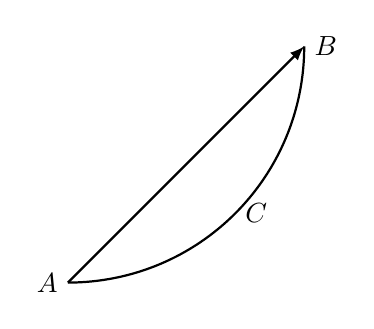
\begin{tikzpicture}[>=latex, thick]
  \draw [->](0,0)node[left]{$A$} --(3,3)node [right]{$B$} ;
  \draw (0,0) [bend left=-45]  to node [right]{$C$} (3,3);
\end{tikzpicture}
\end{document}
\chapter{电场}\label{chp:electric_field}
人类很早就认识了磁现象和电现象。
例如,我国在战国末期就发现了磁铁矿吸引铁的现象,在东汉初年就有带电的琥珀吸引轻小物体的文字记载。
但是,人类对电磁现象的系统研究却是在欧洲文艺复兴之后逐渐开展起来的,到十九世纪才建立了完整的电磁学理论。
电磁学及其应用对人类的影响十分巨大。
电力工业和电子技术是四个现代化建设的重要部门,电磁学理论是人们探索客观世界的有力武器。
所以我们应当学好电磁学。

\section{两种电荷\texorpdfstring{\quad}{ }电荷守恒定律}
\subsection{两种电荷} 
在初中已经学过,用毛皮摩擦过的硬橡胶棒,或用丝绸摩擦过的玻璃棒都能吸引轻小物体,即它们都带上了电荷。
玻璃棒上带的电荷叫正电荷,硬橡胶棒上带的电荷叫负电荷。
自然界只存在两种电荷,而且同种电荷互相排斥,异种电荷互相吸引。
电荷是有多有少的,电荷的多少叫做电量。

如\cref{fig:6-1a} 所示,让验电器带上适量正电荷,这时验电器的金属箔张开。
如果用带正电的玻璃棒接触验电器的金属球,把正电荷传给验电器,金属箔张开的角度就变大(\cref{fig:6-1b});如果用带负电的硬橡胶棒接触验电器的金属球,把负电荷传给验电器,金属箔张开的角度就变小(\cref{fig:6-1c})。
可见,同种电荷放在一起互相增强,异种电荷放在一起互相减弱或抵消。
通常,正电荷的电量用正数来表示,负电荷的电量用负数来表示。

\begin{figure}
	\begin{minipage}{0.3\linewidth}\centering
		\includegraphics{6-1a.pdf}
		\subcaption{}\label{fig:6-1a}
	\end{minipage}
	\begin{minipage}{0.3\linewidth}\centering
		\includegraphics{6-1b.pdf}
		\subcaption{}\label{fig:6-1b}
	\end{minipage}
	\begin{minipage}{0.3\linewidth}\centering
		\includegraphics{6-1c.pdf}
		\subcaption{}\label{fig:6-1c}
	\end{minipage}
	\caption{}\label{fig:6-1}
\end{figure}

等量的异种电荷完全相互抵消的现象叫做中和。
我们知道,物体是由原子组成的,原子是由带正电的原子核和带负电的电子组成的。
在通常的情况下,原子核所带的正电荷的电量(绝对值)等子所有电子所带负电荷的电量的总和(绝对值),原子呈中性状态,物体也呈中性状态,即对外表现为不带电的状态。
任何不带电的物体,其中都有等量的正负电荷,因而处于中性状态。

使物体带电叫做起电。
起电的过程,实际上是使物体中的正负电荷分开的过程。
在摩擦起电中,其中一个物体因失去一些电子而带正电,同时另一个物体因得到这些电子面带等量的负电。
摩擦起电并不是创造了电荷,只是电荷从一个物体转移到另一个物体。

\subsection{静电感应} 

还有一种常见的使物体带电的方法叫感应起电。
取一对用绝缘柱支持的金属导体 $A$ 和$B$,导体上都贴有金属箔,让 $A$ 和 $B$ 彼此接触,这时 $A$ 和 $B$ 上的金属箔闭合,表示它们都没有带电。
把另一个带正电的金属球 $C$ 移近导体 $A$(\cref{fig:6-2a}),这时
\begin{figure}
	\begin{minipage}[b]{0.45\linewidth}\centering
		\includegraphics{6-2a.pdf}
		\subcaption{}\label{fig:6-2a}
	\end{minipage}
	\begin{minipage}[b]{0.45\linewidth}\centering
		\includegraphics{6-2b.pdf}
		\subcaption{}\label{fig:6-2b}
	\end{minipage}
	\caption{静电感应}\label{fig:6-2}
\end{figure}
$A$、$B$ 上的金属箔都张开了,表示它们都带了电。
实验表明,靠近 $C$ 的导体 $A$ 带的电荷与 $C$ 异号,远离 $C$ 的导体 $B$ 带的电荷与 $C$ 同号。
这种现象叫做\Concept{静电感应}。
如果先把 $A$ 和 $B$ 分开,然后移去 $C$,则发现 $A$ 和 $B$ 仍带有电荷(\cref{fig:6-2b})。
如果再让 $A$ 和 $B$ 重新接触,它们就呈现不带电的状态。
这说明:$A$ 和 $B$ 分开后所带的异种电荷是等量的,重新接触后等量异种电荷相互抵消。
利用静电感应使物体带电的方法叫做\Concept{感应起电}。

\subsection{电荷守恒定律} 
静电感应也是使物体中的电荷分开,当我们把带正电的导体 $C$ 移近绝缘导体时(\cref{fig:6-2b}),绝缘导体里的自由电子被吸引过来,因此导体两端分别带上等量异种电荷。
可见,静电感应也不是创造了电荷,只是电荷从物体的一部分转移到另一部分。

大量事实说明:\emph{电荷既不能创造,也不能被消灭,它们只能从一个物体转移到另一个物体,或者从物体的一部分转移到另一部分}。
这个结论叫做\Concept{电荷守恒定律}。
它是物理学中重要的基本定律之一。

\begin{Practice}
\begin{question}
\item 把支在绝缘座上的不带电的导体 $A$ 移近带电体 $B$,用手指接触一下 $A$,然后移开手指,握住绝塚座移开导体 $A$,导体 $A$ 就带电了。如果带电体 $B$ 原来带正电,导体 $A$ 将带什么电?做这个实验并作出解释,实验时可用验电器来检查导体 $A$ 是否带电和带什么电。
\item 在\cref{fig:6-1}中,先让验电器带上少量正电荷,然后拿一个带负电的带电体逐渐接近验电器的金属球,可以看到这样的现象:金属箔张开的角度先是减小,以至闭合,然后又张开了。解释这个现象。
\end{question}
\end{Practice}

\section{库仑定律}
\subsection{库仑定律} 
两个电荷间的相互作用力,跟它们的电量有关系,还跟电荷间的距离有关系。
法国物理学家库仑(1736--1806)用实验研究了静止的点电荷间的相互作用力,于 1785 年发现了后来用他的名字命名的定律。

什么是点电荷呢?如果带电体间的距离比它们的大小大得多,以致带电体的形状和大小对相互作用力的影响可以忽略不计,这样的带电体就可以看成是点电荷。
跟力学中质点的概念类似,点电荷这个概念也是一种科学的抽象,是一种理想化的模型。

\medskip\noindent
\begin{minipage}{0.55\linewidth}\parindent2em
库仑是用\cref{fig:6-3} 所示的扭秤来做实验的。
扭秤的主要部分是在一根细金属丝下面悬挂一根玻璃棒,棒的一端有一个金属小球 $A$,另一端有一个平衡小球 $B$。
在离 $A$ 球某一距离的地方再放一个同样的金属小球 $C$。
如果 $A$ 球和 $C$ 球带同种电荷,它们间的斥力将使玻璃棒转过一个角度。
向相反方向扭转旋钮 $M$,使玻璃棒回到原来的位置并保持静止,这时金属丝扭转弹力的力矩跟电荷间斥力的力矩平衡。
因此从旋钮 $M$ 转过的角度可以计算出电荷间作用力的大小。
\end{minipage}\hfill
\begin{minipage}{0.4\linewidth}\centering
	\begin{figurehere}
		\includegraphics{6-3.pdf}
		\caption{库仑扭秤}\label{fig:6-3}
	\end{figurehere}
\end{minipage}

\medskip
库仑的实验是要研究电荷间的相互作用力跟它们间的距离和电量的关系。
作用力跟距离的关系比较好办,保持两球的电量不变,改变两球的距离并测出作用力,就可以找出作用力跟距离的关系。
困难在于作用力跟电量的关系,因为当时还不知道怎样测量电量,甚至连电量的单位也没有确定。
库仑找到了一个简单办法巧妙地解决了这个问题。
他把一个带电的金属球跟同样的但不带电的金属球相碰,两球带的电量一定相等,都是原有电量的 1/2。
同样可以得到原有电量的 1/4、1/8 等等的电量。
这样就可以用扭秤来研究电荷间的作用力跟电量的关系了。
库仑实验是在空气中做的,其结果跟在真空中相差很小。
库仑实验的结果是:\emph{在真空中两个点电荷间的作用力跟它们的电量的乘积成正比,跟它们间的距离的平方成反比,作用力的方向在它们的连线上}。
这就是\Concept{库仑定律}。
电荷间的这种作用力叫做\Concept{静电力},又叫做\Concept{库仑力}。

如果用 $Q_1$、$Q_2$ 表示两个点电荷的电量,用 $r$ 表示它们间的距离,用 $F$ 表示它们间的静电力,库仑定律就可以写成下面的公式:
\begin{equation}
F=k\frac{Q_1Q_2}{r^2}.
\end{equation}
式中 $k$ 是比例恒量,叫\Concept{静电力恒量},它的数值和单位由式中各量的单位决定。

我们很容易看出,库仓定律和万有引力定律很相似,它们都是平方反比定律。
人们现在还不能说明为什么这两个定律如此相似,但这种相似使我们可以用力学的比喻来理解许多电学问题,给我们的学习带来不少方便。

\subsection{电介质中的库仑定律} 
所谓电介质,就是我们在初中学过的绝缘体。
空气、煤油、水、玻璃、橡胶、瓷器等都是电介质。

如果把两个电荷放在电介质里,例如放在煤油里,电荷间的作用力就比在同样情形下在真空里的作用力小。小多少,依电介质的不同而不同。这时库仑定律用下面公式来表示:
\begin{equation}
F=k\frac{Q_1Q_2}{\varepsilon r^2}.
\end{equation}

每一种电介质的 $\varepsilon$ 的数值是一定的,叫做那种物质的\Concept{介电常数},\cref{tab:6-1} 是几种电介质的介电常数。
实用上,通常把空气的介电常数取为 1,即认为电荷间的作用力在空气中跟在真空中一样。

\begin{table}
	\caption{几种电介质的介电常数}\label{tab:6-1}
	\begin{tblr}{colspec={c*{7}{X[r]}},hline{2}=0.8pt,vline{2}=0.8pt,row{1}={m,c}}
 电介质  & 空气   &煤油 &石蜡 &陶瓷 & 玻璃 & 云母 & 水\\
介电常数 & \num{1.0005} &2 &\numrange{2.0}{2.1}& 6 &\numrange{4}{11}&\numrange{6}{8}&81\\
	\end{tblr}
\end{table}

\subsection{电量的单位} 
在国际单位制中,电量的单位就是我们在初中学过的\Concept{库仑},简称\Concept{库},国际符号是 \unit{C}。

采用国际单位制,在库仑定律的公式中,力的单位用牛,距离的单位用米,电量的单位用库,各个量的单位都已经分别确定,这时静电力恒量的数值要由实验来确定,实验指出:公式中的静电力恒量 $k=\qty{9.0e9}{N.m^2/C^2}$。

\begin{example}
比较电子和质子间的静电引力和万有引力,已知电子质量是 \qty{0.91e-30}{kg},质子质量是 \qty{1.67e-27}{kg},电子和质子的电量都是 \qty{1.60e-19}{C}。
\end{example}
	
\begin{solution}
电子和子间的静电引力 $F_{\text{电}}$ 和万有引力 $F_{\text{引}}$ 分别是
\[F_{\text{电}} =k\frac{Q_1Q_2}{r^2} ,\qquad   F_{\text{引}}=G\frac{m_1m_2}{r^2}, \]
因此,
\[\frac{F_{\text{电}}}{F_{\text{引}}}=\frac{kQ_1Q_2}{Gm_1m_2}.\]

上式中 $m_1$、$m_2$ 和 $Q_1$、$Q_2$ 已知,$k=\qty{9.0e9}{N.m^2/C^2}$,$G=\qty{6.67e-11}{N.m^2/kg^2}$。把数值代入进行计算,得
\[\begin{split}
	\frac{F_\text{电}}{F_\text{引}}&=\frac{\num{9.0e9}\times\num{1.60e-19}\times\num{1.60e-19}}{\num{6.67e-11}\times \num{1.67e-27}\times \num{0.91e-30}}.\\
	&=\num{2.3e39}
\end{split}\]
\end{solution}

从这个例题可以看出,电子和质子间的万有引力比它们的静电引力小得多。
正是因为这个缘故,在研究微观带电粒子间的(如原子中电子和原子核间的)相互作用时,经常把万有引力忽略不计。

\begin{Practice}
\begin{question}
	\item \qty{1}{C} 的电量是电子所带电量的多少倍?
	\item 在真空中有两个点电荷,电量分别为 \qty{+4.0e-9}{C} 和 \qty{+2.0e-9}{C} ,相距 \qty{10}{cm},这两个点电荷间的作用力是多大?用电荷的绝对值代入进行计算,求出力的大小,然后根据电荷的正负确定是引力还是斥力。
	\item 在真空中有两个点电荷,保持它们的距离不变,它们间的相互作用力在下列情况下将如何变化?
	\begin{tasks}
		\task 一个电荷的电量变为原来的 2 倍;
		\task 两个电荷的电量都变为原来的 1/2。
	\end{tasks}
	\item 原子核的半径大约为 \qty{e-14}{m},假定核中两个质子相距这么远,其间的静电力大约有多大?
	\item 两个带电小球在煤油中相距 \qty{0.5}{m},其中一个小球带电 \qty{5.0e-9}{C},另一个带电 \qty{3.0e-9}{C},求小球间的作用力。
	\item 当两个点电荷相距为 $r$ 时,它们间的斥力为 $F$。改变电荷间的距离,当斥力为 $16F$ 时,相距为多少?当斥力为 $\dfrac{1}{4}F$ 时,相距为多少?
\end{question}
\end{Practice}

\section{电场\texorpdfstring{\quad}{ }电场强度}

\subsection{电场}
电荷间的相互作用是怎样发生的呢?

经过长期的科学研究,人们认识到:电荷之间的相互作用是通过电场发生的。
只要有电荷存在,电荷周围就存在着电场;电场的基本性质是它对放入其中的电荷有力的作用,这种力叫做电场力。
两个电荷 $A$ 和 $B$,电荷 $A$ 受到的电荷 $B$ 的作用,实际上是电荷 $B$ 的电场对电荷 $A$ 的作用。
同样,电荷 $B$ 受到的电荷 $A$ 的作用,实际上是电荷 $A$ 的电场对电荷 $B$ 的作用。

历史上人们对场的认识是逐步深入的,我们理解场这个概念也要有个过程,要逐步体会它的意义。
引入场这个概念,是对物理学的重要贡献。
场的概念引入物理学之后取得了巨大的成果。
除了电场,我们在初中还学过磁场,电场和磁场是有联系的,常常总称为电磁场。
关于电磁场的研究导致了发现电磁波。
我们大家都熟悉的广播和电视就是借电磁波来传播的。
电磁波可以脱离电荷而独立存在并以光速传播,它跟由原子、分子组成的物质一样具有能量和动量。
这样,人们逐渐认识到:电磁场包括电场和磁场是物质的一种特殊形态。

电场这种物质跟由分子、原子组成的物质不同,看不见,摸不到,好象不好理解。
其实,电场跟其他物质一样,都是不依赖于我们的感觉而客观存在的东西。
在一位现代物理学家看来,电场正象他所坐的椅子一样是客观存在。
电场是在跟电荷的相互作用中表现出自己的特性的。
我们从电场所表现出来的特性出发,加以分析研究,就可以懂得电场,认识电场。

\subsection{电场强度} 

刚刚说过,电场的基本性质是它对放入其中的电荷有电场力的作用,现在来分析研究这个问题。

要研究电场,必须在电场中放入电荷,而这个电荷应该是一个电量很小的点电荷。
电量很小,是为了使它放入之后,不致影响原来要研究的电场。
体积很小,是为了便于用它来研究电场各点的性质。
这样的电荷常常叫做检验电荷。
\begin{figure}
	\begin{minipage}[b]{0.4\linewidth}\centering
		\includegraphics{6-4a.pdf}
		\subcaption{}\label{fig:6-4a}
	\end{minipage}
	\begin{minipage}[b]{0.56\linewidth}\centering
		\includegraphics{6-4b.pdf}
		\subcaption{}\label{fig:6-4b}
	\end{minipage}
	\caption{}\label{fig:6-4}
\end{figure}

如\cref{fig:6-4} 所示,电场是由正电荷 $Q$ 产生的,用挂在丝线下端的带正电的小球作检验电荷,把它先后放在电场中不同的位置,观察它在电场中的受力情况,力的大小可以从丝线对竖直线偏角的大小看出。
实验表明,检验电荷在电场中的位置不同,受到的电场力的大小和方向也不同。
检验电荷受到的电场力大,说明那点的电场强;检验电荷受到的电场力小,说明那点的电场弱。
\cref{fig:6-4b} 中 $A$ 点的电场强,$B$ 点的电场弱,$C$ 点更弱。

物理学中怎样来表示电场的强弱呢?
把检验正电荷 $q$ 放到电场中的 $A$ 点,电荷 $q$ 受到电场力 $F_A$ 的作用(\cref{fig:6-4b})。
设 $A$ 点跟 $Q$ 的距离为 $r_1$,从库仑定律知道 $F_A=kQq/r^2_1$。
同样,如果把正电荷 $q'$ 放入 $A$ 点,$q'$ 受到的电场力 $F'_A=kQq'/r_1^2$。
可以看出,
\[\frac{F_A}{q}=\frac{F'_A}{q'}=\frac{kQ}{r^2_1}.\]
这就是说,放入 $A$ 点的电荷受到的电场力跟它的电量的比值,是一个跟放入该点的电荷无关的恒量。

如果把电荷放入电场中的 $B$ 点和 $C$ 点,设 $B$、$C$ 跟 $Q$ 的距离分别为 $r_2$ 和$r_3$,同样可以证明,电荷在 $B$ 和 $C$ 受到的电场力跟它的电量的比值分别是 $kQ/r^2_2$、$kQ/r_3^2$,都是跟放入的电荷无关的恒量。

可见,电荷在电场中某一点受到的电场力跟它的电量的比值,由该点在电场中的位置所决定,跟放入的电荷无关。
这个比值越大的地方,放入那里的单位电荷受到的电场力越大,电场就越强。
这一点不仅对正电荷 $Q$ 产生的电场是适用的,对任何电场都是适用的。
这就是说,对任何电场,都要用上述比值来表示电场的强弱。

放入电场中某一点的电荷受到的电场力跟它的电量的比值,叫做这一点的\Concept{电场强度},简称为\Concept{场强}。
跟力一样,电场强度也是矢量,如果用 $E$ 表示电场强度,用 $F$ 表示检验电荷 $q$ 受到的电场力,那么
\begin{equation}
	\label{eq:electric_field_strength}
	E=\frac{F}{q}.
\end{equation}

由\cref{eq:electric_field_strength} 可以知道,如果 $q$ 为单位正电荷,那么 $E$ 和 $F$ 在数值上相等,可见电场中某一点的场强在数值上等于单位正电荷在那一点所受的电场力。
正负电荷在电场中某点所受电场力的方向相反。
我们规定场强的方向是正电荷受力的方向。
这样,负电荷受力的方向跟场强的方向相反。

场强的单位是牛/库(\unit{N/C})。电场中的某一点,如果 \qty{1}{C} 的点电荷在该点受到的电场力是 \qty{1}{N},这点的场强就是 \qty{1}{N/C}。

从上面讲的很容易知道,点电荷 $Q$ 在真空中形成的电场中,在距离 $Q$ 为 $r$ 的 $P$ 点的场强 $E$ 的大小为 
\begin{equation}
	\label{eq:electric_field_strength_point}
	E=\frac{kQ}{r^2}.
\end{equation}

这个公式只适用于真空,如果在充满电介质的空间里,这个公式应改写成
\begin{equation}
	\label{eq:electric_field_strength_point_media}
	E=\frac{kQ}{\varepsilon r^2}.
\end{equation}

如果 $Q$ 是正电荷,$E$ 的方向就背离 $Q$;如果 $Q$ 是负电荷,$E$ 的方向就指向 $Q$(\cref{fig:6-5})。
\begin{figure}
	\includegraphics{6-5.pdf}
	\caption{场强的方向}\label{fig:6-5}
\end{figure}

应该注意,\cref{eq:electric_field_strength,eq:electric_field_strength_point,eq:electric_field_strength_point_media} 虽然都表示电场中某点的场强,但它们的意义是不同的。
\cref{eq:electric_field_strength} 是场强的定义式,对任何电场都适用。
\cref{eq:electric_field_strength_point} 是点电荷在真空中各点场强的计算式,只适用于点电荷在真空中的电场。
\cref{eq:electric_field_strength_point_media} 是点电荷在充满电介质空间里各点场强的计算式。

如果有几个点电荷同时存在,它们的电场就互相叠加,形成合电场,这时某点的场强,就等于各个点电荷在该点产生的场强的矢量和。
这样,知道了点电荷的场强,原则上我们就可以知道任一带电体的场强,因为任何带电体都可以看作是由许多点电荷组成的。

\begin{Reading}{用比值定义物理量}
在物理学中,常常用比值来定义一个物理量。

我们在初中学过密度,在那里我们学到:单位体积的某种物质的质量,叫做这种物质的密度。
其实,密度也可以用比值来定义。
某种物质的物体,它的质量与它的体积成正比。
因此我们可以这样表达密度的定义:某种物质组成的物体,它的质量和它的体积的比值,叫做这种物质的密度。
对某种物质来说,这个比值是恒定的;对不同的物质来说,这个比值一般并不相同。
因此,密度表示物质的一种特性。

初中学过的电阻是用比值来定义的。
一段导体中的电流强度跟加在这段导体上的电压成正比,导体两端的电压跟通过导体的电流强度的比值,叫做这段导体的电阻。
当温度保持不变时,对某段导体来说,这个比值是恒定的;对不同的导体来说,这个比值一般并不相同。
这个比值越大,表示导体对电流的阻碍作用越大。
因此,电阻是表示导体对电流阻碍作用的物理量。

刚刚学过的电场强度也是用比值来定义的。
放入电场中某点的电荷受到的电场力跟它的电量成正比。
放入电场中某点的电荷受到的电场力跟它的电量的比值,叫做这一点的电场强度。
对电场中的某一点,这个比值是恒定的;对电场中的不同的点,这个比值一般并不相同。
这个比值越大,表示那一点的电场越强。电场强度是表示电场的力的性质的物理量。

不再一一列举。我们看到这里有一个共同点,那就是要在实验的基础上寻求一个只与所研究的物体或场有关的比值,来表示物体或场的某种性质,并由这个比值定义一个新的物理量。
在定义这个新的物理量的同时,也就确定了这个新的物理量与已有物理量之间的关系。
例如,定义了密度,也就确定了密度、体积和质量这三者的关系。
这里我们一定要注意到这个比值是反映物体或场的什么性质,这样才能很好地理解它的物理意义。

在今后的学习中,还会遇到用比值来定义的物理量。因此,我们要很好地体会这种定义物理量的方法。
\end{Reading}

\begin{Practice}
\begin{question}
	\item 在正电荷 $Q$ 的电场中的某一点放一个电荷,它的电量 $q=\qty{e-8}{C}$,$q$ 受到的电场力为 \qty{e-8}{N}。求这一点的电场强度 $E$,并指出电场强度的方向。如果取走 $q$,$E$ 有无变化?为什么?
	\item 在以水为介质的负点电荷 $Q$ 的电场中,离 $Q$ \qty{0.5}{m} 处的电场强度 $E$ 是 \qty{1}{N/C},求负电荷 $Q$ 的电量是多少库。
	\item 电场中某点的场强是 \qty{0.2e5}{N/C}。求电量为 \qty{2e-8}{C} 的正电荷在该点受到的电场力是多大。
	\item 在氢原子中,电子和质子的平均距离是 \qty{5.3e-11}{m}。质子在这个距离处产生的场强是多大?方向如何?电子受到的力是多大?方向如何?
	\item 物理学上常把重力作用的空间叫做\Concept{重力场}。如果把单位质量的物体受到的重力叫做重力场强度,试写出重力场强度的定义式。重力场强度的方向如何?从重力场强度的方向来看,重力场是跟正电荷形成的电场相似,还是跟负电荷形成的电场相似?
	\item 电场强度的定义式 $E=F/q$ 在电介质中要不要改写?为什么?
\end{question}
\end{Practice}

\section{电力线}
\subsection{电力线}

研究电场,重要的是要知道电场中各点场强的大小和方向。
如果能够用图形把电场中各点场强的大小和方向形象地表示出来,这对我们认识电场是很有好处的。
\cref{fig:6-6} 是在正电荷和负电荷的电场中画出的一组矢量,表示出场内一些点的场强的大小和方向。
但是,更好的办法是用英国物理学家法拉第(1791--1867)引入的电力线来形象地表示电场。
\begin{figure}
	\includegraphics{6-6.pdf}
	\caption{}\label{fig:6-6}
\end{figure}

在任何电场中,每一点的场强 $B$ 都有一定的方向,所以我们可以在电场中画出一系列的从正电荷出发到负电荷终止的曲线,使曲线上每一点的切线方向都跟该点的场强方向一致,这些曲线就叫做\Concept{电力线}。
\cref{fig:6-7} 是一条电力线,它上面的 $A$、$B$ 点的场强 $E_A$、$E_B$ 在各该点的切线上,方向如图中箭头所示。
\begin{figure}
	\includegraphics{6-7.pdf}
	\caption{}\label{fig:6-7}
\end{figure}

电力线的形状可以用实验来观察。把奎宁的针状结晶、木屑或头发屑悬浮在蓖麻油里,再放入电场中,就可以看到微屑按照场强的方向排列起来(\cref{fig:6-8}),显示出电力线的形状。
应该注意,虽然我们可以用实验来显示电力线的形状,但电力线并不是电场里实际存在的线,而是人们为了使电场形象化而假想的线。
\begin{figure}
	\begin{minipage}{0.48\linewidth}\centering
		\includegraphics[height=3.8cm]{6-8a.jpg}
		\subcaption{点电荷的电力线形状}\label{fig:6-8a}
	\end{minipage}
	\begin{minipage}{0.48\linewidth}\centering
		\includegraphics[height=3.8cm]{6-8b.jpg}
		\subcaption{带相反电荷的平行板间的电力线形状}\label{fig:6-8b}
	\end{minipage}
	\caption{}\label{fig:6-8}
\end{figure}

\cref{fig:6-9} 是点电荷的电力线,\cref{fig:6-10} 是两个等量的电荷的电力线。
从图中可以看出,在离形成电场的电荷越近的地方,也就是场强越大的地方,电力线越密。所以,用电力线不但可以形象地表示电场强度的方向,还可以表示电场强度的大小:场强越大的地方电力线越密,场强越小的地方电力线越稀。

\begin{figure}
	\begin{minipage}[b]{0.48\linewidth}\centering
		\includegraphics{6-9a.pdf}
		\subcaption{正电荷}\label{fig:6-9a}
	\end{minipage}
	\begin{minipage}[b]{0.48\linewidth}\centering
		\includegraphics{6-9b.pdf}
		\subcaption{负电荷}\label{fig:6-9b}
	\end{minipage}
	\caption{点电荷的电力线}\label{fig:6-9}
	\begin{minipage}[b]{0.48\linewidth}\centering
		\includegraphics{6-10a.pdf}
		\subcaption{等量异种电荷}\label{fig:6-10a}
	\end{minipage}
	\begin{minipage}[b]{0.48\linewidth}\centering
		\includegraphics{6-10b.pdf}
		\subcaption{等量同种电荷}\label{fig:6-10b}
	\end{minipage}
	\caption{两个等量电荷的电力线}\label{fig:6-10}
\end{figure}

\subsection{匀强电场} 

在电场的某一区域里,如果各点的场强的大小和方向都相同,这个区域的电场就叫做\Concept{匀强电场}。
匀强电场是最简单的同时也是很重要的电场,在实验研究中常常要用到它。

在匀强电场里,既然各点的场强的方向都相同,电力线就一定是互相平行的直线;既然各点的场强的大小都相同,电力线的疏密程度也一定处处相等。
因此,匀强电场中的电力线是距离相等的互相平行的直线。

两块靠近的平行金属板,它们的大小相等并且互相正对,在分别带等量的正电和负
电的时候,它们之间的电场,除边缘附近外,就是匀强电场(\cref{fig:6-11})。

\begin{figure}
	\includegraphics[angle=90]{6-11.pdf}
	\caption{匀强电场}\label{fig:6-11}
\end{figure}

\begin{Reading}{法拉第和场的概念}
相隔一定距离的电荷或磁体间的相互作用是怎样发生的,这个问题在历史上有过长期的争论。
十九世纪前期,大部分物理学家认为电荷或磁体间的相互作用是超距作用。
所谓超距作用是指这种作用不需要任何媒质传递,就能够由一个物体立即作用到另一个物体。

然而法拉第通过实验发现,电作用或磁作用跟电荷之间或磁体之间的媒质有关。
他在不同的媒质中进行同样的实验,其作用效果不同。
这引起他对电磁作用本质的深思。
法拉第认为,电磁力不可能是超越空间并与空间中媒质无关的超距作用。
法拉第提出了关于电磁作用的新看法:电荷或磁体在周围空间产生电场或磁场,正是通过场,才把电作用或磁作用传递到别的电荷或磁体。

经典力学是以超距作用为基础的,空间中除了粒子以外什么也没有,没有粒子的地方是一无所有的真空;粒子间的相互作用是超距作用,不需要通过媒质传递。
法拉第提出的场的模型从基本概念上突破了经典力学的框架,为建立近代物理开创了新的起点。

法拉第凭着敏锐的直觉不仅提出了场的概念,而且描绘出一幅清晰的场的图象。
他用电力线或磁力线形象地表示电场和磁场。
力线密的地方场就强,力线疏的地方场就弱。
力线上每一点的切线方向表示场强的方向。
法拉第用这幅图象解释了用经典力学无法解释的现象。
例如,1831 年他发现了电磁感应现象,他借助于磁力线对这一现象很快地作出了解释:只要通过闭合电路的磁力线数目发生变化,电路里就会产生电流。

法拉第提出的场的概念还处于萌芽状态。
后来麦克斯韦用数学方程定量地描述了电磁场的定律,预言了电磁波的存在,并且把光现象和电磁现象联系起来,得出光波是一种电磁波的结论。
场的概念取得了很大成功,并逐渐在物理学中取得了主要地位,是基本的物理概念之一。
\end{Reading}

\begin{Practice}
\begin{question}
	\item 有人说电力线就是带电粒子在电场中运动的轨迹。这种说法对吗?为什么?
	\item 在\cref{fig:6-9,fig:6-10,fig:6-11} 中,所有的电力线都不相交,我们能否断言,电场中任何两条电力线都不相交,为什么?
\end{question}
\end{Practice}

\section{电场中的导体}
我们在初中学过,导体的特征是它的内部有大量的可以移动的自由电荷。
对于金属导体来说,这种自由电荷就是自由电子。
金属原子的最外层电子跟原子核的联系很弱,在其余原子的作用下会脱离原来的原子而在整块金属中自由“游荡”,成为自由电子。
失去了外层电子的原子变成带正电的离子,在平衡位置附近做热振动。
所以,整块金属就是由做热振动的正离子和在它们之间做无规则的热运动的自由电子组成的。

\subsection{静电平衡状态} 
\begin{figure}
	\begin{minipage}[b]{0.33\linewidth}\centering
	  \includegraphics{6-12a.pdf}
		\subcaption{}\label{fig:6-12a}
	\end{minipage}
	\begin{minipage}[b]{0.33\linewidth}\centering
	  \includegraphics{6-12b.pdf}
		\subcaption{}\label{fig:6-12b}
	\end{minipage}
	\begin{minipage}[b]{0.3\linewidth}\centering
	  \includegraphics{6-12c.pdf}
		\subcaption{}\label{fig:6-12c}
	\end{minipage}
	\caption{}\label{fig:6-12}
\end{figure}

把一个不带电的金属导体 $ABCD$ 放到场强为 $E_0$ 的电场中,导体内部的自由电子受到电场力的作用,将向电场的反方向做定向移动(\cref{fig:6-12a})。
这样,在金属的 $AB$ 面上将出现负电荷,在 $CD$ 面上将出现正电荷。
这种导体里的自由电荷由于受到外电场的作用而重新分布的现象,就是我们前面讲过的静电感应。
导体两端出现的正负电荷在导体内部形成反方向的电场 $E'$,它的电力线用虚线表示(\cref{fig:6-12b})。
这个电场与外电场叠加,使导体内部的场强减小。
但是,只要导体内部的场强不等于零,自由电子就继续移动,两端的正负电荷就继续增加,导体内部的电场就进一步削弱,直到导体内部各点的场强都等于零时为止。
这时自由电子的定向移动停止(\cref{fig:6-12c})。

导体中(包括表面)没有电荷定向移动的状态叫做\Concept{静电平衡状态}。
\emph{处于静电平衡状态的导体,内部的场强处处为零}。

导体处静电平衡状态时,它表面的场强方向一定与其表面垂直(参看\cref{fig:6-12c})。
假如不是这样,场强就有一个沿导体表面的分量,导体上的自由电子就会发生定向移动,这就不是平衡状态了。
所以,\emph{处于静电平衡状态的导体,表面上任何一点的场强方向跟该点的表面垂直}。

带电导体可以认为它处于本身所带电荷形成的电场中,它在静电平衡状态时内部的场强也一定处处为零。
假如不是这样,导体内部的自由电子就会发生定向移动。
既然导体内部的场强处处为零,导体内部就不可能有未被抵消的电荷。
这是因为,假如在导体内部某处有电荷,在它的附近的场强就不可能为零。
所以,\emph{处于静电平衡状态的带电导体,电荷只能分布在导体的外表面上}。

静电平衡时电荷只分布在导体的外表面上,可以用下述的法拉第圆筒实验来验证。
如\cref{fig:6-13} 所示,取两个验电器 $A$ 和 $B$,在 $B$ 上装一个几乎封闭的空心金属圆筒 $C$(叫做法拉第圆筒)。
使 $B$ 和 $C$ 带电,$B$ 的箔片张开,用有绝缘柄的金属小球 $e$ 先跟 $C$ 的外部接触,再把 $e$ 移到 $A$ 并跟 $A$ 的金属球接触(\cref{fig:6-13})。
经过若干次以后,可以看到 $A$ 的箔片张开,同时$B$ 的箔片张开的角度减小。这表明 $e$ 把 $C$ 的一部分电荷搬运给了 $A$。
可见法拉第圆筒的外表面是带有电荷的。
如果让 $e$ 不接触 $C$ 的外部,而接触 $C$ 的内部,重做上述实验(\cref{fig:6-14}),不论重复多少次,$A$ 的箔片都不张开,$B$ 的箔片张开的角度也
不减小。
这表明 $e$ 并没有把 $C$ 的电荷搬运给 $A$,可见拉法第圆筒的内部不带电。

\begin{figure}
	\begin{minipage}[b]{0.48\linewidth}\centering
		\includegraphics{6-13.pdf}
		\caption{}\label{fig:6-13}
	\end{minipage}
	\begin{minipage}[b]{0.48\linewidth}\centering
		\includegraphics{6-14.pdf}
		\caption{}\label{fig:6-14}
	\end{minipage}
\end{figure}

\subsection{静电屏蔽}
静电平衡时导体内部的场强为零这一现象,在技术上用来实现静电屏蔽。

如\cref{fig:6-15a} 所示,使带正电的金属球靠近验电器,由于静电感应,验电器的箔片张开,这表示验电器受到了附近的带电体的影响。
如果事先用一个金属网罩把验电器罩住(\cref{fig:6-15b}),
\begin{figure}
	\begin{minipage}[b]{0.48\linewidth}\centering
		\includegraphics{6-15a.pdf}
		\subcaption{}\label{fig:6-15a}
	\end{minipage}
	\begin{minipage}[b]{0.48\linewidth}\centering
		\includegraphics{6-15b.pdf}
		\subcaption{}\label{fig:6-15b}
	\end{minipage}
	\caption{静电屏蔽}\label{fig:6-15}
\end{figure}
再让带电金属球靠近,验电器的箔片就不张开了。
即使用导线把验电器和金属网罩连接上,箔片也不张开。
可见,金属网罩(或金属包皮)能把外电场遮住,使内部不受外电场的影响,这就是\Concept{静电屏蔽}。
有的电学仪器和电子设备的外面套有金属罩,通讯电缆的外面包一层铅皮,都是用来防止外界电场的干扰起屏蔽作用。

\section{电势能}
前面我们从电荷在电场中受到力的作用出发,研究了电场的性质。
下面我们从能量的角度来研究电场的性质。

我们知道,物体在重力场中具有重力势能。
重力势能是与重力做功密切相关的。
同样,电荷在电场中也具有势能,叫做电势能。
电势能是与电场力做功密切相关的。

物体在地面附近下落时,重力对物体做正功,重力势能减少;物体上升时,重力对物体做负功,重力势能增加。
重力势能的变化总等于重力对物体所做的功。
与此相似,在电场中移动电荷时,如果电场力对电荷做正功,电势能就减少;如果电场力对电荷做负功,电势能就增加。
电势能的变化总等于电场力对电荷所做的功。

就功和能之间的关系来讲,电场中的情形跟重力场中的情形完全相似。
但由于存在两种电荷,电场力既可以是引力,也可以是斥力,因此电场力做功的问题要复杂一些。

\cref{fig:6-16} 表示正电荷 $Q$ 的电场,在电场中把正电荷 $q$ 从 $A$ 点移到 $B$ 点,电场力的方向与电荷移动的方向相同,电场力对电荷 $q$ 做正功,电势能减少。
可见,正电荷 $q$ 在 $A$ 点的电势能大于它在 $B$ 点的电势能。
在正电荷 $Q$ 的电场中,正电荷 $q$ 离 $Q$ 越近,电势能越大。
\begin{figure}
	\begin{minipage}[b]{0.48\linewidth}\centering
		\includegraphics{6-16.pdf}
		\caption{正电荷 $Q$ 的电场}\label{fig:6-16}
	\end{minipage}
	\begin{minipage}[b]{0.48\linewidth}\centering
		\includegraphics{6-17.pdf}
		\caption{负电荷 $Q$ 的电场}\label{fig:6-17}
	\end{minipage}
\end{figure}

\cref{fig:6-17} 表示负电荷 $Q$ 的电场,在电场中把正电荷 $q$ 从 $C$ 点移到 $D$ 点,电场力的方向与电荷移动的方向相反,电场力对电荷 $q$ 做负功,电势能增加。
可见,正电荷 $q$ 在 $C$ 点的电势能小于它在 $D$ 点的电势能。
在负电荷 $Q$ 的电场中,正电荷 $q$ 离 $Q$ 越近,电势能越小。

我们在讨论重力势能的时候,要先规定物体在某一位置的重力势能为零,然后才能确定物体在其他位置的重力势能。
物体在某一位置的重力势能在数值上等于物体从这一位置移到重力势能为零处重力所做的功。
同样,我们在讨论电势能的时候,也要先规定电荷在某一位置的电势能为零,然后才能确定电荷在其他位置的电势能。
\emph{电荷在电场中某点的电势能在数值上等于把电荷从这点移到电势能为零处电场力所做的功}。

在理论研究中,通常取电荷 $q$ 在无限远处的电势能为零。
这样,在\cref{fig:6-16} 所示正电荷的电场中,因为正电荷 $q$ 在离开 $Q$ 越远的地方电势能越小,而它在无限远处的电势能为零,所以正电荷 $q$ 在正电荷 $Q$ 的电场中的电势能都是正值。
在\cref{fig:6-17} 所示的负电荷的电场中,因为正电荷 $q$ 在离开电荷 $Q$ 越远的地方电势能越大,而它在无限远处的电势能为零,所以正电荷 $q$ 在负电荷 $Q$ 的电场中电势能都是负值。

\begin{Practice}
\begin{question}
	\item 把两个异种电荷的距离增大一些,电场力做正功还是做负功?电势能是增加还是减小?把两个同种电荷的距离增大一些,情况又怎样?
	\item 在\cref{fig:6-16} 中,把负电荷 $-q$ 放在 $A$、$B$ 点,它在哪一点的电势能较大?无限远处的电势能为零,负电荷 $-q$ 在这个电场中的电势能是正值还是负值?
	\item 在\cref{fig:6-17} 中,把负电荷 $-q$ 放在 $C$、$D$ 点,它在哪一点的电势能较大?取无限远处的电势能为零,负电荷 $-q$ 在这个电场中的电势能是正值还是负值?
	\item 在\cref{fig:6-18} 所示的电场中,如果把正电荷 $q$ 由 $N$ 点移到 $M$ 点,$q$ 的电势能增加还是减小?如果移动的是负电荷 $-q$,电势能又怎样变化?
	\begin{figurehere}
    \begin{minipage}{\linewidth}\centering
			\includegraphics{6-18.pdf}
			\caption{}\label{fig:6-18}
		\end{minipage}
	\end{figurehere}	
	\item  电子在原子核附近运动时,电子的电势能是正值还是负值?取无限远处的电势能为零,把这个电子由原子核附近移到无限远处,电子的电势能是增加还是减小?
\end{question}
\end{Practice}


\section{电势}
电荷在电场中某点具有的电势能跟电荷所带的电量有关系。
设在\cref{fig:6-16} 所示的正电荷的电场中,正电荷 $q$ 在 $A$ 点的电势能为 $\mathcal{E}_A$,它在数上等于把电荷 $q$ 从 $A$ 点移到无限远处电场力所做的功。
如果把放在 $A$ 点的电荷增加为原来的 $n$ 倍,那么,在把它移到无限远处的过程中,所受的电场力处处为原来的 $n$ 倍,电场力所做的功也为原来的 $n$ 倍,因而电势能为原来的 $n$ 倍。
这就是说,电荷在电场中某点具有的电势能 $\mathcal{E}_A$ 跟电荷所带的电量 $q$ 成正比,不论电量 $q$ 是多少,比值 $\mathcal{E}_A/q$ 都相同,是跟电量 $q$ 无关的一个恒量。

把正电荷 $q$ 放在\cref{fig:6-16} 中的 $B$ 点,设电荷的电势能为 $\mathcal{E}_B$。
根据同样的分析知道,比值 $\mathcal{E}_B/q$ 也是跟电量无关的恒量。
因为 $\mathcal{E}_B$ 跟 $\mathcal{E}_A$ 一般并不相同,所以比值 $\mathcal{E}_B/q$ 跟 $\mathcal{E}_A/q$ 一般也不相同。

上面是就正电荷 $Q$ 产生的电场来分析的,实际上,上述分析对任何电场都是适用的。

既然在电场中某点比值 $\mathcal{E}/q$ 是跟电量 $q$ 无关的恒量,而且对电场中不同的点来说这个恒量一般并不相同,可见,这个恒量是由电场本身决定的,它反映电场本身的一种性质。

\emph{电场中某点的电荷的电势能跟它的电量的比值,叫做这一点的}\Concept{电势},如果用 $U$ 表示电势,用表示电荷 $q$ 的电势能,那么
\[U=\frac{\mathcal{E}}{q}.\]

如果取 $q$ 为单位正电荷,那么 $U$ 在数值上等于 $\mathcal{E}$。可见,电场中某点的电势在数值上等于单位正电荷在那一点所具有的电势能。

在国际单位制中,电势的单位是\Concept{伏特},简称伏,国际符号是 \unit{V}。电场中的某一点,如果电量是 \qty{1}{C} 的电荷在该点的电势能是 \qty{1}{J},这一点的电势就是 \qty{1}{V}。
\[ \qty{1}{V}=\qty{1}{J/C}.\]

电势只有大小,没有方向,因此是标量。

电势跟电势能一样,并没有绝对的意义。
只有先规定了某处的电势为零以后,才能确定电场中其他各点的电势的值。
电场中电势为零的位置也就是电荷在该点的电势能为零的位置。
在理论研究中,通常也就取无限远处的电势为零。
在实际应用中,通常取大地的电势为零。

在规定了零电势后,电场中各点的电势可以是正值,也可以是负值。
例如,规定无限远处的电势为零,在\cref{fig:6-16} 所示的正电荷 $Q$ 的电场中,因为正电荷 $q$ 的电势能都是正值,所以电场中各点的电势都是正值,而且离正电荷 $Q$ 越远,电势越低;在\cref{fig:6-17} 所示的负电荷 $Q$ 的电场中,因为正电荷 $q$ 的电势能都是负值,所以电场中各点的电势都是负值,而且离负电荷 $Q$ 越远,电势越高。

在电场中,我们可以根据电力线的方向判断电场中各点电势的高低。
因为顺着电力线的方向移动正电荷,电场力做正功,正电荷的电势能减小,所以\emph{顺着电力的方向电势越来越低}。
这个结果不但对正电荷或负电荷的电场是适用的,对任何电场都适用。

现在我们已经认识了反映电场性质的两个物理量:电场强度和电势。
\emph{电场强度是反映电场的力的性质的物理量}。
知道了电场强度 $E$,就可以知道电荷 $q$ 在电场中所受的力 $F=qE$。
\emph{电势是反映电场的能的性质的物理量}。
知道了电势 $U$,就可以知道电荷$q$ 在电场中的电势能 $\mathcal{E}-qU$。
在电势为正值的地方,正电荷的电势能是正值,负电荷的电势能是负值。
在电势为负值的地方,正电荷的电势能是负值,负电荷的电势能是正值。

\section{等势面}

我们知道,用电力线能够把电场中各点场强的大小和方向形象地表示出来。
电场中各点电势的大小,是否也可以用图形来表示呢?
同样可以,一般说来,电场中各点的电势不同,但电场中有许多点的电势相等。
我们把电场中电势相等的点构成的面叫做\Concept{等势面}。
在电场中可以用等势面来表示电势的高低,这跟在地图上用等高线来表示地形的高低是类似
的。

在同一等势面上的任何两点间移动电荷,电场力不做功。
这是因为,假如电场力做了功,这两点的电势就不相等,它们就不在一个等势面上了。
这种情形,跟在同一水平面上的两点间移动物体时,重力不做功的道理是一样的。

等势面一定跟电力线垂直,即跟场强的方向垂直。
假如不是这样,场强就有一个沿着等势面的分量,这样在等势面上移动电荷时电场力就要做功。
但这是不可能的,因为在等势面上各点电势相等,沿等势面移动电荷时电场力是不做功的。
所以场强一定跟等势面垂直。

前面已经指出,沿着电力线方向电势越来越低。
可见,电力线不但跟等势面垂直,而且是由电势较高的等势面指向电势较低的等势面。

\begin{figure}
	\begin{minipage}[b]{0.48\linewidth}\centering
		\includegraphics{6-19.pdf}
		\caption{}\label{fig:6-19}
	\end{minipage}
	\begin{minipage}[b]{0.48\linewidth}\centering
		\includegraphics{6-20.pdf}
		\caption{}\label{fig:6-20}
	\end{minipage}
\end{figure}

\cref{fig:6-19} 是匀强电场中的等势面,它们是垂直于电力线的一族平面。
\cref{fig:6-20} 是点电荷电场中的等势面,它们是以点电荷为球心的一族球面。\cref{fig:6-21} 是等量异种的两个点电荷电场中的等势面。

\begin{figure}
	\begin{minipage}[b]{0.48\linewidth}\centering
		\includegraphics{6-21.pdf}
		\caption{}\label{fig:6-21}
	\end{minipage}
	\begin{minipage}[b]{0.48\linewidth}\centering
		\includegraphics{6-22.pdf}
		\caption{带电导体周围的等势面和电力线}\label{fig:6-22}
	\end{minipage}
\end{figure}

导体在静电平衡状态时内部场强处处为零,在导体的任意两点间移动电荷时电场力所做的功等于零,因此导体内各点的电势相等。
\emph{处于静电平衡状态的导体是一个等势体,它的表面是一个等势面}。
\cref{fig:6-22} 是不规则形状的带电导体周围的电力线和等势面的分布情况。
导体的表面是个等势面;离导体表面越近,等势面的形状与导体表面的形状越相似。

实际测量电势比测量场强容易,所以常常用等势面来研究电场。
先测绘出等势面的形状和分布,再根据电力线和等势面处处垂直这一特性,绘出电力线的形状和分布,就可以知道整个电场的分布。
设计许多电子仪器(如电子显微镜、示波管等)中的电极的形状、大小及相互位置时,都需事先经过实验,测绘出等势面的形状和分布,推知带电电极所产生的电场的分布,以便找出符合实际要求的设计方案。


\begin{Practice}
\begin{question}
	\item 电场中 $A$ 点的电势是 \qty{3}{V},求;
	\begin{tasks}
		\task 电量为 \qty{5}{C} 的电荷在 $A$ 点的电势能;
		\task 电量为 \qty{10}{C} 的电荷在 $A$ 点的电势能;
		\task 电量为 \qty{-5}{C} 的电荷在 $A$ 点的电势能;
		\task 电量为 \qty{-10}{C} 的电荷在 $A $点的电势能。
	\end{tasks}
	\item 在\cref{fig:6-16} 中 $A$、$B$ 两点哪一点电势高?在\cref{fig:6-16} 中 $C$、$D$ 两点哪一点的电势高?说明理由。
	\item 在\cref{fig:6-23} 所示的匀强电场中,如果 $A$ 板是接地的,$M$、$N$ 两点哪点电势高?电势是正值还是负值?如果 $B$ 板是接地的,结果又怎样?取大地的电势为零。
	\begin{figurehere}
		\begin{minipage}{\linewidth}\centering
			\includegraphics{6-23.pdf}
			\caption{}\label{fig:6-23}
		\end{minipage}
	\end{figurehere}	
	\item 一个初速度为零的正电荷放在电场中,只在电场力作用下,它向电势高的地方跑还是电势低的地方跑?一个初速度为零的电子放在电场中,它向电势高的地方跑还是向电势低的地方跑?说明理由。
	\item 一个初速度为零的电荷放在电场中,不论是正电荷还是负电荷,都向着电势能低的地方跑,试说明理由。
	\item 电场中某点的电势是否跟检验电荷的正负有关?讨论一下这个问题。
	\item 电场中两个电势不同的等势面能不能相交?为什么?
\end{question}
\end{Practice}

\section{电势差}
用不同的位置作为测量高度的起点,同一地方的高度的数值就不相同,但两个地方的高度差保持不变。
同样的道理,选择不同的位置作零电势,电场中某点的电势的数值也会改变,但电场中任意两点间的电势的差值保持不变。
正是因为这个缘故,在物理学中电势的差值用得比电势更为普遍。

\subsection{电势差}
\emph{电场中两点间的电势的差值叫做}\Concept{电势差},\emph{有时又叫做}\Concept{电压}。
设电场中 $A$ 点的电势为 $U_A$,$B$ 点的电势为 $U_B$,如果 $U_A>U_B$,这两点间的电势差就是
\[U_{AB}=U_A-U_B,\]
如果 $U_B>U_A$,这两点间的电势差就是
\[U_{BA}=U_B-U_A.\]

知道了电场中两点间的电势差,可以很方便地计算出在这两点间移动电荷时电场力做的功。

例如,在\cref{fig:6-16} 的电场中,正电荷 $q$ 在 $A$ 点的电势能是 $qU_A$,在 $B$ 点的电势能是 $qU_B$,由于 $U_A>U_B$,把正电荷 $q$ 从 $A$ 点移到 $B$ 点时,$q$ 的电势能的减少就是 $qU_A-qU_B$。
而电势能的减少等于电场力做的正功,所以正电荷从 $A$ 点移到 $B$ 点时电场力做的正功
\[W=q(U_A-U_B)=qU_{AB}.\]

经过类似的讨论可以知道,如果是把正电荷 $q$ 从 $B$ 点移到 $A$ 点,电场力要做负功,功的大小仍然等于 $qU_{AB}$;如果是把负电荷 $-q$ 从 $A$ 点移到 $B$ 点,电场力做的也是负功,功的大小仍然等于 $qU_{AB}$;如果是把负电荷 $-q$ 从 $B$ 点移到 $A$ 点,电场力要做正功,功的大小仍然是 $qU_{AB}$。

所以,在电场中 $A$、$B $两点间移动电荷时,电场力做的功 $W$ 等于电量 $q$ 和这两点间的电势差 $U$ 的乘积,即
\[W=qU.\]
式中 $q$ 用库作单位, $U$ 用伏作单位,$W$ 用焦作单位。
利用这个公式时,$q$、$U$ 都取绝对值,算出的功 $W$ 也是绝对值,至于功的正负可以从电荷的正负和移动方向来判断。

\subsection{电子伏特}
人们在研究原子、原子核、基本粒子等微观世界的时候,常用\Concept{电子伏特}作为能量的单位。
\emph{1 电子伏特,就是在电压为 \qty{1}{V} 的两点间移动电子时电场力所做的功}。
电子伏特简称电子伏,国际符号是 \unit{eV}。
我们很容易算出电子伏跟焦的关系。

\[\begin{split}
	\qty{1}{eV}&=\qty{1}{e}\times \qty{1}{V}\\
	&=\qty{1.60e-19}{C}\times \qty{1}{V}\\
  &=\qty{1.60e-19}{J}.	
\end{split}	\]


\begin{example}
	设电场中 $A$、$B$ 两点的电势差 $U=\qty{2.0e2}{V}$,带电粒子的电量 \qty{1.2e-8}{C}。把 $q$ 从 $A$ 点移到 $B$ 点,电场力做了多少功,是正功还是负功?设 $U_A<U_B$。
\end{example}

\begin{solution}
\[\begin{split}
	W&=qU=\num{1.2e-8}\times\qty{2.0e2}{J}\\
&=\qty{2.4e-6}{J}
\end{split} \]

正电荷由电势低的位置移到电势高的位置,电势能增加,因此电场力做负功。
\end{solution}

\begin{Practice}
\begin{question}
	\item 把带电体从电势为 \qty{300}{V}的 $A$ 点移到电势为 \qty{100}{V} 的 $B$ 点,电场力做了 \qty{3.0e-8}{J} 的负功。带电体带哪种电荷?电量是多少?
	\item 电场中 $M$、$N$ 两点的电势 $U_M=\qty{800}{V}$、$U_N=-\qty{200}{V}$,把电量是 \qty{1.5e-8}{C} 的负电荷从 $M$ 点移到 $N$ 点,电场力做了多少功?做正功还是负功?
	\item 在电场中把电量为 \qty{2.0e-8}{C} 的正电荷从 $A$ 点移到 $B$ 点,电场力做了 \qty{1.5e-7}{J} 的正功,再把这个正电荷从 $B$ 点移到 $C$ 点,电场力做了 \qty{4.0e-7}{J} 的负功。$A$、$B$、$C$ 三点中哪点的电势最高,哪点的电势最低?$A$、$B$ 间,$B$、$C$ 间和 $A$、$C$ 间的电势差各是多大?
	\item 一个原来静止的电子,从电场中的 $A$ 点被加速移到 $B$ 点。$A$、$B$ 两点间的电势差是 \qty{2000}{V},电场力所做的功是多少电子伏?电势能的变化是多少电子伏?设电子是在真空中移动的,电子在 $B$ 点获得的动能是多少电子伏?
\end{question}
\end{Practice}


\section{电势差跟电场强度的关系}
场强是跟电场对电荷的作用力相联系的,电势差是跟电场力移动电荷做功相联系的。
正象力和功有联系一样,场强和电势差也是有联系的,我们以匀强电场为例来研究它们的关系。
\begin{figure}
  \includegraphics{6-24.pdf}
	\caption{}\label{fig:6-24}
\end{figure}

前面讲过,沿着电力线的方向,也就是沿着场强的方向,电势越来越低。
从\cref{fig:6-24} 中看到,除沿场强方向 $AB$ 外,沿其他方向 $AC$、$AD$,电势也都降低。
那么,场强的方向又有什么特殊性呢?
从图中可以看出,虽然电势沿 $AB$、$AC$、$AD$ 的方向都要降低,但是沿 $AB$ 方向降低得最快,可见\emph{场强的方向是指向电势降低最快的方向}。

我们再来研究场强和电势差的数量关系。
设\cref{fig:6-24} 中 $A$、$B$ 间的距离为 $d$,电势差为 $U$,场强为 $E$。
把正电荷 $q$ 从 $A$ 移到 $B$ 时,电场力 $qE$ 所做的功 $W=qEd$。
利用电势差和功的关系,这个功又可求得为 $W=qU$。
比较这两个式子,即可得到
\[U=Ed.\]
这就是说,\emph{在匀强电场中,沿场强方向的两点间的电势差等于场强和这两点间距离的乘积}。

把上式改写成
\[E=\frac{U}{d}.\]
这个等式说明,\emph{在匀强电场中,场强在数值上等于沿场强方向每单位距离上降低的电势}。

由上式可以得到场强的另一个单位:伏/米(\unit{V/m})。由于
\[1\,\frac{\unit{V}}{\unit{m}}=1\,\frac{\unit{J/C}}{\unit{m}}=1\,\frac{\unit{N}\cdot \unit{m}}{\unit{C}\cdot \unit{m}}=1\,\frac{\unit{N}}{\unit{C}},\]
所以场强的两个单位伏/米和牛/库是相等的。

\begin{example}
\cref{fig:6-25} 中,金属圆板 $A$、$B$ 相距 \qty{3}{cm}。
用电压为 \qty{60}{V} 的电池组使它们带电,它们间的匀强电场的场强是多大,方向如何?
\end{example}
\begin{figure}
	\includegraphics{6-25.pdf}
	\caption{}\label{fig:6-25}
\end{figure}	

\begin{solution}
金属板间的电势差就是电池组的电压。
知道这个电势差 $U$ 后,可以用公式 $E=U/d$ 计算出场强 $E$:
\[E=\frac{U}{d}=\frac{60}{\num{3e-2}}\,\unit{V/m}=\qty{2e8}{V/m}.\]

$A$ 板带正电,$B$ 板带负电,所以场强方向是由 $A$ 板指向 $B$ 板。
\end{solution}

\begin{Practice}
\begin{question}
	\item 两块相距 \qty{0.05}{m} 的带电平行板之间的电场是匀强电场,两板的电势差为 \qty{e4}{V}。求作用在两板之间的一个电子上的电场力。
	\item 平行的带电金属板 $A$、$B$ 间是匀强电场(\cref{fig:6-26}),场强为 \qty{1.2e8}{N/C}。两板间的距离为 \qty{5}{cm},两板间的电势差有多大?电场中有两点 $P_1$ 和 $P_2$,$P_1$ 点离 $A$ 板的距离是 \qty{0.5}{cm},$P_2$ 点离 $B$ 板的距离也是 \qty{0.5}{cm}。$P_1$ 和 $P_2$ 两点间的电势差有多大?
	\begin{figurehere}
		\begin{minipage}{\linewidth}\centering
			\includegraphics{6-26.pdf}
			\caption{}\label{fig:6-26}
		\end{minipage}
	\end{figurehere}	
\end{question}
\end{Practice}


\section{带电粒子在电场中的运动}

带电粒子在电场中受到电场力的作用,产生加速度,速度的大小和方向都可以发生变化。
在现代科学实验和技术设备中,常常根据这个道理,利用电场来改变或控制带电粒子的运动。
这种应用大致可以分成两种情况:一是利用电场来使带电粒子加速,一是利用电场来使带电粒子偏转。

\subsection{带电粒子的加速}
\begin{figure}
	\includegraphics{6-27.pdf}
	\caption{}\label{fig:6-27}
\end{figure}

如\cref{fig:6-27} 所示,在真空中有一对平行金属板,接上电压为 $U$ 的电池组,在它们之间建立匀强电场。
设有一个正电荷 $q$ 穿过正极板上的小孔进入电场,在电场中被加速,到达负极板时从负极板上正对的小孔穿出。
正电荷穿出时的速度 $v$ 是多大呢?正电荷 $q$ 从正极板移到负极板,电场力做的功 $W=qU$。
设 $q$ 是在正极板处由静止开始运动,到达负极板时它的动能为 $\frac{1}{2}mv^2$。根据动能定理得到 $qU=\frac{1}{2}mv^2$。由此就可求出电荷 $q$ 到达负极板的速度 $v=\sqrt{2gU/m}$。

带电粒子在匀强电场中的上述加速运动,跟物体在重力场中的自由落体运动相似。
不过,物体在重力场中受到的力跟质量成正比,因此不同质量的物体具有相同的加速度;而带电粒子在电场中受到的力跟电量成正比,质量相同的粒子可以带有不同的电量,因而它们在电场中的加速度可以互不相同。

上述用电压 $U$ 来表达的计算速度的公式 $v=\sqrt{2gU/m}$ 对非匀强电场也适用。
这是因为,不论在什么电场中,电荷 $q$ 通过电压 $U$ 时,电场力对它做的功总等于 $qU$,而对初速度为零的带电粒子总是有 $qU=\frac{1}{2}mv^2$ 的关系。

\subsection{带电粒子的偏转}
要使以一定速度运动的带电粒子偏转,可以有两个办法:一是利用磁场,这将在高中三年级再讨论,一是利用电场。
利用电场使带电粒子偏转,人们通常用跟带电粒子初速度方向垂直的匀强电场,这时带电粒子受到一个跟原来运动方向垂直的电场力,因而发生偏转。
\begin{figure}
	\includegraphics{6-28.pdf}
	\caption{}\label{fig:6-28}
\end{figure}

如\cref{fig:6-28} 所示,真空中有一对平行金属板,接上电压为 $U$ 的电池组,在它们之间建立匀强电场,场强为 $E=U/d$,其中 $d$ 为两板的距离。
设有一些带正电荷 $q$ 的粒子以初速度 $v_0$ 进入电场,$v_0$ 的方向跟 $E$ 的方向垂直。
带电粒子受到垂直于 $v_0$ 的侧向电场力 $F=qE=qU/d$ 的作用,它们在电场内的运动跟物体在重力场中的平抛运动相似。
现在我们来计算带电粒子在电场中侧向移动的距离 $y$。
带电粒子在侧向电场力 $F$ 作用下,沿侧向做初速度为零的匀变速运动,所以 $y=\frac{1}{2}at^2$。
由牛顿第二定律知道,
\[a=\frac{F}{m}=\frac{qU}{md}.\]
带电粒子在电场内运动的时间 $t=l/v_0$。由此可得
\[y=\frac{qU}{2v^2_0 md}l^2.\]

带电粒子离开电场后,将在偏离原来运动方向某一角度 $\phi$ 的方向上做匀速直线运动。
研究带电粒子的偏转,这个偏角 $\phi$ 是特别重要的。
现在来讨论 $\phi$ 跟哪些因素有关。
带电粒子离开电场时得到一个垂直于初速度的侧向速度 $v_{\perp}=at$。
而
\[a=\frac{qU}{md},\qquad t=\frac{l}{v_0}.\]
由此可得
\[v_{\perp}=at=\frac{qUl}{mdv_0}.\]
带电粒子离开电场时的偏角 $\phi$ 由下式确定:
\[\tan\phi=\frac{v_{\bot}}{v_0}=\frac{qUl}{mdv^2_0}.\]
对于一定的带电粒子束,$m$、$q$、$v_0$ 都是确定了的,适当选择 $U$、$d$、$l$,就可以使 $\phi$ 符合预定的要求。

\begin{example}
\begin{figure}
	\includegraphics{6-29.pdf}
	\caption{}\label{fig:6-29}
\end{figure}

实验表明,赤热的金属丝可以发射电子。
在\cref{fig:6-29} 中,从赤热金属丝射出的电子流,经电场加速后进入偏转电场。
已知加速电极间的电压是 \qty{2500}{V},偏转电极间的电压是 \qty{2.0}{V},偏转电极长 \qty{6.0}{cm},相距 \qty{0.2}{cm}。电子的质量是 \qty{0.91e-30}{kg}。求:
\begin{enumerate}
	\item 电子离开加速电场时的速度;
	\item 电子离开偏转电场时的侧向速度。
\end{enumerate}
\end{example}

\begin{solution}
	\begin{enumerate}
\item 经过 \qty{2500}{V} 的加速电场后,电子获得的动能
\[E_K=\qty{2500}{eV}=2500\times\qty{1.6e-19}{J}=\qty{4.0e-16}{J}.\]
而 $E_K=\frac{1}{2}mv^2$,所以
\[\begin{split}
	v=\sqrt{\frac{2E_K}{m}}&=\sqrt{\frac{2\times \num{4.0e-18}}{\num{0.91e-30}}}\,\unit{m/s}\\
	&=\qty{3.0e7}{m/s}.
\end{split} \]	

\item 电子离开偏转电场时的侧向速度是
\[\begin{split}
	v_{\bot}&=\frac{qUl}{mdv}\\
	&=\frac{\num{1.6e-19}\times2.0\times\num{6e-2}}{\num{0.91e-30}\times \num{0.2e-2}\times\num{3.0e7}} \,\unit{m/s}\\
	&=\qty{3.5e5}{m/s}.
\end{split} \]	
\end{enumerate}
\end{solution}

\begin{Practice}
\begin{question}
	\item 在真空中有一对平行金属板,相距 \qty{6.2}{cm},加上 \qty{90}{V} 的电压,两价的氧离子从静止出发被加速,从一板到达另一板时,它的动能是多大?这道题有几种解法?哪种解法比较简便?
	\item 两价离子在 \qty{90}{V} 的电压下从静止加速后,测出它的动量是 \qty{1.24e-21}{kg.m/s},这种离子的质量是多大?
	\item 经 \qty{1000}{V} 加速电压加速后的电子,沿着与电场垂直的方向进入匀强偏转电场,场强为 \qty{5000}{N/C}。已知偏转电极长为 \qty{6}{cm},求电子离开偏转电场时的速度。
	\item 计算一下本节例题中的电子离开偏转电场时侧向移动的距离。
	\item \cref{fig:6-30} 所示的实验装置可以用来验证电场对带电粒子的加速作用只跟电压有关。左边的非匀强电场使电子加速,右边的匀强电场使电子减速,设非匀强电场的电压为 $U$,匀强电场的电压为 $U'$。实验结果是:只要 $U'<U$,电流计的指针就偏转;只要 $U'>U$,电流计的指针就不偏转。你从这个实验结果可以得出什么结论?
	\begin{figurehere}
		\begin{minipage}{\linewidth}\centering
			\includegraphics{6-30.pdf}
			\caption{}\label{fig:6-30}
		\end{minipage}
		\end{figurehere}
	\end{question}
\end{Practice}

\section{基本电荷的测定:密立根实验}

电子和质子带有等量异种电荷。
实验指出,它们所带的电量都是 $e=\qty{1.60e-18}{C}$。
实验还指出,所有电量或者等于电子或质子的电量,或者是它们的电量的整数倍。
因此,人们把 \qty{1.60e-18}{C} 的电量叫做基本电荷。

历史上对电子电荷的测定进行了一系列实验。
电子电荷的精确数值最早是美国科学家密立根(1868--1953)于 1917 年用实验测得的。
密立根实验是物理学的经典实验之一,下面从原理上介绍一下这个实验的最简单的方法。

\begin{figure}
	\includegraphics{6-31.pdf}
	\caption{}\label{fig:6-31}
\end{figure}

密立根实验仪器示意图如\cref{fig:6-31} 所示。
$A$、$B$ 是两块平行放置的水平金属板,把它们与电源相接,使 $A$ 板带正电,$B$ 板带负电。
油滴从喷雾器喷出,经过上板当中的小孔,落到 $A$、$B$ 之间的匀强电场中。
油滴出来时由于摩擦而带电,假如油滴带负电,它要受到方向向上的电场力 $F$ 作用。
油滴还受到重力 $mg$ 的作用。
调节两个板间的电势差,可使带有电量为 $q$ 的某个油滴所受的电场力 $Eq$ 恰好和重力 $mg$ 平衡,于是油滴悬浮在电场中保持不动。
在这种情况下,$Eq=mg$。
根据这个式子可以求出电量 $q$:
\[q=\frac{mg}{E}=\frac{mgd}{U}.\]
上式中 $U$ 是两板间的电势差,$d$ 是两板的距离,它们都可以直接测得。
但是油滴太小,$m$ 很难直接测量。
密立根设法用实验测出油滴的半径 $r$,然后用体积公式 $V=\frac{4}{3}\uppi r^3$ 算出油滴的体积,再用油滴的体积乘以油滴的密度算出油滴的质量 $m$。
这样,用上式即可得出油滴所带电量 $q$。

密立根测定了数千个带电油滴的电量。
他对测得的数据进行分析研究,发现这些电量都等于某个最小电荷的整数倍,这个最小电荷就是电子或质子所带的电量 $e$。
在密立根实验之后,人们还做了许多其他实验,进一步精确地测定电子的电量。
现在测得的基本电荷的精确值是
\[e=\qty{1.6021892e-18}{C},\]
通常可取作
\[e=\qty{1.60e-18}{C}.\]

基本电荷是物理基本常数之一,测定它在理论上和实际上都有重大意义。

密立根实验进一步证实了电子的存在,揭示了电荷的非连续性,即自然界中的任何电量都只能是某一基本单位的整数倍,而不能连续变化\footnote{近年来在高能物理的研究中提出了一个设想,认为质子、中子等粒子是由更基本的层子(又叫夸克)组成的,层子所带电量是基本电荷的 $1/3$ 或 $2/3$。但是,人们一直还没有在实验中观察到层子。}。

\section{电容器\texorpdfstring{\quad}{ }电容}
\subsection{电容器}
任何两个彼此绝缘而又互相靠近的导体,都可以看成是一个电容器。
这两个导体就是电容器的两个极。
两块正对的平行金属板,它们相隔很近而且彼此绝缘,就组成一个最简单的电容器,叫做平行板电容器。

使电容器带电叫做充电。
充电时总是使电容器的一个导体带正电,另一个导体带等量的负电。
每个导体所带电量的绝对值,叫做电容器所带的电量。
把平行板电容器的一个极板接电池组的正极,另一个极板接电池组的负极,两个极板就分别带上等量的异种电荷。

使充电后的电容器失去电荷叫做放电,用一根导线把电容器的两极接通,两极上的电荷互相中和,电容器就不带电了。

电容器是电气设备中的重要元件之一,在电子技术和电工技术中有很重要的应用。

\subsection{电容}
电容器带电的时候,它的两极之间产生电势差。
实验证明,对任何一个电容器来说,两极间的电势差都随所带电量的增加而增加,而且电量跟电势差成正比,它们的比值是一个恒量。
不同的电容器,这个比值一般是不同的。
可见,这个比值表征了电容器的特性。
\emph{电容器所带的电量跟它的两极间的电势差的比值,叫做电容器的}\Concept{电容}。如果用 $Q$ 表示电容器所带的电量,用 $U$ 表示它的两极间的电势差,用 $C$ 表示它的电容,那么,
\[C=\frac{Q}{U}.\]

电容器带电的情形可以用直筒容器装水的情形来比喻。
直筒容器装水后水的深度总跟装的水量成正比,水量和水的深度的比值是一个恒量。
不同的直筒容器,这个比值一般是不相同的。
这个比值越大,即水面升高单位高度所需的水量越大,表示容器的容量越大。

在国际单位制里,电容的单位是\Concept{法拉},简称法,国际符号是 \unit{F}。
一个电容器,如果带 \qty{1}{C} 的电量时两极间的电势差是 \qty{1}{V},这个电容器的电容就是 \qty{1}{F}。
\[\qty{1}{F}=\qty{1}{C/V}.\]

法拉这个单位太大,实际上常用较小的单位:微法(\unit{\micro F})和皮法(\unit{\pico F})。它们间的换算关系是:
\[\qty{1}{F}=\qty{e6}{\micro F}=\qty{e12}{\pico F}.\]

无线电收音机里常用的电容器,电容从几个皮法到几十个微法的都有。

\subsection{平行板电容器的电容}
现在我们来研究平行板电容器的电容跟哪些因素有关。

如\cref{fig:6-33} 所示,让平行板电容器带电后,用静电计\footnote{静电计是在验电器的基础上制成的,用来测量导体间的电势差。使用时把它的金属球跟一个导体连接,把它的金属外壳跟另一个导体连接或同时接地,从指针的偏转角度就可以知道两个导体间的电势差。}来测量两极板 $A$、$B$ 间的电势差。
不改变 $A$、$B$ 两极板所带的电量,只改变两极板间的距离,可以看到,距离越大,静电计指出的电势差越大。
这表示平行板电容器的电容随两板距离的增大而减小。

\begin{figure}
	\begin{minipage}[b]{0.48\linewidth}\centering
		\includegraphics{6-32.pdf}
		\caption{}\label{fig:6-32}
	\end{minipage}
	\begin{minipage}[b]{0.48\linewidth}\centering
		\includegraphics{6-33.pdf}
		\caption{}\label{fig:6-33}
	\end{minipage}
\end{figure}

如\cref{fig:6-33} 所示,不改变两极板所带电量和它们的距离,只改变两极板的正对面积,可以看到,正对面积越小,静电计指出的电势差越大。
这表示平行板电容器的电容随两极板的正对面积的减小而减小。
\begin{figure}
	\includegraphics{6-34.pdf}
	\caption{}\label{fig:6-34}
\end{figure}

如\cref{fig:6-34} 所示,保持两极板所带电量、它们的距离、它们的正对面积都不改变,而在极板间插入电介质,可以看到,静电计指出的电势差减小。
这表示平行板电容器的电容由于插入电介质而增大。

由于我们的知识不足,现在还不能从理论上进一步讨论上面的实验结果。
可以指出:对于一个平行板电容器,如果两板的正对面积为 $S$,两板的距离为 $d$,两板间充满介电常数为 $\varepsilon$ 的电介质,那么,它的电容可以用下式来表示。
\[C=\frac{\varepsilon S}{4\uppi kd}.\]
式中 $S$ 用\unit{\text{米}^2}作单位,$d$ 用米作单位,静电力恒量 $k=\qty{9e9}{ N.m^2/C^2}$,算出的 $C$ 以法为单位。
可以看出,\emph{平行板电容器的电容,跟介电常数成正比,跟正对面积成正比,跟极板的距离成反比}。这跟上面的实验结果是一致的。

一般说来,电容器的电容是由两个导体的大小和形状、两个导体的相对位置以及它们间的电介质定的。

\subsection{常用电容器}

懂得了决定电容大小的因素,就可以利用这些知识来改变电容器的电容。
实际上,人们正是这样制成各种电容器,来满足不同需要的。
从构造上看,常用的电容器可分为固定电容器和可变电容器两类。

固定电容器的电容是固定不变的,由于所用的电介质不同,又可分为纸介电容器、云母电容器、瓷介电容器、电解电容器等。
下面我们说明一下纸介电容器和电解电容器。

纸介电容器是在两层锡箔或铝箔中间夹以在石蜡中浸过的纸,一起卷成圆柱体而制成的(\cref{fig:6-35})。
纸浸过石蜡后,可避免潮气侵入,使绝缘能力大大增强。
改变锡箔或铝箔的面积,可以制成电容大小不同的纸介电容器。
这种电容器的特点是容易制造出电容较大的电容器,而且价格较低。
\begin{figure}
	\begin{minipage}[b]{0.35\linewidth}\centering
		\includegraphics{6-35.pdf}
		\caption{纸介电容器}\label{fig:6-35}
	\end{minipage}
	\begin{minipage}[b]{0.30\linewidth}\centering
		\includegraphics{6-36.pdf}
		\caption{电解电容器}\label{fig:6-36}
	\end{minipage}
	\begin{minipage}[b]{0.33\linewidth}\centering
		\includegraphics{6-37.pdf}
		\caption{可变电容器}\label{fig:6-37}
	\end{minipage}
\end{figure}

电解电容器外形如\cref{fig:6-36} 所示。
这种电容器的极性是固定的,使用时正负极不能接反,并且不能接在交流电路中,否则它将不能工作,这是它跟其他电容器不同的地方。
电解电容器是利用电解现象制成的,它的原理将在后面\cref{chp:conductivity}中给予说明。

可变电容器的电容是可以改变的,它由两组铝片组成(\cref{fig:6-37}),固定不动的一组铝片叫定片,可以转动的一组铝片叫动片。
定片和动片之间的电介质,通常就用空气。
转动动片,两组铝片的正对面积发生变化,电容就随着改变。

此外,还有半可变电容器,能微小地调整两极片间的距离或改变它们的正对面积,使电容发生微小改变。
\cref{fig:6-38} 是电路图中常用的几种电容器的符号。
\begin{figure}
	\begin{minipage}{0.24\linewidth}\centering
	  \includegraphics{6-38a.pdf}
		\subcaption{固定电容器}\label{fig:6-38a}
	\end{minipage}
	\begin{minipage}{0.24\linewidth}\centering
	  \includegraphics{6-38b.pdf}
		\subcaption{电解电容器}\label{fig:6-38b}
	\end{minipage}
	\begin{minipage}{0.24\linewidth}\centering
	  \includegraphics{6-38c.pdf}
		\subcaption{可变电容器}\label{fig:6-38c}
	\end{minipage}
	\begin{minipage}{0.24\linewidth}\centering
	  \includegraphics{6-38d.pdf}
		\subcaption{半可变电容器}\label{fig:6-38d}
	\end{minipage}
	\caption{}\label{fig:6-38}
\end{figure}

加在电容器两极上的电压不能超过某一限度。
超过这个限度,电介质将被击穿,电容器于是损坏,这个极限电压叫做击穿电压。
电容器工作时的电压应低于击穿电压。
电容器上一般都标明了电容和额定电压的数值。
电容器的额定电压是指电容器长期工作所能承受的电压,它比击穿电压要低。

\begin{Practice}
\begin{question}
	\item 电容器带电后电势差增大的情形,跟物体吸收热量后温度升高的情形也很相似,试对这两种现象作一比较。
	\item 一个由圆板制成的平行板电容器,圆板的半径为 \qty{3.0}{cm},两板的距离为 \qty{2.0}{mm},中间充满介电常数为 6.0 的电介质,这个电容器的电容是多少?
	\item 一个电容器的电容是 \qty{1.5e-2}{\micro F},把它的两个极板接在 \qty{90}{V} 的电源上,求每个极板上的电量。
	\item 有一个电容器,在带了电量 $Q$ 以后,两导体间的电势差是 $U$,如果使它带的电量增加 \qty{4.0e-8}{C},两导体间的电势差就增大 \qty{20}{V},这个电容器的电容是多少微法?
	\begin{figurehere}
		\begin{minipage}{\linewidth}\centering
			\includegraphics{6-39.pdf}
			\caption{}\label{fig:6-39}
		\end{minipage}
	\end{figurehere}
	\item 如\cref{fig:6-39} 所示,闭合电键 $K$ 使平行板电容器 $C$ 充电,然后断开电键,当增大电容器两板间的距离时,下述各量是否改变,怎样改变?
	\begin{tasks}
		\task 电容器所带电量;
		\task 电容器的电容;
		\task 电容器两板间的电势差。
	\end{tasks}
	\item 在上题中,充电后如果保持电键 $K$ 闭合,那么,增大电容器两板间的距离时,下述各量是否改变,怎样改变?
	\begin{tasks}
		\task 电容器两板间的电势差;
		\task 电容器的电容;
		\task 电容器所带的电量。
	\end{tasks}
	\end{question}
\end{Practice}

\section{电容器的连接}
实际使用电容器时,有时会遇到电容器的电容不够或耐压能力不够,这就需要把几个电容器连接起来使用,连接的基本方法有串联和并联两种。

\subsection{电容器的串联}
把几个电容器的极板首尾相接,连成一串,这就是电容器的串联。
\cref{fig:6-40} 是三个电容器的串联,接上电压为 $U$ 的电源后,两端极分别带电 $+Q$ 和 $-Q$。
由于静电感应,中间各极所带的电量也等于 $+Q$ 或 $-Q$,所以串联时每个电容器带的电量都是 $Q$。
如果各个电容器的电容分别为 $C_1$、$C_2$、$C_3$,电压分别为 $U_1$、$U_2$、$U_3$,那么,
\[ U_1=\frac{Q}{C_1},\qquad U_2=\frac{Q}{C_2},\qquad U_3=\frac{Q}{C_3}.\]
总电压 $U$ 等于各个电容器上的电压之和,所以,
\[U=U_1+U_2+U_3=Q\left(\frac{1}{C_1}+\frac{1}{C_2}+\frac{1}{C_3}\right).\]
设串联电容器的总电容为 $C$,则 $U=Q/C$,所以
\[\frac{1}{C}=\frac{1}{C_1}+\frac{1}{C_2}+\frac{1}{C_3}.\]
这就是说,\emph{串联电容器的总电容的倒数等于各个电容器的电容的倒数之和}。电容器串联之后,相当于增大了两极的距离,因此总电容小于每个电容器的电容。

\begin{figure}
	\begin{minipage}[b]{0.45\linewidth}\centering
		\includegraphics{6-40.pdf}
		\caption{电容器的串联}\label{fig:6-40}
	\end{minipage}
	\begin{minipage}[b]{0.53\linewidth}\centering
		\includegraphics{6-41.pdf}
		\caption{电容器的并联}\label{fig:6-41}
	\end{minipage}
\end{figure}

\subsection{电容器的并联} 
把几个电容器的正极连在一起,负极也连在一起,这就是电容器的并联。
\cref{fig:6-41} 是三个电容器的并联。
接上电压为 $U$ 的电源后,每个电容器的电压都是 $U$。
如果各个电容器的电容分别为 $C_1$、$C_2$、$C_3$,所带电量分别为 $Q_1$、$Q_2$、$Q_3$,那么,
\[Q_1=C_1U,\qquad Q_2=C_2U,\qquad Q_3=C_3U.\]
电器组贮存的总电量 $Q$ 等于各个电容器所带电量之和,所以,
\[Q=Q_1+Q_2+Q_3=(C_1+C_2+C_3)U.\]
设并联电容器的总电容为 $C$,则 $Q=CU$,所以,
\[C=C_1+C_2+C_3.\]
这就是说,\emph{并联电容器的总电容等于各个电容器的电容之和}。
电容器并联之后,相当于增大了两极的面积,因此总电容大于每个电容器的电容。

电容器串联后,电容减小了,但耐压能力提高了,所以要承受较高的电压,可以把电容器串联起来;电容器并联后,电容增大了,耐压能力没有提高,所以在需要大电容时,可把电容器并联起来。

\begin{example}
电容器 $A$ 的电容为 \qty{10}{\micro F},充电后电压为 \qty{30}{V},电容器 $B$ 的电容为 \qty{20}{\micro F},充电后电压为 \qty{15}{V},把它们的正极连在一起,负极连在一起后,它们的电压是多少?
\end{example}

\begin{solution}
连接前电容器 $A$ 的电量为
\[Q_1=C_1U_1=\num{10e-8}\times 30=\qty{3.0e-4}{C}.\]
连接前电容器$B$的电量为
\[Q_2=C_2U_2=\num{20e-8}\times 15=\qty{3.0e-4}{C}.\]
它们的总电量为
\[Q=Q_1+Q_2=\qty{6.0e-4}{C}.\]
这个总电量并不会因为连接而改变。连接后的总电容为
\[C=C_1+C_2=\qty{3.0e-5}{F},\]
连接后的共同电压为
\[U=\frac{Q}{C}=\frac{\num{6.0e-4}}{\num{3.0e-5}}=\qty{20}{V}.\]
\end{solution}

有兴趣的同学还可以进一步计算连接后每个电容器的电量,看看电荷是从哪个电容器流到另一个电容器的。

\begin{Practice}
\begin{question}
	\item 两个相同的电容器,标有“\qty{100}{\pico F}、\qty{600}{V}”,串联后接到 \qty{900}{V} 的电路上,每个电容器带多少电?加在每个电容器上的电压是多少?电容器是否会击穿?
	\item 把“ \qty{100}{\pico F}、\qty{600}{V}”和“\qty{300}{\pico F}、\qty{300}{V}”的电容器串联后接到 \qty{900}{V} 的电路上,这样连接是否合适?为什么?
	\item 平行板电容器的正对面积为 $S$,两板距离为 $l$,电介质是真空。如果在两板之间插入一厚度为 $d$ 的金属板(\cref{fig:6-42}),试证明它的电容为
	\[C=\frac{S}{4\uppi k(l-d)}.\]
	\begin{figurehere}
		\begin{minipage}{\linewidth}\centering
			\includegraphics{6-42.pdf}
			\caption{}\label{fig:6-42}
		\end{minipage}
	\end{figurehere}
\item 电容分别为 \qty{20}{\micro F}和 \qty{50}{\micro F} 的两个电容器并联后,接在电压为 \qty{100}{V} 的电路上,它们共带多少电?
\item 电容为 \qty{3000}{\pico F} 的电容器带电 \qty{1.8e-6}{C} 后,撤去电源,再把它跟电容为 \qty{1500}{\pico F} 的电容器并联,求每个电容器所带电量。
\end{question}
\end{Practice}

\section{静电的防止和应用}
静电现象是一种常见的自然现象。
用塑料梳子梳头发,梳子会吸引头发,有时还会听到响声。
脱下尼龙衣服时,有时也会听到响声,在黑暗中还能看到火花。
静电一般是由摩擦产生的。
当两个物体相互摩擦时,它们带上了异种电荷,它们之间就产生了电势差。
电荷积累到一定数量,电势差达到一定数值时,就如同电容器被击穿一样,带电物体之间发生放电现象(见\cref{chp:conductivity}\cref{sec:self_excited_discharge}),我们就可能看到火花,听到响声。

静电会给人们带来麻烦和危害。
在印刷工业中,纸张上带的静电吸引空气中的尘埃或带颜色的微粒,会使印刷质量下降,在合成纤维的生产中,由于静电吸引空气中的尘埃,会使产品质量下降。
在制药生产中,由于静电吸引尘埃,会使药品达不到标准的纯度。
静电对现代高精密度、高灵敏度的电子设备颇有影响。
带静电很多的人甚至可以使那些灵敏、脆弱、小巧玲珑的电子器件被击穿,因而毁坏一部电子仪器。
在家庭中,带静电很多的人从电视机旁走过,会给电视的图像和声音带来干扰。

静电的最大危害是有可能因静电火花点燃某些易燃物质,而引起爆炸。
石油在管道中流动时,油类从管道口或管道裂缝高速喷出时,含有煤尘的空气在风管中流动时,向油槽内灌油时,都会因摩擦而产生静电。
一旦电荷积累相当多,达到相当高的电压(可以达到上千伏甚至上万伏),就会发生放电而引起爆炸。
静电现象是很普遍的。
在外科手术台上也出现过静电火花使乙醚爆炸的事件。

怎样防止静电的危害呢?
最简单而又最可靠的办法是用导线把设备接地,这样可以把电荷引入大地,避免静电积累。
大型油罐要有很多条接地线,油罐车的尾部拖一条铁链,它就是车的接地线。
调节空气的湿度也是防止静电危害的有效方法。
湿度增大时,电荷随时放出,无法积累,静电危险也就消除了。
潮湿的天气里不容易做好静电实验,也是这个道理。

跟其他物理现象一样,静电现象也可以被人们利用。
随着科学技术的发展,静电技术已经有了长足的进步。

在电场中,带电粒子受到电力的作用,向着电极运动,最后会被吸在电极上。
利用这个道理可以除去或收集空气中的尘粒。
设法使空气中的尘粒带电,在电力作用下尘粒到达电极而被收集起来,这就是静电除尘。
制造各种精密的元件或仪器,对空气的净化程度要求很高,空气中的微粒多,会严重影响产品的质量。
利静电除尘可以有效地提高空气的净化程度。
静电除尘还可用于粉尘较多的场所,除去空气中对人们有害的微粒。
静电除尘也可用来回收物资,如回收水泥粉尘。

依据相同的道理,可以利用静电方法在物体上喷涂液体或固体涂料,这就是静电喷涂。
例如设法使油漆的微粒带电,在电力作用下,油漆微粒飞向作为电极的工件,并沉积在工件表面上,完成油漆工件的任务。
使塑料粉末带电,用静喷涂可以在工件的表面涂上一层均匀光滑且具有高绝缘性能的塑料涂层。
静电喷涂已广泛地用于对自行车、汽车、电气产品以及家具进行喷涂。
利用类似的方法,使绒毛带电,可以把绒毛植在涂有粘着剂的纺织物上,形成象刺绣似的纺织品,这就是静电植绒。
在喷雾器和植物(例如苹果树)之间建立起静电场,可以使农药的液滴或粉粒准确地飞向目标,有效地喷撒农药。

不同种类的粒子,它们在静电场中表现的行为不同,利用这个道理我们可以把它们区分开来,这就是静电分选。
小麦等细长形状的种子,在强电场中,它们自身的方向会按照电力线的方向排列起来。
不同的种子使它们按电力线方向排列起来的场强不同,这样就可以对利子进行分选。
静电分选有不同的分选方式。
利用不同的分选方式,可以除去米糠,可以分选茶叶,可以分选矿石和煤炭,可以分选塑料被覆线的铜芯和塑料包皮,还可以对城市垃圾进行处理回收。

静电技术还用于摄影、复印等方面。
静电复印现在已经有了广泛的应用,它可以把报纸、书刊、文件等印刷品以及工程蓝图、手写稿等,直接复印在白纸上,大大提高了复制的速度。

静电技术应用很广,发展很快,有许多课题在等待着人们去探索,去研究。

\begin{Review}
\begin{question}
	\item 电荷守恒定律的内容是什么?
	\item 库仑定律的内容是什么?写出在真空中和电介质中库仑定律的公式,静电力恒量的数值是多大?
	\item 什么是电场强度?电场中某点的场强在数值上等于什么?方向是怎样规定的?写出场强的定义式和点电荷在真空中和在充满电介质空间里各点场强的计算式。
	\item 电荷在电场中某点的电势能在数值上等于什么?什么是电势?电场中某点的电势在数值上等于什么?
	\item 什么是电势差?知道了电场中两点的电势差,怎样计算在这两点间移动电荷时电场力所做的功?在匀强电场中电势差跟电场强度有什么关系?
	\item 用电力线和等勢面可以形象地表示电场,知道了某一电场的电力线或等势面的分布情况,能不能形象地表示场强的大小和方向?能不能形象地表示电势的高低?是怎样表示的?
	\item 处于静电平衡状态的导体,内部的场强是怎样的?表面上任一点场强的方向是怎样的?各点的电势是怎样的?电荷是怎样分布的?
	\item 说明用电场使带电粒子加速和偏转的原理。
	\item 说明密立根实验的原理,基本电荷的电量是多大?
	\item 什么是电容器的电容?平行板电容器的电容跟哪些因素有关?各是什么关系?写出平行板电容器电容的公式。
	\item 串联电容器的总电容等于么?并联电容器的总电容等于什么?在什么情况下,需要把电容器串联起来?在什么情况下,需要把电容器并联起来?
\end{question}
\end{Review}

\begin{Exercise}*
\begin{question}
	\item 有一个绝缘的金属筒,上面开个小孔,通过小孔放入一个悬挂在丝线上的带正电的小球,在下列各种情况里,金属筒外壁各带什么电荷?
	\begin{tasks}
		\task 小球跟筒的内壁不接触;
		\task 小球跟筒的内壁接触;
		\task 小球跟筒的内壁不接触,但用手指接触一下金属筒,然后移开手指,再把小球移出筒外。
	\end{tasks}
	\item 有两个带电小球,电量分别为 $+Q$ 和 $+9Q$,在真空中相距 \qty{0.4}{m}。如果引进第三个带电小球,正好使三个小球都处于平衡状态,第三个小球带的是哪种电荷?应放在什么地方?电量是 $Q$ 的几倍。
	\item 如\cref{fig:6-43} 所示,有两个挂在丝线上的小球,带有等量的同种电荷,由于电荷彼此推斥,丝线都偏离竖直线 $\theta$ 角,已知两小球的质量都为 $m$,两丝线长都为 $l$,求每个小球上所带的电量。
	\begin{figurehere}
	\begin{minipage}[b]{0.48\linewidth}\centering
		\includegraphics{6-43.pdf}
	\caption{}\label{fig:6-43}
	\end{minipage}
	\begin{minipage}[b]{0.48\linewidth}\centering
		\includegraphics{6-44.pdf}
		\caption{}\label{fig:6-44}
	\end{minipage}
	\end{figurehere}
	\item 在氢原子中,可以认为核外电子沿圆形轨道绕原子核(质子)旋转,轨道半径为 \qty{5.3e-11}{m},电子沿轨道运动的动能是多大?
	\item 下面一些说法哪个正确,哪个错误?说明理由。
	\begin{tasks}
		\task 在匀强电场中电势处处相等。
		\task 沿着电力线的方向场强越来越小。
		\task 正电荷在电场中只能由电势高的地方向电势低的地方跑。
		\task 电荷在电场中只能向着电势能低的地方跑。
		\task 初速度为零的电荷在电场中一定向着电势能低的地方跑。
	\end{tasks}
	\item 两块靠近的平行金属板,在两板之间为真空时,使它们分别带上等量的异种电荷,保持两板带的电量不变,如果将两板间的距离减小为原来的 1/3,两板间的电势差是原来的多少倍?两板间匀强电场的场强是原来的多少倍?
	\item 上题中,保持两板带的电量不变,而在两板间充满介电常数为 8 的电介质,两板间的电势差和匀强电场的场强将如何改变?
	\item 有一个电容器,电容是\qty{1.5e-4}{\micro F},把它的两板分别跟直流电源的正负极相连,使两板分别带电 \qty{+6e-8}{C} 和 \qty{-6e-8}{C},如果两板的距离为 \qty{1}{mm},电容器两板间的电场强度是多大?
	\item 两个相当大的平行金属板相距 \qty{10}{cm},两板分别跟电池组的正负极连接,两板间的一个小电荷受到的电场力为 \qty{3e-4}{N},现在把两板的距离增加到 \qty{15}{cm},如果连接的电池组不变,小电荷受到的力变为多大?如果在增大两板距离时把所连电池组换成 3 倍电压的电池组,小电荷受到的力又将变为多大?
	\item 如\cref{fig:6-44},质量为 \qty{4.5e-3}{kg} 的带电小球用 \qty{2.0}{m} 长的线悬挂在带等量异种电荷的平行板之间,平衡时小球偏离竖直位置 \qty{2.0}{cm}。
	\begin{tasks}
		\task 小球受到的电场力是多大?
		\task 如果两板间的电压是 \qty{1.5e4}{V},两板的距离是 \qty{10}{cm},那么,小球带有多少个多余的电子?
	\end{tasks}
	\item 在\cref{fig:6-29} 中,先让一束电子,后让一束氢核通过偏转电场,设电子和氢核的初速度相同,电子和氢核原来的动能相同,试分别求出两种情况下电子的偏角 $\phi_e$ 和氢核的偏角 $\phi_H$ 的正切之比。
	\begin{figurehere}
		\begin{minipage}{\linewidth}\centering
			\includegraphics{6-45.pdf}
			\caption{}\label{fig:6-45}
		\end{minipage}
	\end{figurehere}
	\item \cref{fig:6-45} 是用来使带正电的粒子加速和偏转的装置,如果让氢和氦进入并电离,我们将得到一价氢离子,一价氦离子和二价氦离子的混合物。它们经过同一电场加速后,在同一电场里偏转,它们是否会分为三股,从而到达荧光屏后产生三个亮点?回答中要说明理由。
\end{question}
\end{Exercise}

\documentclass{standalone}
\usepackage{tikz}
\usepackage{ctex,siunitx}
\setCJKmainfont{Noto Serif CJK SC}
\usepackage{tkz-euclide}
\usepackage{amsmath}
\usepackage{wasysym}
\usetikzlibrary{patterns, calc}
\usetikzlibrary {decorations.pathmorphing, decorations.pathreplacing, decorations.shapes,}
\begin{document}
\small
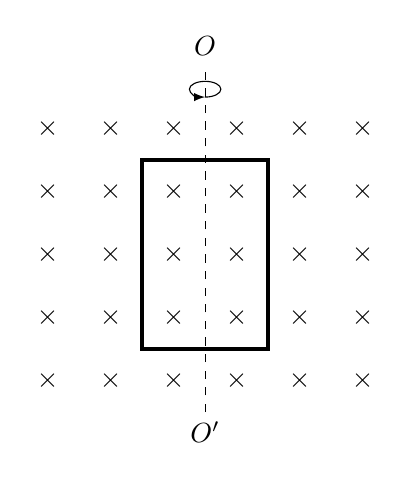
\begin{tikzpicture}[>=latex,scale=0.8]
  % \useasboundingbox(0.9,0)rectangle(5.1,5);
  \foreach \x in {-3,-2,...,2}
  \foreach \y in {-2,...,2}
  {
      \node at (\x,\y){$\times$};
  }
  \draw [dashed](-.5,-2.5)node[below]{$O'$}--(-.5,3)node[above]{$O$};
  \draw[very thick] (-1.5,-1.5) rectangle (.5,1.5);
  \draw[->] (-.5, 2.5) arc [start angle=-90, end angle=270, x radius=.25,y radius=.125];
\end{tikzpicture}
\end{document}
\documentclass{standalone}
\usepackage{tikz}
\usepackage{ctex,siunitx,bm}
\setCJKmainfont{Noto Serif CJK SC}
\usepackage{tkz-euclide,ninecolors}
\usepackage{amsmath}
\usetikzlibrary{patterns, calc}
\usetikzlibrary {decorations.pathmorphing, decorations.pathreplacing, decorations.shapes,}
\begin{document}
\small
\begin{tikzpicture}[>=latex,scale=0.8]
  \draw[densely dashed,azure6](-2.2,-1.4)rectangle(2.2,1.4);
  \foreach \x in {-2.0,-1.2,-0.4,0.4,1.2,2.0}
  {
    \foreach \y in {-1.2,-0.4,0.4,1.2}
    {
      \node at (\x,\y)[azure6]{$\times$};
    }
  }
  \draw(-3.2,-0.2)rectangle(-2.6,0.2);
  \draw[densely dashed](3.2,-0.2)rectangle(2.6,0.2);
  \node at (-2.9,-0.4){1};
  \node at (2.9,-0.4){2};
\end{tikzpicture}
\end{document}
\chapter*{学生实验}
\addcontentsline{toc}{chapter}{学生实验}
\stepcounter{chapter}
\section{验证玻意耳—马略特定律}

在这个实验中,我们用一个带有刻度的注射器近似地验证玻意耳—马略特定律。

实验研究的对象是封闭在注射器里的空气柱。
空气柱的体积可由注射器上的刻度直接读出。
空气柱的压强 $p=p_0\pm \frac{F}{S}$,其中 $p_0$ 为大气压强,$F$ 为活塞对空气柱的压力或拉力,$S$ 为活塞的横截面积。(考虑一下,哪种情况取正号,哪种情况取负号。)

实验时,先用弹簧秤称出活塞和框架的重量。
用刻度尺测出注射器的全部刻度的长度,用这个长度去除它的容积即得活塞的横截面积 $S$。记下气压计(全班共用一个)指示的大气压强 $p_0$。

将活塞插入注射器内一部分后,将注射器的小孔堵住,以封入一定质量的空气。

把注射器固定好。
在框架的两侧加挂钩码,使空气柱的体积减小(\cref{fig:9-1})。改变钩码的个数,再做两次。
记下每次加挂的钩码数和相应的空气柱的体积。
\begin{figure}
  \begin{minipage}[b]{0.48\linewidth}
  \centering
  \includegraphics{9-1.pdf}
  \caption{}\label{fig:9-1}
  \end{minipage}
  \begin{minipage}[b]{0.48\linewidth}
  \centering
  \includegraphics{9-2.pdf}
  \caption{}\label{fig:9-2}
  \end{minipage}
\end{figure}

然后,用弹簧秤钩住活塞框架的上边,慢慢竖直提起活塞,使空气柱的体积增大(\cref{fig:9-2})。
记下三组每提到一定高度时弹簧秤的读数和相应的空气柱的体积。

把记录的数据填入自己设计的表格里。
根据公式 $p=p_0\pm \frac{F}{S}$ 算出各个压强值(要注意活塞和框架的重量对压强的影响)。
求出各个压强 $p$ 跟相应的体积 $V$ 的乘积。
比较这些乘积,能得出什么结论?

\section{验证气体状态方程}
这个实验,我们利用实验一的装置来验证气体状态方程。

跟实验一一样,先用弹簧秤称出活塞和框架的重量;测出注射器的全部刻度的长度,求出活塞的横截面积 $S$;记下这时的大气压强 $p_0$。
在注射器内封入一定质量的空气。

\medskip\noindent
\begin{minipage}{0.7\linewidth}\parindent2em
照\cref{fig:9-3} 那样,固定好注射器和烧杯。
在活塞框架的两侧加挂钩码,用公式 $p=p_0+ \frac{F}{S}$ 计算出空气柱的压强(注意压力 $F$ 中应包括活塞和框架的重量)。
向烧杯里倒入适量的水,使注射器内的空气柱位于水面之下。
经过两分钟左右,用温度计测出水的温度 $t$,可以认为这个温度就是空气柱的温度,把它换算成热力学温度 $T$。
记下这时空气柱的体积 $V$。

改变加挂的钩码数和烧杯中水的温度,再分别做四次上面的实验。
\end{minipage}\hfill
\begin{minipage}{0.25\linewidth}\centering
  \begin{figurehere}
    \includegraphics{9-3.pdf}
    \caption{}\label{fig:9-3}
  \end{figurehere}
\end{minipage}

\medskip
把上面得到的数据填入自己设计的表格里,并算出每次实验得到的 $pV/T$ 的值,看看它们是否相等,从实验可以得出什么结论?

\section{测定冰的熔解热}

单位质量的某种物质熔解成同温度的液体时吸收的热量,叫做这种物质的熔解热。
在这个实验里我们利用量热器用混合法来测定冰的熔解热。

设有 $m_{\text{冰}}\,\unit{g}$ 的冰,温度为 \qty{0}{\celsius},与 $m_{\text{水}}\,\unit{g}$ 温度为 $t_0$ 的水混合,冰全部熔解跟水混合以后的平衡温度为 $t$。
$m_{\text{冰}}\,\unit{g}$ 冰熔解成水并升高到温度 $t$ 吸收的热量,等于 $m_{\text{水}}\,\unit{g}$ 水以及盛水容器从温度 $t_0$ 下降到温度 $t$ 放出的热量,即
\[ m_{\text{冰}}\lambda+m_{\text{冰}}c_{\text{水}}t=(m_{\text{水}}c_{\text{水}}+m_{\text{筒}}c_{\text{筒}})(t_0-t).\]
其中,$\lambda$ 为冰的熔解热,$c_{\text{水}}$ 为水的比热,$c_{\text{筒}}$ 为容器的比热,$m_{\text{筒}}$ 为容器的质量。
这样,把 $c_{\text{水}}$ 和 $c_{\text{筒}}$ 作为已知量,$m_{\text{冰}}$、$m_{\text{水}}$、$m_{\text{筒}}$ 和 $t_0$、$t$ 都可以由实验获得,从而利用上式求出冰的熔解热 $\lambda$。

实验开始时,先用天平称出量热器小筒的质量 $m_{\text{筒}}$(包括搅拌器)。
然后把比室温高 \qtyrange{10}{15}{\celsius} 的温水(\qty{150}{g} 左右)倒入量热器小筒,再称出水和小筒的质量,算出水的质量 $m_{\text{水}}$。
把装着水的量热器小筒放在大筒的木架上,用温度计测出水和量热器小筒的初温 $t_0$。
把准备好的温度为 \qty{0}{\celsius} 的冰块\footnote{实验室里,冰水混合物的温度可以认为是\qty{0}{\celsius}。}(\qty{20}{g} 左右)迅速放入小筒的水中,并盖好量热器盖子。
搅动小筒中的水,同时观察插入量热器里的温度计。
当温度下降到最低时,记录下来的温度 $t$ 就是冰、水混合后的平衡温度。
最后再称量一下量热器小筒和水的质量(其中包括冰的质量),算出冰的质量 $m_{\text{冰}}$。

把由实验得到的数据代入第二段中的公式,求出冰的熔解热。
水的比热 $c_{\text{水}}$,可取为 \qty{4.2e3}{J/(kg.\celsius)},铝制小筒的比热 $c_{\text{筒}}$ 可取为 \qty{8.9e2}{J/(kg.\celsius)},铜制小筒的比热 $c_{\text{筒}}$ 可取为 \qty{3.9e2}{J/(kg.\celsius)}。

实验中要注意读准温度计的示数。
冰块不宜太大,为什么?
在这个实验中,误差的主要来源是什么?

\section{测定空气的相对湿度}
这个实验我们学习测定空气的相对湿度。
实验装置如\cref{fig:9-4} 所示。
圆柱形金属盒的一个底面十分光亮,侧面有开口,开口旁边有一小孔,用来插入温度计。
环形金属片套在金属盒上,它的一面也是十分光亮,井与金属盒的光亮面在同一平面内,金属盒和环形片用胶木垫圈隔开,防止相互间的热传导。
搅拌器插在开口中。

\medskip\noindent
\begin{minipage}{0.6\linewidth}\parindent2em
实验时,先记录下实验室的温度,用柔软的绒布仔细地把金属盒和环形片的光亮面擦得十分干净。
在金属盒里注入约半盒室温的水,再向水里投入适量的碎冰块(注意不要沾污光亮面)。
装上温度计,并使它的刻度向着金属盒的光亮面。
搅动冰块,使水温迅速下降,同时密切注视金属盒和环形片的光亮面,当金属盒的光亮面上刚刚出现细小的露滴时,记录下这一瞬间盒里水的温度。
等水的温度又开始上升,金属盒光亮面上的细小的露滴完全消失时,再记录下这一瞬间的温度,两次温度的平均值就是露点。
\end{minipage}\hfill
\begin{minipage}{0.35\linewidth}\centering
  \begin{figurehere}
    \includegraphics{9-4.pdf}
    \caption{}\label{fig:9-4}
  \end{figurehere}
\end{minipage}

\medskip
从课本里查出温度为测得的露点时水的饱和汽压 $p$,这就是测量时空气中水蒸气的压强,即空气的绝对湿度。
再查出测量时的室温下水的饱和汽压 $P$。
此时的相对湿度就是
\[B=\frac{p}{P}\times 100\%.\]

\section{电场中等势线的描绘}
在这个实验里,我们学习用描迹法画出电场中平面上的等势线。

如\cref{fig:9-5} 所示,在平整的木板上铺一张白纸,白纸上依次铺放复写纸和导电纸,导电纸有导电物质的一面向上。
白纸、复写纸和导电纸一起用图钉固定在木板上。
导电纸上平放着跟它接触良好的两个圆柱形电极,电极 $A$ 与电源的正极相连作为正电荷,电极 $B$ 与电源的负极相连作为负电荷\footnote{我们在\cref{chp:electric_field}学习的是静电场。直接接绘静电场中的等势线是相当困难的,由于静电场和稳恒电流场遵守的规律相似,这里是用在导电纸上形成的稳恒电流场模拟静电场来做实验。}。
两电极之间的距离约为 \qty{10}{cm},电压约为 \qty{6}{V}。
\begin{figure}
  \includegraphics{9-5.pdf}
  \caption{}\label{fig:9-5}
\end{figure}

现在,我们来描绘正、负电荷 $A$、$B$ 在纸面上的等势线。
从灵敏电流表的两个接线柱引出两个探针,用来探测导电纸上的等势点。
先在导电纸平面两电极的连线上,选取间距大致相等的五个点作为基准点,并用探针把它们的位置复印在白纸上。
在某一基准点将一个探针跟导电纸相接触,然后在导电纸平面上两电极连线的一侧,距此基准点约 \qty{1}{cm} 处再选一个点,在此点将另一探针跟导电纸相接触。
一般这时会看到电流表的指针有偏转。
左右移动另一探针的位置,直到找到一点,使电流表的指针没有偏转为止。
电流表的指针没有偏转,说明这个点跟基准点的电势相等。
用探针把这个点的位置复印在白纸上。
照上述方法,在这个基准点的两侧,各探测出五个等势点,每个等势点大约相距 \qty{1}{cm}。
用同样的方法,探测出另外四个基准点的等势点。
最后,取出白纸,根据五组等势点画出五条平滑的曲线,它们就是等势线。
你能不能根据这些等势线在白纸上画出两个异种电荷的电力线:画一画看。

\section{利用电容器放电测电容}
现在,我们通过实验来学习一种测量电容器电容的简单方法。

我们知道,电容器的电容等于电容器所带电量跟两极之间的电势差的比值,即 $C=Q/U$。
因此,如果测量出某一电压下电容器所带的电量,就可以求出电容器的电容。
怎样才能测量出电容器所带的电量呢?
\begin{figure}
  \includegraphics{9-6.pdf}    
  \caption{}\label{fig:9-6}
\end{figure}

测量电路如\cref{fig:9-6} 所示,合上电键 $K'$、$K$,对电容器 $C$ 充电。
当电容器两端电压 $U_c$ 上升到某一稳定电压 $U$ 时,充电完毕。
然后将电键 $K$ 打开,这时容器通过电阻 $R$ 放电,放电电流 $i_c$ 随时间 $t$ 的增加而逐渐减小,放电完毕时 $i_c=0$。
在电容器放电过程中,如果在某一时刻的放电电流为 $i_c$,那么在一小段时间间隔 $\Delta t$ 里,从电容器正极转移到负极上的电量就等于 $i_c\Delta t$,将整个放电过程中每小段时间所转移的电量加起来,就得到电容器所带的电量 $Q$。

按\cref{fig:9-6} 接好线路,电源可用学生电源,电容器 $C$ 可选用 \qty{470}{\micro F} 的电解电容器,微安表可选用 \qty{500}{\micro A} 量程的,$R$ 用 \qty{27}{k\ohm} 的定值电阻,接线时要注意电解电容器的极性不要接反。
接通电源后,先合上电键 $K'$,调节变阻器 $R'$ 使伏特表指示到实验需要的电压值 \qty{12}{V},然后合上电键 $K$,给电容器充电,充电完毕,记下这时伏特表和微安表的读数。
把电键 $K$ 打开,同时开始计时,并且每间隔 \qty{5}{s} 读取一次微安表的电流值,直到电流值减至零为止。

根据记录的数据,在坐标纸上,以时间 $t$ 为横坐标,以电流 $i_c$ 为纵坐标作出 $i_c$--$t$ 图象,然后再根据所画的 $i_c$--$t$ 图象,求出电容器所带电量 $Q$(同学们思考一下,怎样利用 $i_c$--$t$ 图象求出电量 $Q$),最后计算出电容器的电容。

\section{测定金属的电阻率}
这个实验是测定金属的电阻率。

电阻定律告诉我们,用电阻率为 $\rho$ 制成的长 $l\,\unit{m}$、横截面积 $S\,\unit{m^2}$ 的导线的电阻
\[R=\rho\frac{l}{S}.\]

因此,测出一段导线的长度和直径(由直径可以算出横截面积)以及这段导线的电阻,就可以求出制成这段导线的材料的电阻率。

现在有一段长约 \qty{0.5}{m}、直径约 \qty{0.3}{mm},阻值约 \qty{3}{\ohm} 的金属导线,你应当选用哪些实验器材来测定它的电阻率?
考虑一下,这个实验应当怎样进行?
通过实验,你测得制成这段导线的材料的电阻率是多少?

需要注意的是,在给导线通电时,电流不宜太大,想想看,这是为什么?

\section{把电流表改装为伏特表}
我们学习了把电流表改装为安培表和伏特表的原理,在这个实验里,我们练习把电流表改装为伏特表。

改装电流表,需要知道它的三个数据:满度电流 $I_g$,满度电压 $U_g$(电流表的指针偏转到满刻度时加在表头上的电压)和内电阻 $r_g$。
这三个数据中,知道任何两个,就可以根据欧姆定律算出第三个,电流表的 $I_g$ 可以从刻度盘上直接读出,$r_g$ 可用实验方法测出,于是就可以算出 $U_g$。
\begin{figure}
  \includegraphics{9-7.pdf}    
  \caption{}\label{fig:9-7}
\end{figure}

我们利用\cref{fig:9-7} 所示的电路来测定电流表的内电阻 $r_g$。
$R$ 可用 \qty{470}{k\ohm} 的电位器\footnote{电位器是一种可以连续调节电阻值的变阻器,常用作分压器。},$R'$ 是电阻箱,合上电键 $K_1$,调整电位器 $R$,使电流表指针偏转到满刻度(要注意,不应使通过电流表的电流超过它的满度电流值,以免把表烧坏),然后再合上电键 $K_2$,调整电阻箱 $R'$ 的阻值,使电流表指针偏转到正好是满刻度的一半。
当 $R$ 比$R'$ 大很多时,接入 $R$ 后,干路中电流变化不大,因此可以认为 $r_g=R'$。


测出 $r_g$ 后,再计算出电流表的满度电压 $U_g$。
然后算出把它改装为 \qty{2}{V} 的伏特表时,应该串联多大的电阻 $R_1$。
在电阻箱上取好阻值 $R_1$,把电流表跟电阻箱串联起来,就是一个量程是 \qty{2}{V} 的伏特表了。
\begin{figure}
  \begin{minipage}[b]{0.48\linewidth}\centering
    \includegraphics{9-8.pdf}
    \caption{}\label{fig:9-8}
  \end{minipage}
  \begin{minipage}[b]{0.48\linewidth}\centering
    \includegraphics{9-9.pdf}  
    \caption{}\label{fig:9-9}
  \end{minipage}
\end{figure}

最后把改装成的伏特表跟标准伏特表核对一遍。
实验电路如\cref{fig:9-8} 所示,$V$ 是标准伏特表,改变变阻器 $R_2$ 的触点,使 $V$ 的读数分别为 \qty{0.5}{V}、\qty{1}{V}、\qty{1.5}{V}、\qty{2}{V} 时,核对一下改装的伏特表的读数是否正确。
核对时要注意搞清楚改装后电流表上刻度的每一小格表示多大电压。
最后算出改装的伏特表满刻度时的百分误差。
例如改装的伏特表在满刻度 \qty{2}{V} 时,标准伏特表的读数为 \qty{2.1}{V},那么满刻度时的百分误差就是
\[\frac{|2.1-2|}{2.1}=4.8\%.\]

\section{用安培表和伏特表测定电池的电动势和内电阻}
这个实验是用安培表和伏特表测出电流和路端电压,再用闭合电路的欧姆定律来求出电动势和内电阻。
实验电路如\cref{fig:9-9} 所示。

我们知道,只要改变 $R$ 的阻值,测出两组 $I$、$U$ 的数据。代入方程组
\[\begin{split}
    \mathcal{E}&=U_1+I_1r,\\
    \mathcal{E}&=U_2+I_2r.\\
\end{split}\]
就可以求出电动势 $\mathcal{E}$ 和内电阻 $r$,这样做在原理上虽然很简单,但偶然误差却很大。

为了减小偶然误差,我们可以多测出几组 $I$、$U$ 的数据,求出几组 $\mathcal{E}$、$r$ 值,最后分别算出它们的平均值。
此外,物理实验中还经常用作图法,现在我们就来学习作图法。

利用变阻器 $R$ 测出几组 $I$、$U$ 值后,在坐标纸上以 $I$ 为横坐标,$U$ 为纵坐标,画出 $U$--$I$ 关系图象。
根据闭合电路的欧姆定律,$U=\mathcal{E}-Ir$,因此 $U$ 是 $I$ 的一次函数,它们的图象应该是一条直线。
你得出的是不是一条直线?
把这条直线延长,使它跟纵轴相交,这个交点有什么物理意义?
在图象中内电阻是怎样表示出来的?
你怎样利用自己作出的图象来得到电池的电动势和内电阻?

这里还要作一点说明,作图时要适当选取横坐标、纵坐标的比例和坐标的起点,使实验数据大致布满整个图纸,不要集中在一边或一角。
这个实验的 $U$ 值不宜过小,因此纵坐标 $U$ 的起点不要从零开始,而横坐标 $I$ 仍要以零为起点。(为什么?)

\section{练习使用万用电表}
万用电表(常简称为万用表)是一种多用仪表,一般可以用来测量电流、电压、电阻等,并且每一种测量项目有几个量程。
由于万用表具有用途多、量程广、使用方便等优点,因此得到了广泛的应用,这个实验我们来学习万用表的使用。

万用表的型号很多,但使用方法基本相同,下面以 J0411 型万用表为例来说明它的使用方法和注意事项。

\medskip\noindent
\begin{minipage}{0.47\linewidth}\parindent2em
J0411 型万用表的外形如\cref{fig:9-10} 所示。
它的上半部是表头,表盘上有电阻、电流、电压等各种量程的刻度。
有的刻度是均匀的,因此合用一个刻度。
下半部是选择开关,它的四周刻着各种测量项目和量程。
应当注意,电流和电压又分为直流(用符号“$-$”表示)和交流(用符号“$\oldsim$”表示),要区别开,不要弄错。
另外还有欧姆档的调零旋钮和测试笔插孔。

测量前,应先检查表针是否停在左端的“0”位置,否则,要用小螺丝刀轻轻地转动表盘下边中间的调整定位螺丝,使指针指零。
万用表有两根测试笔,将红表笔和黑表笔分别插入正($+$)、负($-$)测试笔插孔。
\end{minipage}\hfill
\begin{minipage}{0.48\linewidth}
  \begin{figurehere}
    \includegraphics{9-10.pdf}
    \caption{}\label{fig:9-10}
  \end{figurehere}
\end{minipage}

\medskip
测量时,应把选择开关旋到相应的项目和量程上。
读数时,要看跟选择开关的档位相应的刻度。

测量电流时,跟电流表一样,应把万用表串联在被测电路里;对于直流电,还必须使电流从红表笔流进万用表,从黑表笔流出来。

测量电压时,跟电压表一样,应把万用表和被测部分并联;对于直流电,必须用红表笔接电势较高的点,用黑表笔接电势较低的点。

测量电阻时,在选择好选择开关的档位后,要先把两根表笔相接触,调整欧姆档的调零旋钮,使指针指在电阻刻度的零位上(注意,电阻刻度的零位在表盘的右端)。
然后再把两表笔分别与待测电阻的两端相接,进行测量。
换用欧姆档的另一量程时,需要重新调整欧姆档的调零旋钮,才能进行测量。
应当注意,测量电阻时待测电阻要跟别的元件和电源断开。(为什么?)

测量时,注意手不要碰到表笔的金属触针,以保证安全和测量的准确;使用后,要把表笔从测试笔插孔拔出,井且不要把选择开关置于欧姆档,以防电池漏电;长期不使用时,应把电池取出。

在了解了你使用的万用表之后,就可以按照老师的要求,来进行电流、电压和电阻的测量了。

\section{用惠斯通电桥测电阻}
这个实验是用滑线式电桥来测电阻。

实验电路如\cref{fig:9-11} 所示,其中 $R_x$ 是待测电阻,$R_0$ 是作已知电阻用的电阻箱,$G$ 是灵敏电流表。
按图接好电路后,先把变阻器 $R$ 调到阻值较大的位置,然后进行实验。
\begin{figure}
  \includegraphics{9-11.pdf}  
  \caption{}\label{fig:9-11}
\end{figure}

根据误差理论,触头 $D$ 在 $AC$ 中点附近电桥平衡时实验误差较小(这个道理在这里就不讲了)。
我们先用万用表测出 $R_x$ 的大约值,在电阻箱上选取跟它接近的某一阻值 $R_0$。
合上电键 $K$,把滑动触头 $D$ 移到电阻线 $AC$ 中点附近某一位置,瞬时按下触头,一般会看到电流表的指针有偏转,稍稍移动触头,再把它瞬时按下,比较电流表指针两次偏转的情况。
根据指针偏转的方向是否相同和偏角是增大还是减小,你应该能判断出应向哪个方向移动触头才能使电桥平衡。
继续移动触头直到电桥平衡,电流表的指针不再偏转为止。
要注意,每次按下触头的时间要尽量短,用力不要过大,更不要在按下触头后又设法移动它。

电桥平衡后,打开电键 $K$,读出或量出 $AD$ 的长度 $l_1$ 和 $DC$ 的长度 $l_2$,根据 $R_0/R_x=l_1/l_2$ 求出 $R_x$,这就初步测出了$R_x$ 的值。

现在来进一步更精确地测定 $R_x$。
先在电阻箱上取跟初步测出的 $R_x$ 相近的阻值,重新使电桥平衡。
然后逐步减少变阻器 $R$ 的阻值,以增大 $AC$ 间的电压,但要注意通过电阻线 $AC$ 的电流不能超过它的允许值。
可以看到,每当 $R$ 的阻值减少后,按下触头$D$ 时电桥又可能不平衡了,每次都要重新调整触头 $D$ 的位置,才能使电桥恢复平衡。
同学们想想看,这是什么道理。
要注意这时每次都只能微调触头 $D$ 的位置,以免烧毁电流表。
当 $R$ 的阻值减小到一定程度时,使电桥平衡,然后读出或量出 $l_1$ 和 $l_2$,利用公式算出 $R_x$。
为什么现在求出的 $R_x$ 比初测的 $R_x$ 精确?

\section{测定铜的电化当量}
在这个实验里,我们根据法拉第电解第一定律 $m=kIt$,测出 $m$、$I$ 和 $t$ 的值,从而确定电化当量 $k$。

\medskip\noindent
\begin{minipage}{0.65\linewidth}\parindent2em
准备三块铜片,两块作为阳极,一块作为阴极,并用细砂纸把铜片擦干净,用天平仔细称量作为阴极的铜片的质量。
把铜片放入盛有硫酸铜溶液的电解槽内。
按照\cref{fig:9-12} 接好电路(注意电源和安培表的正负端不要接错),合上电键 $K$,调节变阻器 $R$ 使安培表的读数为 \qty{2}{A} 左右,并开始计时。
\qtyrange{25}{30}{min} 后,打开电键 $K$,停止电解。
注意要在整个电解过程中,调节变阻器使电流强度保持不变。
电解结束后,取出电极,用酒精灯把阴极板烘干,再用天平仔细称量出这时阴极板的质量。比较两次称量的阴极板的质量,就可以得到电解过程中在阴极板上析出的铜的质量 $m$。
把 $m$、$I$ 和 $t$ 带入法拉第电解第一定律公式,算出铜的电化当量。
\end{minipage}\hfill
\begin{minipage}{0.3\linewidth}\centering
  \begin{figurehere}
    \includegraphics{9-12.pdf}
    \caption{}\label{fig:9-12}
  \end{figurehere}
\end{minipage}

\medskip
你测定的铜的电化当量是多少?
跟课本上给出的数值相差多少?
考虑一下,实验误差的主要原因是什么?
应当怎样改进这个实验?

\section{练习使用示波器}
示波器是一种常用的电子仪器,它的核心部分是一只示波管,利用它能够直接观察电信号随时间而变化的情况,并且可以测量电压和电流。
我们现在初步学习一下示波器的使用方法,在后面的实验里还要多次用到它。

\medskip\noindent
\begin{minipage}{0.4\linewidth}\parindent2em
示波器的型号很多,使用方法基本相同,下面以 J2459 型示波器(\cref{fig:9-13})为例来说明。

我们先来了解示波器面板上各个旋纽和开关的名称和作用。
荧光屏右边最上端的旋钮是辉度调节“\faSun[regular]”,用来调节图象的亮度,顺时针旋转时亮度逐渐增大。
它下面的旋钮是聚焦调节“\faDotCircle[regular]”和辅助聚焦“\faCircle[regular]”,这两个旋钮配合着使用,能使电子射线会聚,在荧光屏上产生一个小的亮斑,得到清晰的图象。
再下面是电源开关和指示灯,用后盖板上的电源插座接通电源后,把开关板向“开”的位置,指示灯亮,经过一两分钟的预热,示波器就可以使用了。
\end{minipage}\hfill
\begin{minipage}{0.55\linewidth}\centering
  \begin{figurehere}
    \includegraphics{9-13.pdf}
    \caption{J2459 型示波器的面板}\label{fig:9-13}
  \end{figurehere}
\end{minipage}

\medskip
荧光屏下边第一行左右两端的旋钮是竖直位移“$\uparrow\downarrow$”和水平位移“$\leftrightarrows$”,分别用来调整图象在竖直方向和水平方向的位置。
它们中间的两个旋钮是“Y 增益”和“X 增益”,分别用来调整图象在竖直方向和水平方向的幅度,顺时针旋转时,幅度连续增大。

中间一行左边的大旋钮是“衰减”,它有 1, 10、100、1000 四档,最左边的“1”档不衰减,其余各档分别使输入电压衰减为原来的 1/10、1/100、1/1000,因此图象在竖直方向的幅度都减小为前一档的十分之一;最右边的正弦符号“\tikz \draw[x=.7ex,y=1ex] (0,0) sin (1,1) cos (2,0) sin (3,-1) cos (4,0)--(0,0);”档不是衰减,而是由示波器内部自行提供竖直方向的交流试验信号电压,可用来观察正弦波形或检查示波器是否正常工作。
右边的大旋钮是“扫描范围”,也有四档,可以改变加在水平方向的扫描电压的频率范围,左边第一档是 \qtyrange{10}{100}{Hz},向右旋转每升高一档,扫描频率都增大 10 倍,最右边的是“外 X”档,使用这一档时,机内没有加扫描电压,水平方向的电压可以从外部输入。
中间的小旋钮是“扫描微调”,用来调整水平方向的扫描频率,顺时针转动时频率连续增加。

底下一行中间的旋钮“Y 输入”、“X 输入”和“地”分别是竖直方向、水平方向和公共接地的输入接线柱。
左边的“DC、AC”是竖直方向输入信号的直流、交流选择开关。
置于“DC”位置时,所加的信号电压是直接输入的;置于“AC”位置时,所加的信号电压是通过一个电容器输入的,它可以让交流信号通过而隔断直流成分。
右边的“同步”也是一个选择开关,置于“$+$”位置时,扫描由被测信号正半周起同步,置于“$-$”位置时,扫描由负半周起同步。

现在,我们来练习使用示波器。
先把辉度调节旋钮反时针转到底,竖直位移和水平位移旋钮旋转到中间位置,衰减旋钮置于最高档,扫描范围旋钮置于“外 X”档,打开电源开关,指示灯亮。
经预热后,顺时针旋转辉度调节旋钮,屏上即出现一个亮斑。
亮斑的亮度要适中,注意不应使亮斑过亮,特别是当亮斑长时间停留在屏上不动时,应把亮度减弱,以免损伤荧光屏,减少示波管的使用寿命。
旋转聚焦调节和辅助聚焦旋钮,观察亮斑的变化,使亮斑最圆最小。
旋转竖直位移旋钮,观察亮斑的上下移动,旋转水平位移旋钮,观察亮斑的左右移动。

把 X 增益旋钮顺时针转到三分之一处,扫描微调旋钮反时针转到底,扫描范围旋钮置于最低档。
可以看到扫描的情形:亮斑从左向右移动,到右端后又很快回到左端,顺时针旋转扫描微调以增大扫描频率,可以看到亮斑迅速移动成为一条亮线。
调整 X 增益,可以看到亮线长度的改变。

现在给竖直方向加一个直流电压。事先把扫描范围旋钮置于“外 X”档,使亮斑位于屏的中心,把“DC、AC”开关置于“DC”位置。
照\cref{fig:9-14} 连接电路,直流电源用一、二节干电池即可。
逐步减小衰减档,观察亮斑的向上偏移,再调整 Y 增益使亮斑偏移一段适当的距离。
调整变阻器改变输入电压,可以看到亮斑的偏移随着改变,电压越高,偏移越大,调换电池的正负极,改变输入电压的方向,可以看到亮斑改为向下偏移。
\begin{figure}
  \includegraphics{9-14.pdf}
  \caption{}\label{fig:9-14}
\end{figure}

亮斑偏移的距离跟输入的电压成正比,因而利用示波器能够测量电压。
J2459 型示波器的竖直位移已经校准。
当衰减旋钮处在“1”的位置,Y 增益旋钮顺时针转到底时,如果输入电压为 \qty{50}{mV},则亮斑恰好偏移 1 格。
这样,我们就可以根据亮斑偏移的格数来算出输入的电压值,测量时要注意把 Y 增益旋钮顺时针转到底;衰减旋钮处在 10、100 或 1000 档时,算出的电压值应乘以相应的倍数。
现在来测一节干电池的电压,你测出的数值是多少?

利用示波器还可以测量电流。
把一个已知阻值的小电阻串联在待测电流的电路里(或利用原电路中的已知电阻),用示波器测量这个电阻两端的电压,利用欧姆定律就可以算出电路中的电流。
这种测量我们就不做了。

实验完了,关机前要注意把辉度调节旋钮反时针方向转到底,使亮度减到最小。
\input{contents/app2-2.tex}
\appendix
\chapter{常用的热学量和电学量的国际单位制单位}

\begin{table}
\begin{tblr}{colspec={ccccX[c]},hline{3}=0.8pt}
\SetCell[c=2]{m,c}{物理量} & & \SetCell[c=2]{m,c}{单位} & &\SetCell[r=2]{m,c} 量纲式\\
名称&符号 &中文符号&英文符号& \\
热力学温度      &  $T$           &  开                & \unit{K}        &  $[\Theta]$   \\
热量            &  $Q$           &  焦                & \unit{J}        &  $[L^2MT^{-2}]$ \\
比热            &  $c$           &  焦/千克$\cdot $开 & \unit{J/(kg.K)} &  $[L^2T^{-2}\Theta^{-1}]$\\  
电流            &  $I$           &  安                & \unit{A}        &  $[I]$ \\
电量            &  $Q$           &  库                & \unit{C}        &  $[TI]$ \\
电场强度        &  $E$           &  伏/米$^2$         & \unit{V/m^2}    &  $[LMT^{-3}I^{-1}]$ \\
电势(差)、电压 &  $U(V)$        &  伏                & \unit{V}        &  $[L^2MT^{-3}I^{-1}]$ \\
电动势          &  $\mathcal{E}$ &  伏                & \unit{V}        &  $[L^2MT^{-3}I^{-1}]$ \\
电容            &  $C$           &  法                & \unit{F}        &  $[L^{-2}M^{-1}T^{4}I^{2}]$ \\
电阻            &  $R$           &  欧                & \unit{\ohm}     &  $[L^{2}MT^{-3}I^{-2}]$ \\
电阻率          &  $\rho$        &  欧$\cdot$米       & \unit{\ohm.m}   &  $[L^{3}MT^{-3}I^{-2}]$ \\
\end{tblr}
\end{table}
\end{document}